% class
\documentclass[en, oneside, onehalfspacing]{risethesis}

% packages and configurations
\usepackage{enumitem}
\usepackage{lineno, hyperref}
\usepackage[numbers]{natbib}
\usepackage{babel}
\usepackage{supertabular}
\usepackage{fancybox}
\usepackage{acronym}
\usepackage{array}
\usepackage{booktabs}
\usepackage{graphicx}
\usepackage{rotating}
\usepackage{tabularx}
\usepackage{color, colortbl}
\usepackage{multirow}
\usepackage{hhline}
\usepackage{setspace}
\usepackage{placeins}
\usepackage{longtable}
\usepackage{amsthm,amsmath}
\usepackage{mathtools}
\usepackage{algorithm}% http://ctan.org/pkg/algorithms
\usepackage{algpseudocode}
\usepackage{listings}
\usepackage{epstopdf}
\usepackage{subfigure}
\usepackage{courier}
\usepackage{amsfonts}
\usepackage{morefloats}
\usepackage{lipsum}
\usepackage{cleveref}
\usepackage{hyperref}

\newtheorem{thm}{Scenario}
\hypersetup{breaklinks=true}
\urlstyle{same}
\Urlmuskip=0mu plus 1mu\relax
\lstset{numbers=left, 
	stepnumber=1, 
	firstnumber=1, 
	numberstyle=\tiny, 
	extendedchars=true, 
	breaklines=true,
	frame=tb,
	basicstyle=\footnotesize, 
	stringstyle=\ttfamily,
	showstringspaces=false
}

\definecolor{lightgray}{gray}{0.8}
\definecolor{Gray}{gray}{0.9}
\renewcommand{\lstlistingname}{Code}
\renewcommand{\lstlistlistingname}{Lista de Listagens}


\DeclarePairedDelimiter\abs{\lvert}{\rvert}%
\DeclarePairedDelimiter\norm{\lVert}{\rVert}%
\DeclareMathOperator*{\argmin}{arg\,min}
\DeclareMathOperator*{\argmax}{arg\,max}
\newcommand*\justify{%
	\fontdimen2\font=0.4em% interword space
	\fontdimen3\font=0.2em% interword stretch
	\fontdimen4\font=0.1em% interword shrink
	\fontdimen7\font=0.1em% extra space
	%\hyphenchar\font=`\-% allowing hyphenation
}

% Algorithmic modifications
\makeatletter
\newcommand{\ALOOP}[1]{\ALC@it\algorithmicloop\ #1%
  \begin{ALC@loop}}
\newcommand{\ENDALOOP}{\end{ALC@loop}\ALC@it\algorithmicendloop}
\renewcommand{\algorithmicrequire}{\textbf{Input:}}
\renewcommand{\algorithmicensure}{\textbf{Output:}}
\newcommand{\algorithmicbreak}{\textbf{break}}
\newcommand{\BREAK}{\STATE \algorithmicbreak}
\makeatother


% 
\address{BRASÍLIA}

\universitypt{Universidade de Brasília}
\universityen{Universidade de Brasília}

\departmentpt{Departamento de Engenharia Elétrica - ENE/FT}
\departmenten{Departamento de Engenharia Elétrica - ENE/FT}

\programpt{Progama de Pós-Graduação em Engenharia Elétrica - PPGEE}
\programen{Progama de Pós-Graduação em Engenharia Elétrica - PPGEE}

\majorfieldpt{Engenharia Elétrica}
\majorfielden{Electrical Engineering}

\title{Discriminative Sensing Based on Signal Processing for Information Security Analysis}
\date{November/2017}

\author{Thiago Pereira de Brito Vieira}
\adviser{João Paulo Carvalho Lustosa da Costa}
% \coadviser{?}

\begin{document}

\frontmatter
\frontpage
\presentationpage

\begin{dedicatory}Ficha Catalográfica\end{dedicatory}

\begin{dedicatory}Signatures\end{dedicatory}

\begin{dedicatory}Dedicatory.\end{dedicatory}

\agradecimentos
First and foremost, I would like to thank God for giving me the life, strength, knowledge and opportunity to undertake this research study and to ..

(...)

Thank You!!

\begin{epigraph}[]{Confucius}
	Wherever you go, go with all your heart.
\end{epigraph}

\resumo
Sistemas distribu�dos t�m sido utilizados na constru��o de modernos servi�os da Internet e infraestrutura de computa��o em n�vem, com o intuito de obter servi�os com alto desempenho, escalabilidade e confiabilidade. Os acordos de n�ves de servi�o adotados pela computa��o na n�vem requerem um reduzido tempo para identificar, diagnosticar e solucionar problemas em sua infraestrutura, de modo a evitar que problemas gerem impactos negativos na qualidade dos servi�os prestados aos seus clientes. Ent�o, a detec��o de causas de erros, diagn�stico e reprodu��o de erros provenientes de sistemas distribu�dos s�o desafios que motivam esfor�os para o desenvolvimento de mecanismos menos intrusivos e mais eficientes, para o monitoramento e depura��o de aplica��es distribu�das em tempo de execu��o. 

A an�lise de tr�fego de rede � uma op��o para a medi��o de sistemas distribu�dos, embora haja limita��es na capacidade de processar grande quantidade de tr�fego de rede em curto tempo, e na escalabilidade para processar tr�fego de rede sob varia��o de demanda de recursos.

O objetivo desta disserta��o � analisar o problema da capacidade de processamento para mensurar sistemas distribu�dos atrav�s da an�lise de  tr�fego de rede, com o intuito de avaliar o desempenho de sistemas distribu�dos de um data center, usando hardware n�o especializado e servi�os de computa��o em n�vem, de uma forma minimamente intrusiva.

N�s propusemos uma nova abordagem baseada em MapReduce para profundamente inspecionar tr�fego de rede de aplica��es distribu�das, com o objetivo de avaliar o desempenho de sistemas distribu�dos em tempo de execu��o, usando hardware n�o especializado. Nesta disserta��o n�s avaliamos a efic�cia do MapReduce para um algoritimo de avalia��o profunda de pacotes, sua capacidade de processamento, o ganho no tempo de conclus�o de tarefas, a escalabilidade na capacidade de processamento, e o comportamento seguido pelas fases do MapReduce, quando aplicado � inspe��o profunda de pacotes, para extrair indicadores de aplica��es distribu�das.

\begin{keywords}
Medi��o de Aplica��es Distribu�das, Depura��o, MapReduce, An�lise de Tr�fego de Rede, An�lise em N�vel de Pacotes, An�lise Profunda de Pacotes
\end{keywords}

\abstract
Distributed systems has been adopted for building modern Internet services and cloud computing infrastructures, in order to obtain services with high performance, scalability, and reliability. Cloud computing SLAs require low time to identify, diagnose and solve problems in a cloud computing production infrastructure, in order to avoid negative impacts into the quality of service provided for its clients. Thus, the detection of error causes, diagnose and reproduction of errors are challenges that motivate efforts to the development of less intrusive mechanisms for monitoring and debugging distributed applications at runtime. 

Network traffic analysis is one option to the distributed systems measurement, although there are limitations on capacity to process large amounts of network traffic in short time, and on scalability to process network traffic where there is variation of resource demand.

The goal of this dissertation is to analyse the processing capacity problem for measuring distributed systems through network traffic analysis, in order to evaluate the performance of distributed systems at a data center, using commodity hardware and cloud computing services, in a minimally intrusive way. 

We propose a new approach based on MapReduce, for deep inspection of distributed application traffic, in order to evaluate the performance of distributed systems at runtime, using commodity hardware. In this dissertation we evaluated the effectiveness of MapReduce for a deep packet inspection algorithm, its processing capacity, completion time speedup, processing capacity scalability, and the behavior followed by MapReduce phases, when applied to deep packet inspection for extracting indicators of distributed applications.

\begin{keywords}
Distributed Application Measurement, Profiling, MapReduce, Network Traffic Analysis, Packet Level Analysis, Deep Packet Inspection
\end{keywords}

\tableofcontents

\makeatletter
\renewcommand{\@thesubfigure}{\thesubfigure:\hskip\subfiglabelskip}
\makeatother
\setcounter{lofdepth}{2}

\listoffigures
\listoftables

\chapter*{List of Acronyms}
\addcontentsline{toc}{chapter}{List of Acronyms}
\begin{acronym}[]
  \acro{DL}{Dictionary Learning}
  \acro{CSF}{Critical Success Factor}
  \acro{PCA}{Principal Component Analysis}  
  \acro{RFE}{Recursive Feature Elimination}
  \acro{SVM}{Support Vector Machines}
  \acro{SRC}{Sparce Representation Classification}
  \acro{IT}{Information Technology}
  \acro{ECDF}{Empirical Cumulative Distribution Function}
  \acro{PC}{Principal Components}
  \acro{SVD}{Singular Value Decomposition}
\end{acronym}
\mainmatter

% Introdução: cenario, motivacao, problema, solucoes atuais, escopo do trabalho, lista de contribuicoes, organizacao do resto do artigo. 
% Chapter Structure
% 	Motivation
% 	Problems Statement
%	Contributions
% 	Dissertation Organization
\chapter{Introduction}
\label{ch:1_introduction}

\begin{quotation}[]{Lao Tzu}
The softest things in the world overcome the hardest things in the world.
\end{quotation}


\section{Motivation}
\label{sc:motivation}

Traditionally, cyber defense methods can be effective against ordinary and conventional types of attacks, yet may fail against innovative malicious techniques \cite{lakhina2005mining}. In order to be able to detect and avoid novel attacks and their variations, it is necessary to develop or improve techniques to achieve efficiency on resource consumption, processing capacity and response time. Moreover, it is crucial to obtain high detection accuracy and capacity to detect variations of malicious patterns. Recently, signal processing schemes have being applied to detect malicious traffic in computer networks \cite{Lu2009,Huang2009,Zonglin2009,david2011blind,da2012improved,tenorio2013greatest, vieira2017model}, showing advances in network traffic analysis.

Information security may consist of both technical and procedural aspects. The former includes equipment and security systems, while the latter corresponds to security rules and recommendations. Intrusion detection and intrusion prevention systems are security systems used, respectively, to detect (passively) and prevent (proactively) threats to computer systems and computer networks. Such systems can work in the following fashions: signature-based, anomaly-based or hybrid \cite{Huang2009,mudzingwa2012study}. Additionally, anomaly detection techniques can be categorized in classification, statistical, information theory and clustering based, according to \cite{bhuyan2014network,ahmed2016survey,osanaiye2016distributed}.

Cloud computing is a new rapidly evolving paradigm in the world of distributed networking and computation. The basic features of the cloud environment is providing elastic, on-demand and secure services for the end-users. While the first two requirements are rather well conceptualized and supported by the majority of the cloud platforms in use, security is a serious concern of the cloud providers and governmental organizations as well as academia and research community \cite{csa2016,higashi2015,gartner2015}. Although for the small and medium-sized enterprises (SME) the cloud environment is often the most cost-effective and easily scalable solution, the security and privacy of the sensitive data in cloud platforms are also not fully conceptualized, leading to obscure and incomplete security paradigms and solutions \cite{galibus2017offline}.

Additional security issues and requirements have to be considered when mobile clients are actively used in corporate cloud environment \cite{yovel2014}. Today organizations and enterprises are adopting the Bring-Your-Own-Device (BYOD) paradigm. The uncontrolled usage of the mobile devices represents a serious risk to the development of secure SME cloud platforms, being the bottleneck of the corporate information security system (ISS). While the enterprise cloud infrastructure based on the web interface can be protected by powerful third-party services, the corporate mobile client is usually light-weighted and generally less protected. 

The protection scheme used on a mobile device should be both computationally secure as well as resource-constrained due to battery power limitations \cite{khan2015cloud}. Therefore, encrypting files and generating keys on a mobile device is not considered a good solution. On the other hand, the protection schemes with good computational qualities lack the security analysis in many cases \cite{khan2014bss}. The common practice is the shadow user activities monitoring \cite{yovel2014}. However, the mobile device usage stays unprotected in all the proposed scenarios while in offline mode. When the mobile client goes offline with the sensitive corporate data on board all powerful cloud-based tools cannot help and the mobile client has to secure itself with its own limited resources. Moreover, due to the resources constraint, there is a crucial difference in strategy of online and offline mode protection.

The field of Mobile Money Transfer (MMT) is a growing market segment and has been motivating investments into security defense and fraud detection. Obtaining access to data sets of mobile transactions for research is a very hard task due to the intrinsic private nature of such transactions. Scientists and researchers must today spend time and effort in obtaining access to relevant data sets before they can research on such data set. However, PaySim \cite{lopez2016paysim} is a financial simulator that simulates mobile money transactions based on an original dataset and provides a synthetic dataset as an approach to such a problem.

Recent developments in science and technology have enabled the growth and availability of raw data to occur at an explosive rate. This has created an immense opportunity for knowledge discovery and data engineering research to play an essential role in a wide range of applications from daily civilian life to national security. Despite the actual high availability of information, the relevant information of some observations is generally of under much reduced dimensionality compared to available data sets. The extraction of relevant information by identifying the generating causes within classes of signals is useful for classification problems and for security analysis. 

The high availability of raw data increases the challenges related to big data analytics and to imbalanced data, which corresponds to data sets exhibiting significant imbalances of classes or rare events of some classes. The fundamental issue with the imbalanced learning problem is the ability of imbalanced data to significantly compromise the performance of most standard learning algorithms. Data analysis of imbalanced data is challenging for classification and prediction problems related to anomaly detection, novelty detection, fraud detection and attack detection. 

Considering that imbalanced data can be composed by rare or unknown events, adaptive techniques can be useful in order to improve models and be able to react to changes or unknown patterns and maintain acceptable performance for classification algorithms. Adaptive techniques are also important for online data analysis or streaming processing, where an incremental processing approach can be applied to deal with high throughput data analysis.

Compressed Sensing (CS) aims to obtain the most relevant information of a dataset, what makes it useful for compression, signal reconstruction, image processing and classification, such as in sparse representation classification (SRC) problems. Dictionary learning is related to CS but seeks to obtain compact and meaningful signal representations, known as dictionary, from learning algorithms or models. DL is a signal processing technique for sparse representation of signals as basis vectors, learning the representations from training data, as dictionaries. DL is based on the principle that some observations can be described by a sparse subset of atoms taken from a redundant dictionary, which represents the causes of some observations of the world. The sparse representation in terms of such dictionaries has attracted increased interest for compressive sensing and for solving problems such as denoising, compression, image processing, data decomposition, feature extraction and classification \cite{tosic2011dictionary, zhang2010discriminative, zhu2016coupled,ravishankar2011mr}. 

Dictionaries are either available analytically, or can be learned from a suitable training set. DL can be formulated as an adaptive algorithm that learns from training data that is updated to represent changes or to adapt to new patterns. Iterative dictionary learning has been used as a blind technique for feature extraction, improving classification without require feature selection or principal component analysis

In some applications, the data and its dictionary are multidimensional, e.g., when estimating jointly behavior of users in social networks. Computing tensor decompositions of multi-way datasets is particularly useful to extract hidden patterns and structure in multidimensional data analytics problems \cite{kolda2009tensor}. Tensor-based algorithms for dictionary learning can improve the performance for cases of multidimensional and separable data, regarding the dictionary identification rating, the required number of training samples and iterations for the optimization problem \cite{roemer2014tensor}. Existing dictionary learning schemes can be applied to multidimensional analysis and obtain valuable results. Additionally, the performance of tensor-based algorithms for recovering of a known separable dictionary outperform existing schemes when dealing with growing multidimensional datasets.


\section{Problem Statement}
\label{sc:problems}

Considering the above described landscape, this thesis outlines the development and evaluation of approaches based on signal processing for information security analysis, through methods to make the data discriminative and able to identify structures, hidden patterns and the most relevant information for network attack detection, mobile malicious behavior analysis and fraud detection in mobile money transactions.

In the context of anomaly-based schemes, this thesis proposes a statistical approach based on signal processing techniques for detection of malicious traffic in computer networks. Inspired by \cite{david2011blind,da2012improved}, this thesis models the network traffic using a signal processing formulation as a composition of three components: legitimate traffic, malicious traffic and noise, taking into account the incoming and outgoing traffic in certain types of network ports (TCP or UDP). The proposed technique is based on eigenvalue analysis, model order selection (MOS) and similarity analysis. In contrast to \cite{david2011blind,da2012improved,tenorio2013greatest}, MOS and eigenvalue analysis are applied to detect time frames under attack. In addition, we also evaluate the accuracy and performance of the proposed framework applied to a experimental scenario and to the DARPA 1998 dataset \citep{osanaiye2016distributed}, which is a well known network traffic dataset. Furthermore, this proposed approach has its accuracy evaluation based on eigen similarity analysis for extracting detailed information about accurate time and network ports under attack.

This thesis also proposes an architecture and approach based on user behavior analysis of mobile apps through Model Order Selection (MOS) \cite{tenorio2013greatest}, in order to detect possible threats, and to reduce the risks and the harm of the most common security threats to offline corporate mobile apps, which are the expired user misusing password and the intruder attack. Additionally, the behavioral analysis can indicate well known malicious behaviors, their variations, as well as novel attacks, which present low or high variance in comparison to legitimate user behaviors. The main target of this proposed solution is to provide a maximum defense at the minimal resource cost.

Considering that big data problems require techniques to deal with multidimensional data in order to make sense of structure and relationship of many dimensions, and also considering that a key challenge to use sparse coding and dictionary learning for classification is how to find proper dictionaries and coefficients that highlight discriminative structure and relationships of one dataset, we also propose a tensor-based dictionary learning method for fraud detection from imbalanced data, in order to apply the tensor decomposition for dictionary learning methods to evidentiate the discriminative sensing of a fraud detection dataset. Specifically, we propose to apply a sparse representation based classification (SRC) method through learning a tensor-based dictionary and evaluate the reconstruction error for fraud classification of mobile money transactions. We propose to use tensor-based dictionary learning for learning fraudulent and legitimate data separately, and apply the learned dictionaries to reconstruct a test signal and classify it as fraud or legitimate, according to the minimum reconstruction error measured by some metrics.


\section{Contributions}
\label{sc:contributions}

We analyze problems related to detection of information security issues and propose new approaches to improve malicious behavior detection through signal processing techniques. The results of the work presented in this thesis provide the following contributions:

\begin{enumerate}
	\item We propose an approach based on eigen similarity analysis for extracting detailed information about accurate time and network ports under network attack, and evaluated the accuracy and performance of the proposed framework applied to an experimental scenario and to the DARPA 1998 dataset;
	\item We discuss the computational complexity of the proposed framework and evaluate the required processing time for tested scenarios;
	\item We propose an architecture and techniques for offline behavioral analysis of a corporate mobile client security architecture;
	\item We discuss the processing time of the proposed framework for mobile devices;
	\item We propose a tensor-based dictionary learning approach for fraud detection in mobile payment transactions;
\end{enumerate}

\section{Thesis Organization}
\label{sc:organization}

This thesis is organized as follows. In Chapter \ref{ch:2_mos_eig_sim}, we propose a statistical approach based on signal processing techniques for detection of malicious traffic in computer networks, based on eigenvalue analysis, model order selection (MOS) and similarity analysis. Chapter \ref{ch:3_mobile} presents an evaluation of an approach and architecture based on user behavior analysis through Model Order Selection (MOS) \cite{tenorio2013greatest}, in order to detect possible threats in a mobile application. Chapter \ref{ch:4_tensor_dl} proposes a tensor-based dictionary learning approach for fraud detection from mobile payment transactions. Chapter \ref{ch:5_conclusionfuturework} draws the conclusions and the suggestions for future work. Furthermore, the Appendix \ref{apx:a_mos} presents mathematical concepts of examples of state-of-the-art MOS schemes and the Appendix \ref{apx:b_csf_fs} presents a critical factors analysis based on Principal Component Analysis (PCA) for visual discriminant analysis, and presents an approach based on Recursive Feature Elimination (RFE) combined with Support Vector Machine (SVM) \cite{hearst1998support}, applied to the survey that evaluates the IT governance of Brazilian public organizations, in order to identify the Critical Success Factors (CSF) for IT governance of the public sector according to TCU.
\chapter{Eigensim - Model Order Selection and Eigen Similarity based Framework for Detection and Identification of Network Attacks}
\label{ch:2_mos_eig_sim}

\begin{quotation}[]{Lao Tzu}
All difficult things have their origin in that which is easy, and great things in that which is small. 
\end{quotation}

Traditionally, cyber defense methods can be effective against ordinary and conventional types of attacks, yet may fail against innovative malicious techniques \cite{lakhina2005mining}. In order to be able to detect and avoid novel attacks and their variations, it is necessary to develop or improve techniques to achieve efficiency on resource consumption, processing capacity and response time. Moreover, it is crucial to obtain high detection accuracy and capacity to detect variations of malicious patterns. Recently, signal processing schemes have being applied to the detection of malicious traffic in computer networks \cite{Lu2009,Huang2009,Zonglin2009,david2011blind,da2012improved,tenorio2013greatest}, showing advances in network traffic analysis.

Information security may consist of both technical and procedural aspects. The former includes equipment and security systems, while the latter corresponds to security rules and recommendations. Intrusion detection and intrusion prevention systems are security systems used, respectively, to detect (passively) and prevent (proactively) threats to computer systems and computer networks. Such systems can work in the following fashions: signature-based, anomaly-based or hybrid \cite{Huang2009,mudzingwa2012study}. Additionally, anomaly detection techniques can be categorized in classification, statistical, information theory and clustering based, according to \cite{bhuyan2014network,ahmed2016survey,osanaiye2016distributed}.

This chapter proposes the Eigensim, which is an approach based on signal processing concepts applied to detection of malicious traffic in computer networks. Inspired by \cite{david2011blind,da2012improved}, the Eigensim models the network traffic using a signal processing formulation as a composition of three components: signal, artifact and noise, taking into account the incoming and outgoing traffic in certain types of network ports (TCP or UDP). The Eigensim is based on eigenvalue analysis, model order selection (MOS) and similarity analysis between eigenvectors. In contrast to \cite{david2011blind,da2012improved,tenorio2013greatest}, MOS and eigenvalue analysis are applied to detect time frames under attack. In addition, we evaluate the accuracy and performance of the proposed framework applied to a experimental scenario and to the DARPA 1998 data set \citep{osanaiye2016distributed}, which is a well known network traffic data set. 

The performed experiments show that synflood, fraggle and port scan attacks can be detected accurately and with great detail in an automatic and blind fashion, i.e. in an unsupervised approach, applying signal processing concepts for traffic modeling and through approaches based on MOS and eigen similarity analysis. The main contributions of the proposed framework are the capability to blindly detect time frames under network attack via MOS and eigen analysis, and the detailed identification of the network attack via eigen similarity analysis.

This chapter is organized as follows. In Section \ref{sec:2_relatedworks}, related works are discussed. Section \ref{sec:2_datamodel} presents the data model and the evaluated data sets. Section \ref{sec:2_prop_getv} describes the proposed framework for blind and automatic detection of flood and probe attacks. Section \ref{sec:2_experimentalresults} discusses the experimental validation and presents the results, and Section \ref{sec:2_Complexity} discusses the computational complexity of the proposed framework and evaluates the required processing time for tested scenarios. Section \ref{sec:2_conclusionandfutureworks} draws the conclusions and the suggestions for future work. The Appendix \ref{apx:a_mos} presents mathematical concepts of examples of state-of-the-art MOS schemes.


\section{Related Works}
\label{sec:2_relatedworks}

Several methods have been proposed for the identification and characterization of malicious activity in computer networks. Classical methods typically employ data mining \cite{he2008applying,ghourabi2010data,osanaiye2016distributed} and regular file analysis \cite{raynal2004honeypot} to detect patterns that indicate the presence of specific attacks in network traffic.

Data mining is often used to describe the process of extracting useful information from large databases. Multiple methods of data mining are used in \cite{he2008applying,osanaiye2016distributed} to analyze data flow in a network with the aim of identifying characteristics of malicious traffic in large scale environments. Researchers have applied data mining techniques in log analysis \cite{ghourabi2010data} to improve intrusion detection performance. However, data mining techniques used so far in network analysis require prior collection of large data sets, which is a limitation of several schemes for online analysis \cite{Huang2009}.

Regular file analysis \cite{raynal2004honeypot} consists of traffic analysis for detecting known patterns that indicate the presence of attacks, applying statistical analysis to the study of collected traffic. An essential feature of this method is that it depends on prior knowledge of the details of the attacks to be identified, and also depends on previous log collection for traffic analysis and false positives reduction.

Principal Component Analysis (PCA) is a statistical technique commonly used for dimensionality reduction. It uses an orthogonal transformation to convert a set of correlated variables into a new subspace of linearly uncorrelated variables, by means of eigenvalue value decomposition, where the first principal components have the largest variance. PCA has been used in attack detection \cite{almotairi2009technique}, considering that this technique is very sensitive to outliers and adopted for classification problems. However, PCA requires human intervention in order to identify abnormalities based on the eigenvalues profiles, if used without complementary techniques.

Callegari \emph{et al} \cite{Zonglin2009} proposed a PCA-based method for identifying the traffic flows responsible for an anomaly detected at the aggregate level and evaluated their proposal through a data set with synthetic anomalies added in the data. However, Callegari \emph{et al} focus on flood attack detection, not addressing probe attack detection, and their approach relies on visual analysis. 

Lee \emph{et al.} \cite{Lee2013} presented the OverSampling PCA (osPCA), which allows one to determine the anomaly of the target instance according to the variation of the resulting dominant eigenvector obtained by similarity analysis and over sampling. In contrast to Lee \emph{et al.}, the Eigensim applies MOS for detection of time frames under attack and similarity analysis to extract details for detection of time and ports under attack. Additionally, Lee \emph{et al.} only evaluate their proposed scheme for covariance analysis, while we adopt an analysis based on sample covariance of zero mean variables and sample covariance of zero mean and unitary standard deviation variables, for flood and probe attacks, respectively. 

Signal processing techniques have been successfully applied to network anomaly detection \cite{Lu2009}. Lu and Ghorbani \cite{Lu2009} proposed a network anomaly detection model based on network flow, wavelet approximation, and system identification theory. However, their work requires a training method to produce a prediction model for normal daily traffic and presents limitations on identification of behaviors without significant outliers, such as port scan attacks. Zonglin \emph{et al} \cite{Zonglin2009} proposed a signal processing method to detect traffic anomaly with correlation analysis, where the correlation between traffic signals and the predicted traffic signals are used to reveal anomalies. Zonglin \emph{et al.} \cite{Zonglin2009} evaluated the correlation analysis for anomaly detection, but the work is not applied to probe and flood attack detection, simultaneously.

The data collected from honeypot systems, such as captured traffic and operating system logs, can be analyzed to obtain information about attack techniques, general trends of threats and exploits. Blind automatic detection of malicious traffic techniques have been developed for honeypots in \cite{david2011blind,da2012improved}. However, traffic on honeypot is simpler than real network traffic, because there are no running legitimate applications, i.e. background traffic, due to the fact that honeypots emulate behavior of a host within a network to deceive and lure attackers \cite{zakaria2012review}. Since honeypots do not generate legitimate traffic, the amount of data captured in honeypots is significantly lower in comparison to a Network Intrusion Detection System (NIDS), which captures and analyzes the largest possible amount of network traffic \cite{david2011blind}. MOS for blind identification of malicious activities in honeypots was proposed by us in \cite{david2011blind}, which evaluated criteria for selecting the model order, through simulations and comparing the order of the resulting model with the true model order.

The proposed framework does not require either a significant amount of logs to detect attacks, nor prior data collection, in order to make comparisons and evaluate the existence of malicious traffic. The proposed solution is automatic and blind for detection of time frames under probe and flood attacks through MOS and eigen analysis. Moreover, we apply eigen similarity analysis to identify details of time and ports under network attacks.

Several approaches for network attack detection uses the KDD 99 \cite{ji2016multi,ahmed2016survey,osanaiye2016distributed,bhuyan2014network} data sets for accuracy and performance evaluation, due to their availability and labeled attacks. Even though the KDD 99 data set are criticized by for the generation procedure and the risk of over-estimations of anomaly detection due to data redundancy, it still represents one of the few publicly available labeled data sets adopted by researchers \cite{osanaiye2016distributed,bhuyan2014network}. 

NSL-KDD \cite{tavallaee2009detailed} data set is the refined version of the KDD 99 data set that redundant data records are removed, in order to avoid biased classifications. Additionally, some approaches uses simulated \cite{callegari2011novel} scenarios or non-public data sets their evaluations. Since the proposed approach relies on a packet level analysis and the KDD 99 and NSL-KDD data sets adopt a traffic aggregation by connections, we consider the use of a experimental scenario on a real network and the DARPA 1998 data set, which is the source for the creation of the KDD 99 and NSL-KDD datas ets. Note that the proposed approach is not based on learning or classification techniques, which are more susceptible to biased results caused by the issues in the DARPA/KDD data sets.


\section{Data Model}
\label{sec:2_datamodel}

In this work, scalars are denoted by italic letters ($a, b, A, B, \alpha, \beta$), vectors by lowercase bold letters (\textbf{a, b}), matrices by uppercase bold letters (\textbf{A, B}), and $a_i,_j$ denotes the (\emph{i, j}) elements of the matrix \textbf{A}. The superscripts \textsuperscript{T} and \textsuperscript{-1} are used for matrix transposition and matrix inversion, respectively. We define the operator $\rm diag(\cdot)$ that returns the vector of the main diagonal of a given matrix, the operator $\rightarrow$, which denotes the deletion of a given element from a set and the operator $\#$, that returns the rank of a matrix, and the operator $\sim$ that sorts the elements of a vector in ascending order.

This section also presents details of the experimental scenario and the selected cases of the DARPA data set, along with a description of the data set model as a signal superposition of signal, artifact and noise, that refer to legitimate, control and malicious traffic. Subsection \ref{sec:2_DataCollection} describes the environment and scenario adopted in order to reproduce flood and probe attacks. Subsection \ref{sec:2_ModelingData} presents how network traffic can be modeled as signal superposition. Subsection \ref{sec:2_SynfloodFraggleandPortscan} details the traffic of synflood, fraggle and port scan attacks, and Subsection \ref{sec:2_Darpadata set} discusses the use of the DARPA data set for evaluation of the proposed approach.

\subsection{Analyzed Scenario and Data Collection}
\label{sec:2_DataCollection}

The environment of the analyzed scenario is composed by two computers and one router, with access to the Internet and to an internal network. In this scenario we performed the simulation of legitimate traffic, control, flood and port scan attacks. During the traffic generation, one computer assumes the role of the attacker, while the other is the victim, according to scenario represented by Figure \ref{fig:2.01}. The victim generate legitimate traffic by means of ordinary use of Internet resources, and control traffic is constantly generated for purposes of network administration and monitoring.

%TODO - recreate the figure and change the concepts
\begin{figure}[h!]
     \centering 
     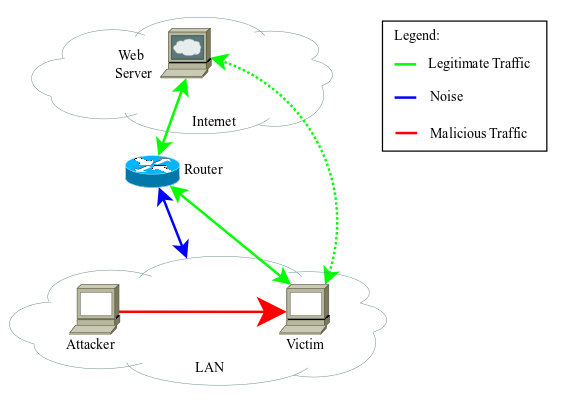
\includegraphics[width=11cm]{figures/fig09.png}
     \caption{Scenario to reproduce legitimate traffic, noise, flood and port scan.}
     \label{fig:2.01}
\end{figure}

Note that the set of network traffic is modeled as legitimate, controls and malicious traffic, which refer to signal, artifact and noise, respectively. In many organizations the web based traffic is predominant, since most of corporate services are  web pages, customized web-based systems and cloud services. It is possible to characterize the traffic of a DHCP service as an example of artifact associated with the transport layer, as well as it would be possible to classify heart beat traffic and other seasonal and controlled traffic as artifact. For malicious traffic, three types of networks attacks are evaluated: synflood, fraggle and port scan. Here we refer to port scan as an attack, according to \cite{ahmed2016survey,moustafa2019holistic}, however it is one approach usually adopted for acquire information in order to perform an attack. These attacks are reproduced using well-known security tools, such as Nmap\footnote{http://nmap.org} for port scan, Metasploit\footnote{http://www.metasploit.com} for synflood and Hping\footnote{http://hping.org} to lead the fraggle attack.

A network traffic log is commonly formed by timestamp, protocol, source IP address, source port, destination IP address, destination port and additional information, according to the type of the used transport protocol. The following TCP traffic log is presented in order to exemplify the collected data:
\newline
\newline
\texttt{\justify21:00:34.099289 IP 192.168.1.102.34712 > 200.221.2.45.80: Flags [S], seq 2424058224, win 14600, options [mss 1460, sackOK,TS val 244136 ecr 0,nop,wscale 7], length 0}
\newline

and the following to exemplify UDP traffic log: 
\newline
\newline
\texttt{\justify21:24:42.484858 IP 192.168.1.102.68 > 192.168.1.1.67: BOOTP/DHCP, Request from 00:26:9e:b7:82:be, length 300}
\newline 

In the proposed framework, the goal is to detect the anomalies only taking into account the traffic profile, i.e. specific information such as origin or destination IP, behavioral pattern or content of the attack are not considered. Therefore, IP spoofing or data encryption would not cause impact to the proposed approach and evaluation, since our proposal only relies on the timestamp (for sequencing) and port number.

\subsection{Modeling Data}
\label{sec:2_ModelingData}

By modeling the data set as a signal superposition, the network traffic (\textbf{X}) can be characterized as a mixture of three components: legitimate traffic (\textbf{U}), artifact (\textbf{A}) and malicious traffic (\textbf{N}), according to the following expression:

\begin{equation}\label{eq:2.01}
	\boldsymbol{X}^{(q)} = \boldsymbol{U}^{(q)} + \boldsymbol{A}^{(q)} + \boldsymbol{N}^{(q)},
\end{equation}
where $q$ represents the $q$-th time frame, which is a time aggregation of network traffic. The matrix $\boldsymbol{X}^{(q)} \in \mathbb{R}^{M \times N}$ consists of \emph{M} rows and \emph{N} columns, where each row represents a communication port, and each column represents time bins of a defined size, such as one minute. Each element $x_{m,n}^{(q)}$ stands for the number packets that appears at $n$-th minute for the port $m$, during the $q$-th time frame.

The legitimate traffic $\boldsymbol{U}^{(q)}$ is characterized by the traffic from user's ordinary operations, such as when performing access to web pages, as well when there is the traffic required to domain name resolution. Figure \ref{fig:2.03} depicts an example of the legitimate traffic simulated during the experiments.

% TODO - Replace
\begin{figure}[h!]
     \centering 
     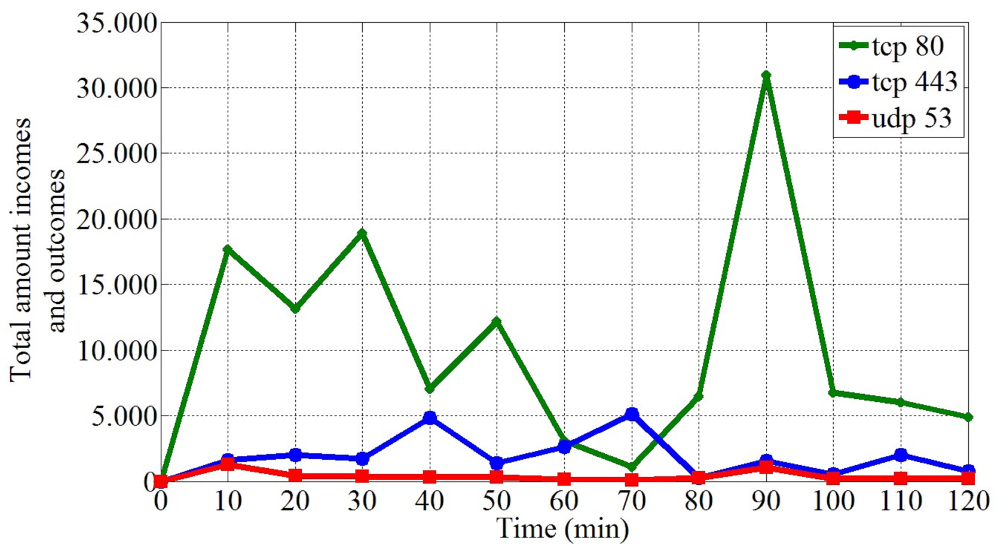
\includegraphics[width=11cm]{figures/fig03.png}
     \caption{Traffic from user's operations, that can be characterized by web access, traffic of well-known applications or network protocols.}
     \label{fig:2.03}
\end{figure}

The traffic that is not associated with user's operations and with malicious traffic is modeled as artifact $\boldsymbol{A}^{(q)}$. The acquisition of logical IP network address (DHCP) is an example of artifact, where independently of any user operation, the machine receives an IP address, since it is configured to automatically perform a DHCP address request. Figure \ref{fig:2.04} depicts an example of artifact in a network traffic, by means of traffic to ports 67 and 68. The traffic coming from a malicious activity, i.e. port scanning, synflood or fraggle attacks, is represented by the matrix $\boldsymbol{N}^{(q)}$.

% TODO - Replace
\begin{figure}[h!]
     \centering 
     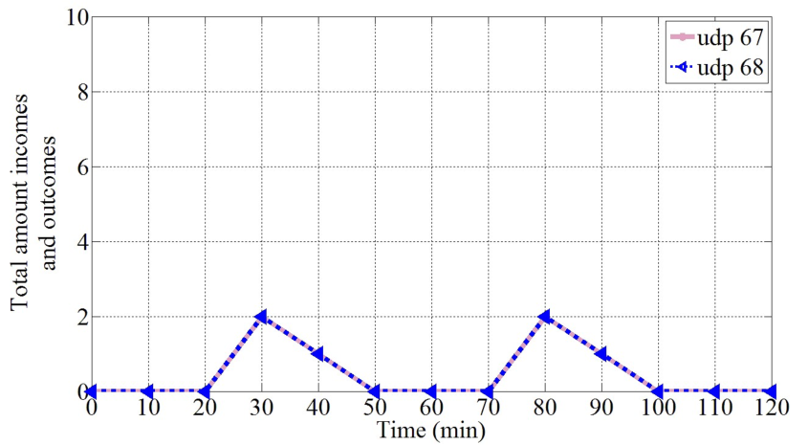
\includegraphics[width=11cm]{figures/fig04.png}
     \caption{Network traffic of user independent operations for network management.}
     \label{fig:2.04}
\end{figure}

We define that if the $\#\boldsymbol{X}^{(q)} ≠ 0$, then there is malicious traffic in the evaluated time frame $q$, on the other hand, if the $\#\boldsymbol{X}^{(q)} = 0$, then there is no malicious traffic. We show how to detect the $\#\boldsymbol{X}^{(q)}$, given only the matrix $\boldsymbol{X}^{(q)}$, in order to identify malicious traffic.

\subsection{Synflood, Fraggle and Port scan}
\label{sec:2_SynfloodFraggleandPortscan}

The network attacks evaluated by this work are: synflood, fraggle and port scan. The first two attacks can be qualified as flood or denial of service (DoS) attacks, while the last one can be qualified as probe or port scanning attack. 

A DoS is an attempt by an attacker to prevent legitimate access to websites by overwhelming the amount of available bandwidth or resources of the computer system. DoS is implemented by either forcing targets to be unavailable through the exploiting of system vulnerabilities, or consuming resources through large amount of network traffic, characterizing flood attacks.

Probe attacks scan computer and network systems to collect information about the host, such as open ports, topology, running software or version of technologies, in order to find vulnerabilities.

With respect to the synflood attacks, the attacker sends a large quantity and concurrent successive SYN requests to a target, in order to consume resources and cause a DoS. Figure \ref{fig:2.05} depicts an example of a synflood attack carried out in a real computer network. In an interval of ten minutes, more than 210,000 packets are sent as a synflood attack. This network traffic behavior can be considered an abnormal behavior of network traffic, especially since it is concentrated in a short period of time and presents similar outstanding traffic during the time under attack.

% TODO - Replace
\begin{figure}[h!]
     \centering 
     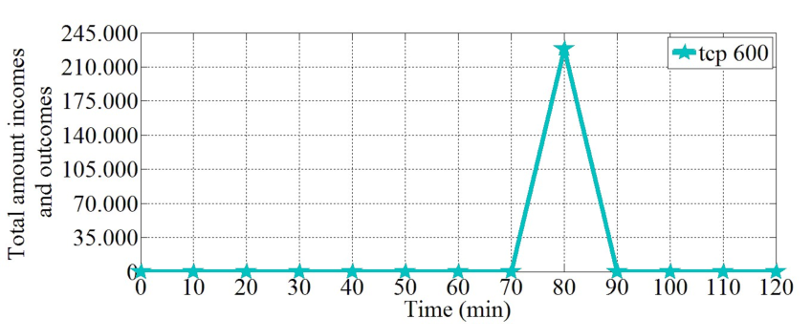
\includegraphics[width=11cm]{figures/fig05.png}
     \caption{A large quantity of SYN requests to a target, in order to cause a DoS.}
     \label{fig:2.05}
\end{figure}

Regarding the fraggle attack, large packets with UDP echo segments are sent to the broadcast address of a network. Every packet is modified to have the source address of the victim, in order to implement the source address spoofing technique. Therefore, each host receives a huge amount of requests UDP echo and all of them replies to the IP address of the victim, causing a packet flooding aiming a DoS. Figure \ref{fig:2.06} depicts an example of the fraggle attack in a real computer network. 

The fraggle attack can affect the entire network, since all hosts receive several requests UDP echo and respond with the ICMP protocol, therefore each host acts as an amplifier of the attack. This part of the fraggle attack is not taken into account in this work, because the victim receives ICMP (network layer) packets originated from the hosts that are attacked with flooding packet UDP echo.

% TODO - Replace
\begin{figure}[h!]
     \centering 
     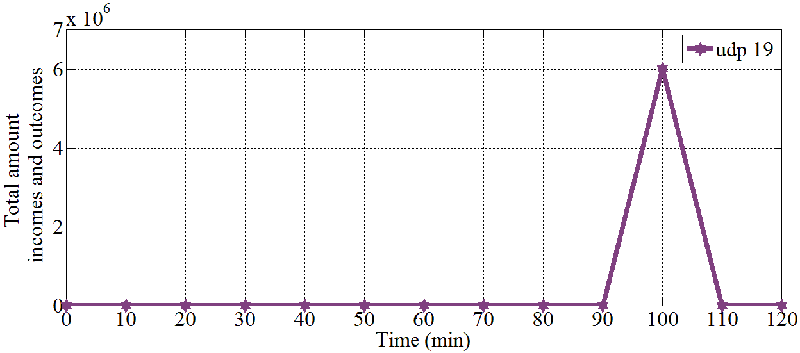
\includegraphics[width=11cm]{figures/fig06.png}
     \caption{Large amount of “UDP echo” requests and replies, causing packet flooding.}
     \label{fig:2.06}
\end{figure}

The Figure \ref{fig:2.06} shows that more than 6,000,000 malicious packets can be counted in an interval of ten minutes, which can be considered an abnormal network traffic, especially due to the concentrated traffic in a short period of time and due to the similarity of the outstanding traffic.

Port scan is the attempt to establish a connection to TCP and UDP ports to identify what services are running or are in the listening state. There are several available port scanning techniques, including: TCP SYN scan, TCP ACK scan and UDP scan. This work evaluates the use of TCP SYN scan and UDP scan. 

In TCP SYN scan, a SYN packet is sent to the destination and two types of responses may occur: SYN/ACK or RST/ACK. In the first case, the destination port is in the listening state, in the second case, the destination port is not listening. At the end of each port scanning, a RST/ACK packet is sent by the system that is performing the port scan. Therefore, a full connection or a complete three-way handshake is never established, which makes the detection of the attack sender more difficult, and requires approaches able to identify probe attacks without connection establishment.

The UDP scan technique sends UDP packets to the destination port, and if it responds with a \emph{ICMP port unreachable} message, then it indicates that the scanned port is closed. On the other hand, if a message is not received, then the port is considered as open.

\begin{figure}[h!]
     \centering 
     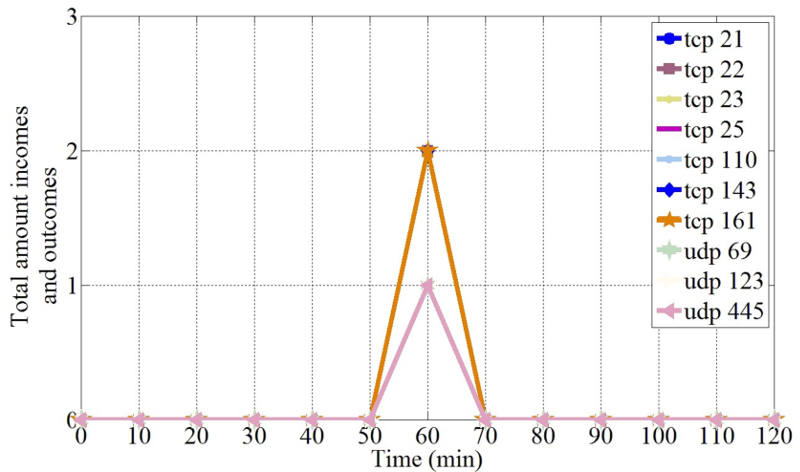
\includegraphics[width=11cm]{figures/fig07.png}
     \caption{Connection attempts in order to identify active ports.}
     \label{fig:2.07}
\end{figure}

Figure \ref{fig:2.07} depicts an example of the port scan attack in a real computer network. Note that the traffic is composed of two packets for each TCP port and one UDP packet to each port. The incoming and outgoing packets analysis, for each port, shows the high correlation and similarity of TCP and UDP traffic during the simulated port scan attack.

\subsection{The DARPA Data set}
\label{sec:2_Darpadata set}

The DARPA 1998 data set\footnote{https://www.ll.mit.edu/ideval/data/} includes 7 weeks of sniffed traffic saved into raw TCPDUMP packet data, from inside and outside origins, with labeled attacks. The attacks in this data set can be grouped into: denial-of-service (DoS); remote to local (R2L), which is characterized by unauthorized access from a remote machine; user to root (U2R), which is characterized by unauthorized access to local super-user privileges; and probe attack. Since the proposed approach focus on flood and probe attack, the analysis concentrates on the attacks of the DARPA 1998 data set that present behaviors similar to flood or probe attack. 

We observe that the most cases of DoS of DARPA 98 focus on exploit system vulnerabilities instead of on flooding attack. One example is the occurrence of a neptune attack which sends 20 SYN packets, what is a behavior that differs of the expected flooding attack behavior. Therefore, there were selected the cases that simulates several network traffic or numerous connection requests, also known as flooding attack \cite{ahmed2016survey,osanaiye2016distributed}, and the cases that scan ports sending just a few packets. From the simulated probe attacks, we select the cases that rely on TCP or UDP connections.

The data modeling follows the method described by the Subsection \ref{sec:2_ModelingData}, with time frames of 20 minutes, packet aggregation counting by minute and considering the traffic to the following ports: 20, 21, 22, 23, 25, 79, 80, 88, 107, 109, 110, 113, 115, 143, 161, 389, 443.


\section{Proposed Framework for Detection and Identification of Network Attacks}
\label{sec:2_prop_getv}

This section describes the proposed technique to detect synflood, fraggle and port scan, according to the overview depicted in Figure \ref{fig:2.08}, which represents the proposed framework for detection and identification of network attacks. In Subsection \ref{sec:2_prop_LargestEigenvaluebyTimeFrames} we present the steps for extraction of the largest eigenvalue for each $q$-th time frame. Next, in Subsection \ref{sec:2_prop_MOSSchemes}, we show how to apply the eigenvalues on the MOS scheme in order to detect the attack. In Subsection \ref{sec:2_prop_EigenvalueAnalysis}, we present the eigenvalue analysis to identify the time frames detected as under attack, and the Subsection \ref{sec:2_prop_EigenSimilarityAnalysis} describes the similarity analysis evaluated for detailed attack identification.

\begin{figure}[h!]
	\centering
     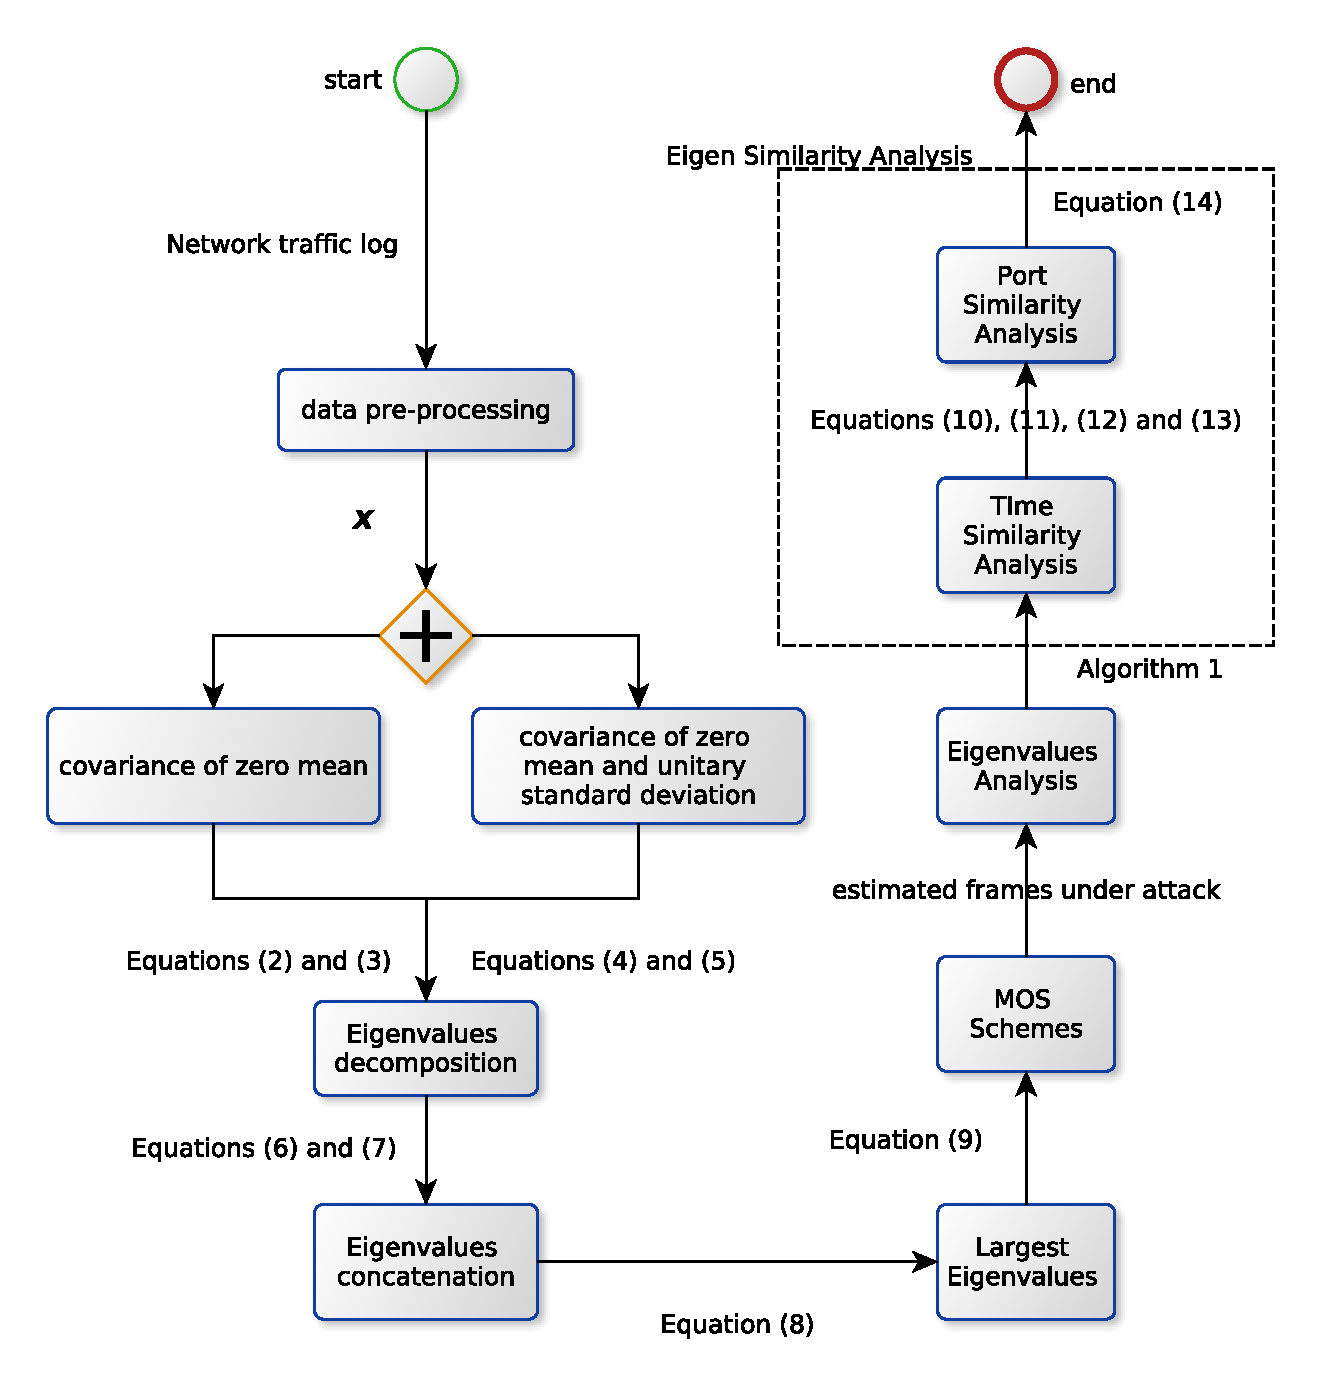
\includegraphics[width=11cm]{figures/mos_eigen_similarity.eps}
     \caption{Overview of The Framework for Detection and Identification of Network Attacks.}
     \label{fig:2.08}
\end{figure}

\subsection{Largest Eigenvalue by Time Frames}
\label{sec:2_prop_LargestEigenvaluebyTimeFrames}

The proposed attack detection algorithm starts by the data pre-processing of a network traffic log containing IP, ports and timestamp of senders and receivers. During this step, the desired information is extracted in order to classify and to count packets according to the origin and destination ports. Subsequently, this information is grouped by minutes and by time frames.

With the data grouped into $Q$ time frames, the framework considers the time variations of the matrix $\boldsymbol{X}^{(q)} \in \mathbb{R}^{M\times{N}}$, with $q = 1, \ldots, Q$, in order to detect the attack. 

According to flood and port scan attacks' behavior, flood attacks and port scan attacks can be characterized as covariance aware attack \citep{jin2004covariance} and correlation aware attack \citep{lakhina2005mining}, respectively. These characteristics are substantiated by the results obtained through the analysis based on sample covariance of zero mean variables and on covariance of zero mean and unitary standard deviation variables, described in Section \ref{sec:2_experimentalresults}, which shows that the main components of flood attacks are dominated by the variables with more variance and that the traffic associated with port scan attack does not generate many logs, however, it presents high covariance of zero mean and unitary standard deviation variables.

Therefore, to detect flood attacks, it is necessary to calculate the sample covariance matrix $\boldsymbol{\hat{R}}_{yy}^{(q)}$ of the zero mean samples given by

\begin{equation}
\label{eq:2.02}
\boldsymbol{y}_{m}^{(q)} = \boldsymbol{x}_{m}^{(q)} - \bar{\boldsymbol{x}}_{m}^{(q)}.
\end{equation}

The set of obtained vectors $\boldsymbol{y}_{m}^{(q)}$ composes the zero mean matrix $\boldsymbol{Y}^{(q)}$, then the sample covariance matrix $\boldsymbol{\hat{R}}_{yy}^{(q)}$ can be calculated as follows

\begin{equation}\label{eq:2.03}
\boldsymbol{\hat{R}}_{yy}^{(q)} = \frac{1}{N}\boldsymbol{Y}^{(q)}\boldsymbol{Y}^{(q)^{\rm T}}.
\end{equation}

For the detection of the port scan attack, the main components are not dominated by the variables with large variance. Moreover, the port scan traffic presents a highly correlated network traffic between the monitored ports. In order to exploit such structure, we compute the sample covariance $\boldsymbol{\hat{R}}_{zz}^{(q)}$ whose variables have zero mean and unitary standard deviation as follows

\begin{equation}
\label{eq:2.04}
\boldsymbol{z}_{m}^{(q)} = \frac{\boldsymbol{x}_{m}^{(q)} - \bar{\boldsymbol{x}}_{m}^{(q)}}{\boldsymbol{\sigma}_{m}^{(q)}}.
\end{equation}

The set of vectors $\boldsymbol{z}_{m}^{(q)}$ composes the matrix $\boldsymbol{Z}^{(q)}$, then the sample covariance matrix $\boldsymbol{\hat{R}}_{zz}^{(q)}$ can be calculated via 

\begin{equation}\label{eq:2.05}
\boldsymbol{\hat{R}}_{zz}^{(q)} = \frac{1}{N}\boldsymbol{Z}^{(q)}\boldsymbol{Z}^{(q)^{\rm T}}.
\end{equation}

Once the $\boldsymbol{\hat{R}}_{yy}^{(q)}$ and $\boldsymbol{\hat{R}}_{zz}^{(q)}$ have been obtained for flood and port scan detection, respectively, and since the next steps are the same for both sample covariance matrices, we refer to $\boldsymbol{\hat{R}}_{yy}$ and $\boldsymbol{\hat{R}}_{zz}$ as a matrix $\boldsymbol{\hat{R}}$. Therefore, the following step of the algorithm is the eigenvalue decomposition (EVD), calculated according to (\ref{eq:2.06}), in order to obtain the vector of eigenvalues $\boldsymbol{e}^{(q)}$ associated with each matrix, according to (\ref{eq:2.06}).

\begin{equation}\label{eq:2.06}
\boldsymbol{\hat{R}}^{(q)} = \boldsymbol{V}^{(q)}\boldsymbol{\Lambda}^{(q)}\boldsymbol{V}^{(q)^{\rm T}},
\end{equation}

\begin{equation}\label{eq:2.060}
\boldsymbol{e}^{(q)} = \rm diag(\boldsymbol{\Lambda}^{(q)}),
\end{equation}

where the operator diag$(\cdot)$ extracts the main diagonal of a matrix.

The eigenvalues should be sorted in descending order, i.e., $\lambda_{1}^{(q)} > \lambda_{2}^{(q)} > \lambda_{3}^{(q)} > ... > \lambda_{m}^{(q)}$. Therefore, the largest eigenvalue of the $q$-th time frame evaluated for the attack detect is given by $\lambda_{1}^{(q)}$.

The concatenation of the eigenvalues vector $\boldsymbol{e}^{(q)}$ for $q = 1, \ldots, Q$ is represented by

\begin{equation}\label{eq:2.07}
\boldsymbol{E} =
\begin{bmatrix}
  \lambda_1^{(1)} & \lambda_1^{(2)} & \lambda_1^{(3)} & \cdots & \lambda_1^{(Q)} \\
  \lambda_2^{(1)} & \lambda_2^{(2)} & \lambda_2^{(3)} & \cdots & \lambda_2^{(Q)} \\
  \lambda_3^{(1)} & \lambda_3^{(2)} & \lambda_3^{(3)} & \cdots & \lambda_3^{(Q)} \\
  \vdots & \vdots & \ddots & \vdots  \\
  \lambda_m^{(1)} & \lambda_m^{(2)} & \lambda_m^{(3)} & \cdots & \lambda_m^{(Q)} \\
\end{bmatrix}.
\end{equation}

Note that since $\lambda_1^{(q)} > \lambda_2^{(q)} > \lambda_3^{(q)} > \cdots > \lambda_{m-1}^{(q)} > \lambda_m^{(q)}$, then the first line of the matrix $\boldsymbol{E}$ contains the largest eigenvalues of each $q$-th time frame, which is the Greatest Eigenvalue Time
Vector (GETV) \cite{tenorio2013greatest}, denoted as 

\begin{equation}\label{eq:2.08}
\boldsymbol{e}_{\rm max} = [ \lambda_1^{(1)}, \lambda_1^{(2)} ... \lambda_1^{(Q)}]
\end{equation}

\subsection{MOS Schemes}
\label{sec:2_prop_MOSSchemes}

Traditionally the MOS schemes are applied for the eigenvalues of the vector $\boldsymbol{e}^{(q)}$. However, the goal here is to detect the variations of the eigenvalues for different values of $q$. Therefore, instead of using a certain $q$, the proposed approach applies MOS schemes for a vector of the largest eigenvalues of each $q$-th time frame, in order to identify variations and estimate the model order $\hat{d}$, which is the estimated number of time frames under attack. Therefore, $\boldsymbol{e}_{\rm max}$ is sorted in descending order, producing $\sim\boldsymbol{e}_{\rm max}$, that is used as input parameter for MOS schemes, according to $\hat{d} = \rm{MOS}(\sim\boldsymbol{e}_{\rm max})$. Note that some MOS schemes may also require the number of minutes that compose a time frame, as $\hat{d} = \rm{MOS}(\boldsymbol{e}_{\rm max},\emph{Q})$. For more information about MOS, we refer to the Appendix \ref{apx:a_mos}.

In our previous work \cite{tenorio2013greatest}, the accuracy of AIC, MDL, EDC, RADOI, EFT and SURE schemes are evaluated for synflood and port scan attack detection, showing that EDC and EFT are effective for detecting this kind of attacks. The present work extends that evaluation to also analyze the effectiveness of the listed MOS schemes for fraggle attack detection, as shown in Section \ref{sec:2_experimentalresults}.

\subsection{Eigenvalue Analysis}
\label{sec:2_prop_EigenvalueAnalysis}

After applying the MOS schemes to the vector $\sim\boldsymbol{e}_{\rm max}$, we obtain the estimate of the $\#\boldsymbol{X}$. For instance, in the case of fraggle, synflood and ports can, if $\hat{d} = 1$, , then $\#\boldsymbol{X} = 1$, which means that during the during the $Q$ time frames one attack is present. However, if $\hat{d} = 0$, then $\#\boldsymbol{X} = 0$, and this means that none of these attacks are present. Note that $\hat{d}$ can be greater than 1, indicating the presence of more than one attack.

In Subsection \ref{sec:2_prop_MOSSchemes}, we obtained only if $\hat{d} = 1$ or $\hat{d} = 0$. However, if $\hat{d} = 1$, the MOS schemes do not provide any information about the $q$-th time frame under attack. The identification of the $q$-th time frame under attack can be carried out through a eigenvalues analysis.

The largest eigenvalue analysis for estimating the $q$-th time frames that are under attack can be expressed according to Algorithm \ref{alg:2.01}, where $\rm{\boldsymbol{\hat{q}}}_{\rm max} \in \mathbb{R}^{\hat{d}}$ denotes a vector of the $q$-th time frames under attack, which is the $q$-th indexes corresponding to the $\hat{d}$ largest eigenvalues of $\boldsymbol{e}_{\rm max}$. Algorithm \ref{alg:2.01} initially identifies the largest value of $\boldsymbol{e}_{\rm max}$, according to Line 3 of Algorithm \ref{alg:2.01}, and its correspondent index, according to Line 7. Subsequently, the largest value is removed of $\boldsymbol{e}_{\rm max}$, according to Line 11 of Algorithm \ref{alg:2.01}, and a new iteration is performed until $\boldsymbol{e}_{\rm max} = []$.

\begin{algorithm}
	\label{alg:2.01}
	\SetAlgoLined
	\KwResult{$\rm{\boldsymbol{\hat{q}}}_{\rm max}$}
	Given $f = 1$\;
	\While{$f < \hat{d}$}{
		$q_{\rm value} = \operatorname*{argmax}_{\lambda}  \hspace{1 mm} \boldsymbol{e}_{\rm max}$\;
		$i = 1$\;
    	\While{$i < Q$}{
    		\If{$\boldsymbol{e}_{\rm max}^{(i)} == q_{\rm value}$}{
    			$\boldsymbol{\hat{q}}_{\rm max}^{(f)} = i$\;
    		}
    		$i = i + 1$\;
    	}
    	$\boldsymbol{e}_{\rm max} \rightarrow \boldsymbol{\hat{q}}_{\rm max}^{(f)}$\;
		$f = f + 1$\;
	}
	\caption{Detection of Time Frames Under Attack}
\end{algorithm}

After the estimation of the $\rm{\boldsymbol{\hat{q}}}_{\rm max}$ time frames under attack, it is necessary to obtain more details of the detected Attacks, such as the $n$-th minutes when the attacks happened and the $m$-th network ports that were attacked. To deal with this problem, the adoption of a similarity analysis between legitimate traffic and the traffic of time frames estimated as under attack is evaluated, analyzing the effectiveness of cosine similarity to highlight abnormalities inserted by network traffic attacks. 

\subsection{Eigen Similarity Analysis}
\label{sec:2_prop_EigenSimilarityAnalysis}

Cosine similarity calculates the cosine of the angle between two vectors, which represents the similarity of values between the selected vectors. Therefore, cosine similarity can be used to evaluate the variation of the most significant eigenvectors of $\boldsymbol{V}^{(q)}$ against the most significant eigenvectors of time frame detected as under attack, to analyze similarity changes into the most significant eigenvectors caused by the insertion of anomalous traffic \cite{Lee2013}. 

This subsection describes the proposed eigen similarity analysis for detailed attack identification, in complement to the attack estimation carried out through MOS schemes and eigenvalue analysis. In Subsection \ref{sec:2_prop_TimeSimilarityAnalysis} we present the eigen similarity analysis for identification of time under attack. Next, in Subsection \ref{sec:2_prop_PortSimilarityAnalysis}, we show how to apply the eigen similarity analysis in order to identify network ports under attack.

\subsubsection{Time Similarity Analysis}
\label{sec:2_prop_TimeSimilarityAnalysis}
% ToDo
For eigen similarity analysis, we evaluate the cosine similarity in order to identify lacks of similarity between legitimate and malicious traffic, as follows

\begin{equation}\label{eq:2.11}
s_n = \frac{\abs{\boldsymbol{v}^{(q)} \cdot \boldsymbol{v}_{(n)}^{(q)}}}{\norm{\boldsymbol{v}^{(q)}}\norm{\boldsymbol{v}_{(n)}^{(q)}}},
\end{equation}
where $s_n$ denotes the absolute similarity degree of the $n$-th minute, $\boldsymbol{v}^{(q)}$ is the most significant eigenvectors of a selected set of minutes without network attack, according the attack detection described by Algorithm \ref{alg:2.01}, and $\boldsymbol{v}_{(n)}^{(q)}$ is the most significant eigenvectors obtained after append each target $n$-th minute of traffic that needs the identification of flood and port scan attacks.

The most significant eigenvector $\boldsymbol{v}^{(q)}$, of a time frame $q$ without attack, can be computed from (\ref{eq:2.06}) and selected according to the eigenvector of the largest eigenvalue $\lambda_1^{(q)}$, which is the principal component of the selected time frame $q$. The same calculation shall be performed in order to obtain the target eigenvectors $\boldsymbol{v}_{(n)}^{(q)}$, calculated from the time frame without attack appended by selected minutes of a time frame estimated as under attack.

Therefore, the reference eigenvectors $\boldsymbol{v}^{(q)}$ is calculated from the traffic without attack, in a time frame $q$ composed of $Q$ minutes of legitimate network traffic, estimated as normal by Algorithm \ref{alg:2.01}. For the detailed attack identification, each $\boldsymbol{x}^{(\hat{q})}_{(n)}$ vector of each $n$-th minutes of the estimated $\rm{\boldsymbol{\hat{q}}}_{\rm max}$ time frames shall be individually appended into $\boldsymbol{X}^{(q)}$, as represented by

\begin{equation}\label{eq:2.12}
\boldsymbol{X}_{n} = \{\boldsymbol{X}^{(q)} | \boldsymbol{x}^{(\hat{q})}_{(n)}\}.
\end{equation}

Subsequently, the resultant $\boldsymbol{X}_{(n)}$ is used to obtain $\boldsymbol{v}_{(n)}^{(q)}$, through (\ref{eq:2.06}), for calculating the similarity degree $s_n$, ranging from 0 to 1, for each $n$-th minute. The $s_n$ denotes the absolute similarity degree of the $n$-th minute in comparison to a well-known traffic without attack, detected through MOS schemes and eigenvalue analysis.

We propose three approaches for eigen similarity analysis, which are the incremental, the individual and the incremental individualized.

The incremental approach for eigen similarity analysis is based on the incremental appending of network traffic into $\boldsymbol{X}^{(q)}$, where the first evaluation is based on (\ref{eq:2.12}) and the subsequent evaluations are based on (\ref{eq:2.13}), that denotes the appending of the $n$-th minute $\boldsymbol{x}^{(\hat{q})}_{(n)}$ into $\boldsymbol{X_n}$. The incremental approach repeats the Equation \ref{eq:2.13} while $n \leq N$ and compute $\boldsymbol{v}^{(q)}$, $\boldsymbol{v}_{(n)}^{(q)}$ and the Equation \ref{eq:2.11} for each increment.

\begin{equation}\label{eq:2.13}
\boldsymbol{X}_{n} = \{\boldsymbol{X}_{n} | \boldsymbol{x}^{(\hat{q})}_{(n)}\},
\end{equation}

Figure \ref{fig:2.08} illustrates the network traffic selection for the incremental approach of eigen similarity analysis, where the $\boldsymbol{X}^{(1)}$ is chosen as reference for similarity analysis of the $m$-th minutes of the time frame $q=3$, where one network attack was previously detected by Algorithm \ref{alg:2.01}. 

%TODO - fix figure that shows s_n > l where should the inverse
\begin{figure}[h!]
     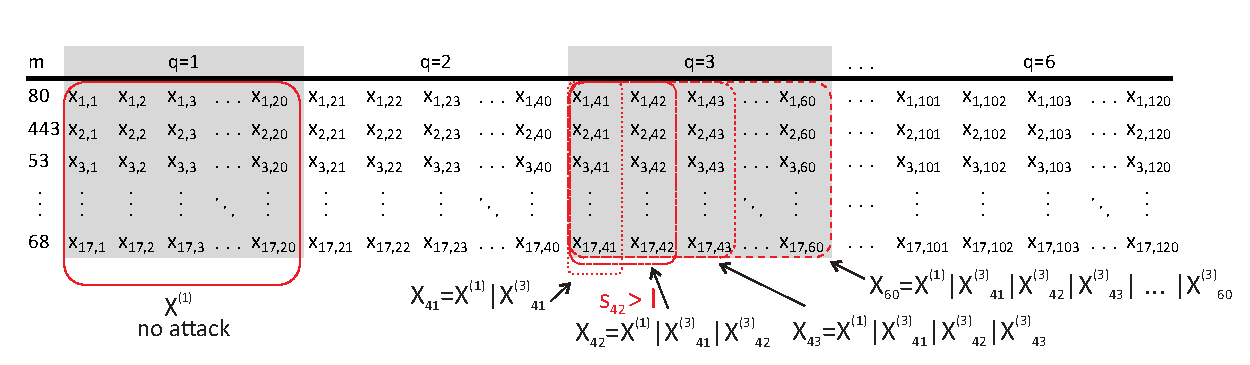
\includegraphics[width=15cm]{figures/incremental.eps}
     \caption{Traffic selection for incremental approach.}
     \label{fig:2.08}
\end{figure}

For the scenario depicted by Figure \ref{fig:2.08}, the eigen similarity analysis starts at $\boldsymbol{x}^{(3)}_{(41)}$ and is incrementally performed until $\boldsymbol{x}^{(3)}_{(60)}$, in order to calculate the $s_n$. We assume that $s_n < l$ means an attack identification, according the anomaly on similarity of $s_n$ compared to a defined limiar $l$. 

Therefore, after obtaining the most significant eigenvector $\boldsymbol{v}^{(q)}$ and the target eigenvectors $\boldsymbol{v}_{(n)}^{(q)}$ for eigen similarity analysis, the $s_n$ is calculated according to (\ref{eq:2.11}). If $s_n = 1$, then the two eigenvectors are completely similar and no anomaly is detected. Smaller values of $s_n$ mean less similarity and can indicate an anomaly if $s_n < l$, what denotes that a network attack is identified during the $n$-th minute. 

The Equation \ref{eq:2.14} shows how the $s_n$ of each $n$-th minute shall be compared with the threshold $l$ to evaluate if a attack is identified, where

\begin{equation}\label{eq:2.14}
  \boldsymbol{\hat{n}_{(n)}}=\left\{
  \begin{array}{@{}ll@{}}
    1, & \text{if}\ s_n < l \\
    0, & \text{otherwise}
  \end{array}\right.,
\end{equation}
and $\boldsymbol{\hat{n}}_{(n)}$ denotes a vector of $n$-th minutes detected as under attack.

The eigen similarity analysis can also be applied by means of the individual approach, where each $n$-th minute must be individually appended into $\boldsymbol{X}^{(q)}$, as shown by Figure \ref{fig:2.09}. In the individual approach there is no incremental appending, therefore only individual $n$-th minute are appended to $\boldsymbol{X_n}$, according to \ref{eq:2.12}, in order to compute $\boldsymbol{v}^{(q)}$, $\boldsymbol{v}_{(n)}^{(q)}$ and the Equation \ref{eq:2.11} for individual $n$-th minute.

%TODO - fix figure that shows s_n > l where should the inverse
\begin{figure}[h!]
     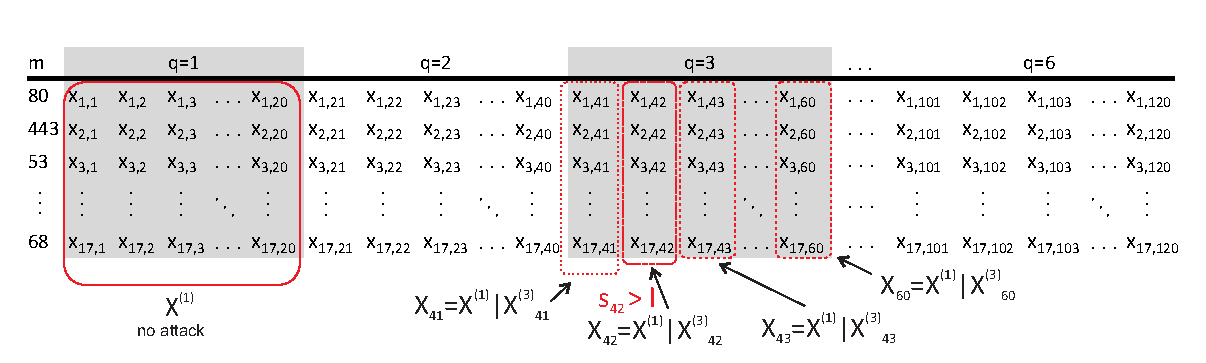
\includegraphics[width=15cm]{figures/individualized.eps}
     \caption{Traffic selection for individual approach.}
     \label{fig:2.09}
\end{figure}

The incremental and the individual approaches can be combined to obtain the incremental individualized approach, where each minute is incrementally appended into the selected $\boldsymbol{X}^{(q)}$ for obtaining $\boldsymbol{v}_{(n)}^{(q)}$ to compute similarity analysis of the $n$-th minute, until detect the first $n$-th minute under attack, i.e. $s_n < l$. Subsequently, $\boldsymbol{X}_{n-1}$ becomes the new reference of traffic without network attack and each subsequent minute must have its similarity individually evaluated, as shown in Figure \ref{fig:2.02}.

%TODO - fix figure that shows s_n > l where should the inverse
\begin{figure}[h!]
     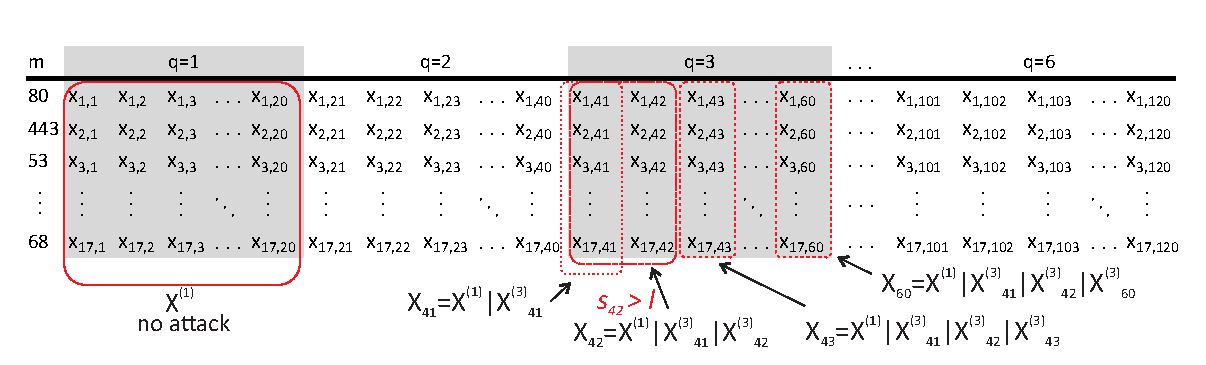
\includegraphics[width=15cm]{figures/incremental_individualized.eps}
     \caption{Traffic selection for incremental individualized approach.}
     \label{fig:2.02}
\end{figure}

The incremental similarity analysis followed by individual analysis after an attack detection allows to identify the attack period, highlighting the first and last time under attack. This identification is possible due to the variation of the most significant eigenvectors, which becomes more significant when compared a traffic under attack against a traffic with no attack, according to results which are discussed in Section \ref{sec:2_experimentalresults}.

\subsubsection{Port Similarity Analysis}
\label{sec:2_prop_PortSimilarityAnalysis}

Given $\boldsymbol{\hat{n}}$, which is the set of $n$-th minutes under attack, it is still necessary to obtain more details about the identified network attack, such as the network ports that are attacked during each $n$-th minute identified as under attack. Hence, it is also applied the cosine similarity analysis to identify variation of the most significant eigenvectors, caused by the insertion of anomalous network traffic by a selected $m$-th port during a $n$-th minute. 

For detection of ports under attack, the last most significant eigenvectors without attack $\boldsymbol{v}^{(q)}$ shall be used as reference for similarity analysis against the $\boldsymbol{v}_{(n)}^{(q)}$ identified as under attack, and evaluate individually the cosine similarity of each $m$-th port of all $\boldsymbol{\hat{n}}$ minutes. Therefore, $\boldsymbol{v}^{(q)}$ should be calculated from the last $\boldsymbol{X}^{(q)}$ time frame without attack, and $\boldsymbol{v}_{(m,\hat{n})}$ should be calculated from the same traffic appended of all $n$-th minutes until the identified minute under attack, denoted as $\boldsymbol{X}_n$. 

For similarity analysis, each $m$-th port of the last $n$-th minute of $\boldsymbol{X}_n$, denoted as $x_{(m,n)}$, shall be individually replaced by the traffic of the evaluated $m$-th port of the $\hat{n}$-th minute under attack, denoted as $x^{(\hat{q})}_{(m,\hat{n})}$, in order to identify significant variation on similarity caused by the traffic of the $m$-th port. 

This approach for detection of ports under attack via similarity analysis is given by

\begin{equation}\label{eq:2.15}
  \left\{
  \begin{array}{@{}ll@{}}
    x_{(m,n)} = x^{(\hat{q})}_{(m,\hat{n})} \\
    \\
    s_{m,\hat{n}} = \frac{\abs{\boldsymbol{v}^{(q)} \cdot \boldsymbol{v}_{(m,\hat{n})}}}{\norm{\boldsymbol{v}^{(q)}}\norm{\boldsymbol{v}_{(m,\hat{n})}}},
  \end{array}\right.
\end{equation}
where $x^{(\hat{q})}_{(m,\hat{n})}$ denotes the $m$-th port of the selected $n$-th minute and $q$-th time frame identified as under attack and $x_{(m,n)}$ denotes the $m$-th port of the last $n$-th minute of $\boldsymbol{X}_n$, which is used to calculate the $\boldsymbol{v}_{(m,\hat{n})}$ most significant eigenvectors that contains the traffic of the $m$-th port of the $\hat{n}$-th minute identified as under attack.

Once $\boldsymbol{v}^{(q)}$ and $\boldsymbol{v}_{(m,\hat{n})}$ are obtained, then the $s_{m,\hat{n}}$ similarity degree can be calculated in order to identify if the traffic replacement highlights the adition of anomalous traffic by the evaluated $m$-th port during the $\hat{n}$-th minute previously identified as under attack. 

This procedure should be repeated for each $m$-th target port of $\boldsymbol{\hat{n}}$, in order to individually identify the network ports under attack during each $\hat{q}$-th time frame.


\section{Experiments and Results}
\label{sec:2_experimentalresults}

This section presents the performed experiments and the acquired results for the Eigensim. First, in Section \ref{sec:2_AnalyzedScenario}, the experimental scenario adopted in the evaluation is summarized. Then, Section \ref{sec:2_largesteigenvaluesanalysis} shows the results of the largest eigenvalue analysis by time frames for the experimental scenario. In Section \ref{sec:2_MOSSchemesEvaluation} are described the results of the evaluated MOS schemes for attack detection in the simulated data set. Section \ref{sec:2_EigenvalueAnalysis} presents the results of the eigenvalue analysis for identification of time frames under attack, Section \ref{sec:2_EigenSimilarityAnalysis} shows the results of similarity analysis for detailed flood and port scan identification for the experimental scenario. Section \ref{sec:2_DarpaEvaluation} presents the results of the largest eigenvalue analysis, model order selection and the eigenvalue analysis for flood and probe attack detection in the DARPA 1998 data set.

\subsection{Experimental Scenario}
\label{sec:2_AnalyzedScenario}

This experiment consider a simulated scenario of a real network monitored during 120 minutes, that are separated into six time frames of twenty minutes. Therefore, as the time of each sampling period is one minute, then $N = 20$. For each time frame $q$, a traffic matrix $\boldsymbol{X}^{(q)} \in \mathbb{R}^{17 \times 20}$ was obtained, as well as a covariance $\boldsymbol{\hat{R}}_{yy}^{(q)} \in \mathbb{R}^{17 \times 17}$ (calculated via (\ref{eq:2.03})) and a sample covariance matrix $\boldsymbol{\hat{R}}_{zz}^{(q)} \in \mathbb{R}^{17x17}$, assuming that $q = 1, 2, 3, 4, 5$ and $6$. 

The simulation started at 21:00h, the first time frame was from 21:00h until 21:20h ($q = 1$), the second was from 21:20h until 21:40h ($q = 2$), the third was from 21:40h to 22:00h ($q = 3$), the fourth was from 22:00h until 22:20h ($q = 4$), the fifth was from 22:20h until 22:40h ($q = 5$), and finally, the sixth was from 22:40h until 23.00h ($q = 6$). During the simulation, the victim made legitimate access, and the attacker performed the following attacks: at 21:54h ($q = 3$) was performed a port scan, at the interval ranging from 22:10h to 22:20h ($q = 4$) a synflood attack was simulated, and at the interval from 22:30h to 22:40h ($q = 5$) a fraggle attack was performed.

\subsection{Largest Eigenvalues Analysis}
\label{sec:2_largesteigenvaluesanalysis}

For the evaluation of MOS Schemes accuracy for flood and port scan detection, the framework defines that it is necessary to obtain the largest eigenvalue of each time frame, through eigen decomposition from a covariance of zero mean variables or covariance matrix of zero mean and unitary standard deviation variables, calculated from the evaluated traffic, as described in Section \ref{sec:2_prop_getv}. Through eigenvalue analysis of traffic with flood or port scan attacks, it is possible to visualize a significant difference between the largest eigenvalues and the remain eigenvalues, which can indicate a relationship between an outlier and time frames under attack.

\begin{figure}[h!]
	\centering
     \includegraphics[width=11cm]{figures/eigenvalues_synflood.eps} 
     \caption{Eigenvalues of the sample covariance matrix (synflood).}
     \label{fig:2.10}
\end{figure}

Figure \ref{fig:2.10} depicts the eigenvalues calculated from sample covariance matrix of the network traffic used to evaluate the synflood attack identification. In Figure \ref{fig:2.10}, the largest eigenvalue related to the simulated synflood attack ($q = 4$) stands out significantly from the other eigenvalues.

Figure \ref{fig:2.11} illustrates the eigenvalues calculated from sample covariance matrix of the matrix used for fraggle attack detection. In Figure \ref{fig:2.10}, the largest eigenvalue related to the simulated synflood attack ($q = 5$) stands out significantly from the other eigenvalues, in accordance with the result shown in Figure \ref{fig:2.10} for the synflood attack analysis.

\begin{figure}[h!]
	\centering
     \includegraphics[width=11cm]{figures/eigenvalues_fraggle.eps}
     \caption{Eigenvalues of the sample covariance matrix (fraggle).}
     \label{fig:2.11}
\end{figure}

Figure \ref{fig:2.12} depicts the eigenvalues calculated from covariance matrix of zero mean and unitary standard deviation variables, of the network traffic matrix evaluated for port scan detection. As analyzed for the synflood and fraggle attacks, note that the largest eigenvalue, related to this attack ($q = 3$), stands out significantly from the others eigenvalues.

\begin{figure}[h!]
	\centering
     \includegraphics[width=11cm]{figures/eigenvalues_portscan.eps}
     \caption{Eigenvalues of the covariance matrix of zero mean and unitary standard deviation (port scan).}
     \label{fig:2.12}
\end{figure}

Table \ref{tab:2.03} presents the values of the largest eigenvalues of each time frame $q$-th for port scan, synflood and fraggle detection. 

\begin{table}[h!]
  \centering
  % \footnotesize
  \caption{Largest Eigenvalue related to attacks detection}
  \label{tab:2.03}
  \begin{tabular}{ c c c c c }
	\toprule
	\multirow{3}{*}{\textbf{Time Frame} $q$} &\multicolumn{4}{c }{\textbf{Vectors GETV}}\\ 
			\hhline{~----}
		&\textbf{Detection of}	 &\textbf{Detection of}	 &\textbf{Detection of}	 &\textbf{Detection of}\\
		&\textbf{\emph{synflood/fraggle}}	 &\textbf{\emph{synflood}}	 &\textbf{\emph{fraggle}}	 &\textbf{\emph{port scan}}\\
	\midrule
	1 &1887545 &1887545 &1887545 &2,0734 \\
	2 &2341327 &2341327 &2341327 &2,1451 \\
	3 &3213867 &3213867 &3213867 &10,0718 \\
	4 &133238294 &133238294 &731229 &2,1620 \\
	5 &92384021611 &6367983 &92384021611 &2,4253 \\
	6 &708335 &708335 &708335 &1,7948 \\
    \bottomrule
  \end{tabular}
\end{table}

In Table \ref{tab:2.03}, note the significant variation of the eigenvalues associated with attacks, in comparison to the others. At $q = 4$, where the synflood attack occurred, the maximum eigenvalue obtained is approximately 21 times larger than the second one. At $q = 5$, where the fraggle attack occurred, the maximum eigenvalue obtained is about 29,000 times larger than the second one. At $q = 3$, where the port scan attack occurred, the maximum eigenvalue obtained is approximately 4 times larger than the second one. In the last case, for port scan attack detection, although the largest eigenvalue presented no too large variance to the second one, if compared to synflood or fraggle attacks, it clearly deviates from the remaining largest eigenvalues.

These results highlight that all $q$-th time frames where a network attack was simulated, present high significant variance between the largest eigenvalue and the remaining eigenvalues, obtained from sample covariance matrix, for flood detection, or from covariance matrix of zero mean and unitary standard deviation variables, for port scan detection. Therefore, we propose to apply the vector of the largest eigenvalues to MOS schemes in order to evaluate their accuracy for identification of time frames under attack, motivated by the fact that it is relevant to apply MOS schemes to automate the attack detection process, taking into account the characteristics of the evaluated eigenvalues.

\subsection{MOS Schemes Evaluation}
\label{sec:2_MOSSchemesEvaluation}

In \cite{tenorio2013greatest}, we evaluate the accuracy of AIC, MDL, EDC, RADOI, EFT and SURE MOS schemes \cite{da2009comparison,tenorio2013greatest} for synflood and port scan attack detection. In this work we extend that evaluation for fraggle attack detection, applying the same schemes to fraggle attack detection over the traffic presented in Section \ref{sec:2_datamodel}, as results shown in Table \ref{tab:2.04}.

\begin{table}[h!]
  \centering
  % \scriptsize
  \caption{MOS schemes applied to port scan and flood detection}
  \label{tab:2.04}
  \begin{tabular}{ c c c c c c c c }
	\toprule
	\multirow{2}{*}{\textbf{Type of analysis} $q$} &\multicolumn{6}{c}{\textbf{MOS schemes (estimated model order $\hat{d}$)}} &{\textbf{(d)}}\\ 
			\hhline{~------~}
		&\textbf{AIC} &\textbf{MDL} &\textbf{EDC} &\textbf{RADOI} &\textbf{EFT} &\textbf{SURE}\\
	\midrule
	Detection of synflood \\(presence of attack) &2 &1 &\textbf{1} &5 &\textbf{1} &4 &\textbf{1} \\
	Detection of synflood \\(absence of attack) &1 &1 &\textbf{0} &1 &\textbf{0} &3 &\textbf{0} \\
	\midrule
	Detection of fraggle \\(presence of attack) &1 &1 &\textbf{1} &5 &\textbf{1} &4 &\textbf{1} \\
	Detection of fraggle \\(absence of attack) &1 &1 &\textbf{0} &1 &\textbf{0} &3 &\textbf{0} \\
	\midrule
	Detection of port scan \\(presence of attack) &1 &1 &\textbf{1} &1 &\textbf{1} &9 &\textbf{1} \\
	Detection of port scan \\(absence of attack) &0 &0 &\textbf{0} &1 &\textbf{0} &1 &\textbf{0} \\
	\midrule
	Detection of synflood/fraggle \\(presence of attack) &2 &2 &\textbf{2} &5 &\textbf{2} &5 &\textbf{2} \\
	Detection of synflood/fraggle \\(absence of attack) &1 &1 &\textbf{0} &1 &\textbf{0} &3 &\textbf{0} \\
    \bottomrule
  \end{tabular}
\end{table}

Note that $\hat{d} = 1$, if there is attack, while $\hat{d} > 1$ indicates more than one attack. An example of this could be seen for attack detection via EFT for traffic containing synflood and fraggle attacks, showing $\hat{d} = 2$, which indicates the presence of two attacks, as expected by the ground truth values $d$ of Table \ref{tab:2.04}. 

In Table \ref{tab:2.04}, two MOS schemes outperforms from the others, which are EDC and EFT. Efficient Detection Criterion (EDC) and Exponential Fitting Test (EFT) are the most effective schemes, correctly estimating the number of attacks in comparison to the expected values for effective attack detection, as defined by the column of real values in Table \ref{tab:2.04}. The AIC and MDL schemes are satisfactory only for port scan detection, however SURE and RADOI schemes did not show effective results for port scan or flood detection.

Although EDC and EFT presented the same accuracy on the evaluation, the EDC scheme requires less processing time than EFT, which is an important criteria to select EDC as the MOS scheme for flood and port scan detection on the remain experiments.

According to Table \ref{tab:2.04}, EDC and EFT estimated correctly the number of attacks of a time frame vector, indicating that occurred $\hat{d}$ network attacks, but not providing additional details, what highlights the necessity of complementary approaches in order to estimate the time and ports under attack. Hence, we propose apply eigen analysis to estimate the $q$-th time frames under attack and eigen similarity analysis to estimate the minutes and ports under attack.

\subsection{Eigenvalue Analysis}
\label{sec:2_EigenvalueAnalysis}

According to the results presented in Section \ref{sec:2_largesteigenvaluesanalysis}, the largest eigenvalue stands out significantly from the others eigenvalues of an evaluated $q$-th time frame. This behavior can also be observed in the largest eigenvalues analysis, according to results presented in Table \ref{tab:2.03}, where it is possible to observe that the $\hat{d}$ largest eigen values of the time frames under attacks stand out significantly from the others largest eigenvalues. 

Therefore, we conclude that the $\hat{d}$ largest eigenvalues correspond to the respective $q$-th time frames under attack, which is denoted by $\rm{\boldsymbol{\hat{q}}}_{\rm max}$ and can be calculated according to Algorithm \ref{alg:2.01}.

\subsection{Eigen Similarity Analysis}
\label{sec:2_EigenSimilarityAnalysis}

This work proposes applying eigen similarity analysis to detect time and ports under attack, from each $q$-th time frames under attack defined by $\rm{\boldsymbol{\hat{q}}}_{\rm max}$. Hence, the proposed framework is applied to the time frames where $q=3$, $q=4$ and $q=5$ to respectively evaluate its effectiveness for port scan, synflood and fraggle attack detection.

\subsubsection{Time Analysis}
\label{sec:2_TimeAnalysis}

Three approaches were evaluated for eigen similarity analysis: incremental, individual and incremental individualized approaches. For the incremental individualized approach, each minute is incrementally appended into the selected $\boldsymbol{X}^{(q)}$ for obtaining $\boldsymbol{v}_{(n)}^{(q)}$ to similarity analysis of the $n$-th minute, until detect the first $n$-th minute under attack. Subsequently, $\boldsymbol{X}_n$ became the new reference of traffic without network attack and each subsequent minute must have its similarity individually evaluated. For the incremental approach, each $n$-th minute must be incrementally appended into $\boldsymbol{X}^{(q)}$, for obtaining the next eigenvectors $\boldsymbol{v}_{(n)}^{(q)}$ for individual time similarity analysis. For the individual approach, each $n$-th minute must be individually appended into $\boldsymbol{X}^{(q)}$, without incremental append, but doing individual appended into $\boldsymbol{X}^{(q)}$ for obtaining the next eigenvectors $\boldsymbol{v}_{(n)}^{(q)}$ for individual similarity analyis.

Table \ref{tab:2.05} presents the results of the evaluation of three approaches for similarity analysis of eigenvectors for port scan detection.

\begin{table}[h!]
  \centering
  \footnotesize
  \caption{Eigen Similarity Analysis for Port Scan Detection}
  \label{tab:2.05}
  \begin{tabular}{ c c c c c c }
	\toprule
	\multirow{2}{*}{\textbf{Time Frame} $q$} &\multirow{2}{*}{\textbf{Time} $n$}   &\multicolumn{3}{c}{\textbf{Similarity Analysis}} &\multirow{2}{*}{\textbf{Ground Truth}}\\ 
			\hhline{~~---~}
			& &\textbf{Incremental Individualized} &\textbf{Incremental} &\textbf{Individual}\\
	\midrule
	3 &1 &0.9946 &0.9946 &0.9946 &no \\
	3 &2 &0.9934 &0.9934 &0.9999 &no \\
	3 &3 &0.9912 &0.9912 &0.9999 &no \\
	3 &4 &0.9888 &0.9888 &0.9999 &no \\
	3 &5 &0.9856 &0.9856 &0.9998 &no \\
	3 &6 &0.9840 &0.9840 &0.9999 &no \\
	3 &7 &0.9824 &0.9824 &1.0000 &no \\
	3 &8 &0.9794 &0.9794 &0.9999 &no \\
	3 &9 &0.9673 &0.9673 &0.9926 &no \\
	3 &10 &0.9674 &0.9674 &0.9997 &no \\
	3 &11 &0.9733 &0.9733 &0.9993 &no \\
	3 &12 &0.9702 &0.9702 &0.9993 &no \\
	3 &13 &0.9677 &0.9677 &0.9999 &no \\
	3 &14 &0.9646 &0.9646 &0.9998 &no \\
	3 &15 &0.0216 &0.0216 &0.0276 &yes \\
	3 &16 &0.9621 &0.0209 &1.0000 &no \\
	3 &17 &0.9611 &0.0199 &0.9998 &no \\
	3 &18 &0.9612 &0.0191 &0.9999 &no \\
	3 &19 &0.9613 &0.0186 &0.9998 &no \\
	3 &20 &0.9638 &0.0190 &1.0000 &no \\
    \bottomrule
  \end{tabular}
\end{table}

Table \ref{tab:2.05} shows the evaluation of the time frame $q=3$, when the port scan attack was simulated, considering the incremental individualized, incremental and individual approaches for eigen similarity analysis. According to the presented results, it is possible to observe the high similarity between network traffic without attack, which was larger than 0.9610 for all evaluated cases, and emphasize the expressive low similarity when it was evaluated the traffic with the simulated port scan attack ($n=15$), which was lower than 0.0276 for all evaluated approaches.

Comparing the approaches for similarity analysis, it is possible to observe that all approaches highlight the low similarity when evaluated the traffic under attack. However, the incremental approach figured out low similarity for times without attack, where $n=16, 17, 18, 19, 20$, what indicates that the incremental approach can produce false positive results. This behavior occurs because the incremental approaches appends all selected traffic into the reference traffic for comparison against the original reference traffic, what makes more evident the first lack of similarity but reduces the changing detection capability after an attack detection.

Table \ref{tab:2.06} presents the results of the evaluation of the similarity analysis of eigenvectors for synflood detection. It shows the evaluation of the time frame $q=4$, when the synflood attack is simulated, considering the incremental individualized, incremental and individual approaches for eigen similarity analysis. According to the results, it is possible to observe the high similarity between network traffic without attack, which is larger than 0.9907 for all evaluated cases, and emphasize the expressive low similarity when evaluated the traffic with synflood attack (between $n=11$ and $n=20$), which is lower than 0.1244 for all evaluated approaches.

\begin{table}[h!]
  \centering
  \footnotesize
  \caption{Eigen Similarity Analysis for Synflood Detection}
  \label{tab:2.06}
  \begin{tabular}{ c c c c c c }
	\toprule
	\multirow{2}{*}{\textbf{Time Frame} $q$} &\multirow{2}{*}{\textbf{Time} $n$}   &\multicolumn{3}{c}{\textbf{Similarity Analysis}} &\multirow{2}{*}{\textbf{Ground Truth}}\\ 
			\hhline{~~---~}
			& &\textbf{Incremental Individualized} &\textbf{Incremental} &\textbf{Individual}\\
	\midrule
	4 &1 &1.0000 &1.0000 &1.0000 &no \\
	4 &2 &0.9999 &0.9999 &1.0000 &no \\
	4 &3 &0.9997 &0.9997 &0.9999 &no \\
	4 &4 &0.9998 &0.9998 &1.0000 &no \\
	4 &5 &0.9965 &0.9965 &0.9908 &no \\
	4 &6 &0.9975 &0.9975 &1.0000 &no \\
	4 &7 &0.9977 &0.9977 &1.0000 &no \\
	4 &8 &0.9980 &0.9980 &1.0000 &no \\
	4 &9 &0.9987 &0.9987 &0.9999 &no \\
	4 &10 &0.9991 &0.9991 &1.0000 &no \\
	4 &11 &0.0085 &0.0085 &0.0284 &yes \\
	4 &12 &0.0162 &0.0120 &0.0343 &yes \\
	4 &13 &0.0248 &0.0158 &0.0427 &yes \\
	4 &14 &0.1243 &0.0185 &0.1041 &yes \\
	4 &15 &0.0082 &0.0162 &0.0103 &yes \\
	4 &16 &0.0404 &0.0070 &0.0580 &yes \\
	4 &17 &0.0397 &0.0007 &0.0573 &yes \\
	4 &18 &0.0408 &0.0042 &0.0584 &yes \\
	4 &19 &0.0408 &0.0079 &0.0584 &yes \\
	4 &20 &0.0477 &0.0092 &0.0757 &yes \\
    \bottomrule
  \end{tabular}
\end{table}

The incremental approach produces better results if compared with other evaluated approaches, with lower values and maximum of 0.0185 for times under attack, but this approach presents change detection limitation after the first outlier of similarity, in accordance to the results shown in Table \ref{tab:2.05} for port scan detection. 

Comparing the incremental individualized and the individual approaches for eigen similarity analysis, it is possible to observe that the incremental individualized approach obtain lowest values for almost all cases, except for the time $n=14$, where incremental individualized approach identified a larger similarity than the individual approach. The incremental individualized appends information about each evaluated traffic, therefore it incorporates traffic behaviors that can reduce the outlier capability detection, as occurred for the time $n=14$.

Table \ref{tab:2.07} presents the results of the eigen similarity analysis evaluation for fraggle detection.

\begin{table}[h!]
  \centering
  \footnotesize
  \caption{Eigen Similarity Analysis for Fraggle Detection}
  \label{tab:2.07}
  \begin{tabular}{ c c c c c c }
	\toprule
	\multirow{2}{*}{\textbf{Time Frame} $q$} &\multirow{2}{*}{\textbf{Time} $n$}   &\multicolumn{3}{c}{\textbf{Similarity Analysis}} &\multirow{2}{*}{\textbf{Ground Truth}}\\ 
			\hhline{~~---~}
			& &\textbf{Incremental Individualized} &\textbf{Incremental} &\textbf{Individual}\\
	\midrule
	5 &1 &1.0000 &1.0000 &1.0000 &no \\
	5 &2 &0.9999 &0.9999 &1.0000 &no \\
	5 &3 &1.0000 &1.0000 &1.0000 &no \\
	5 &4 &0.9999 &0.9999 &1.0000 &no \\
	5 &5 &0.9993 &0.9993 &0.9997 &no \\
	5 &6 &0.9993 &0.9993 &0.9997 &no \\
	5 &7 &0.9994 &0.9994 &1.0000 &no \\
	5 &8 &0.9995 &0.9995 &1.0000 &no \\
	5 &9 &0.9995 &0.9995 &1.0000 &no \\
	5 &10 &0.9995 &0.9995 &1.0000 &no \\
	5 &11 &0.0031 &0.0031 &0.0021 &yes \\
	5 &12 &0.0019 &0.0025 &0.0009 &yes \\
	5 &13 &0.0030 &0.0026 &0.0020 &yes \\
	5 &14 &0.0030 &0.0027 &0.0020 &yes \\
	5 &15 &0.0030 &0.0028 &0.0020 &yes \\
	5 &16 &0.0012 &0.0025 &0.0002 &yes \\
	5 &17 &0.0030 &0.0026 &0.0020 &yes \\
	5 &18 &0.0030 &0.0026 &0.0020 &yes \\
	5 &19 &0.0030 &0.0027 &0.0020 &yes \\
	5 &20 &0.0069 &0.0023 &0.0083 &yes \\
    \bottomrule
  \end{tabular}
\end{table}

For fraggle attack detection, the lack of similarity between legitimate and malicious traffic was more evident than for the evaluation of synflood and port scan detection. This behavior can be explained by the number of packets generated through the fraggle attack simulation, that was significantly larger than the number of packets generated during the synflood simulation. Considering the three approaches, the largest value for times under attack was 0.0083, while the shortest value for times without attacks was 0.9993. 

Therefore, considering the evaluation for port scan, synflood and fraggle detection, the incremental approach can produce false positive results, while the individual and incremental individualized approaches produce quite similar results, even though the individual approach be more simple and require less memory and processing time.

These results highlight the capability of change detection based on similarity between legitimate and malicious traffic from flood or port scan attacks, by means of a subspace learned via Eigenvalue Value Decomposition and Model Order Selection,
endorsing the effectiveness and safety for adoption of threshold for attack detection through eigen similarity analysis. Moreover, these results answer positively the question $Q_1$, what rejects the null hypothesis  $H_{0sub}$ and confirms the alternative
hypothesis $H_{1sub}$.

\subsubsection{Port Analysis}
\label{sec:2_PortAnalysis}

Given $\hat{N}$, which is the set of estimated $n$-th minutes under attack, it is possible to apply cosine similarity analysis to identify variation of the most significant eigenvectors, caused by the insertion of anomalous network traffic by a selected $m$-th port, during a $n$-th minute. Therefore, the incremental individualized and individual approaches of eigen similarity analysis were evaluated, for detection of ports under flood and port scan attacks, according to results presented in following tables. For this evaluation, the last most significant eigenvectors without attack $v$ was used as reference for similarity analysis against each target port $m$-th.

Table \ref{tab:2.08} presents the results of the evaluation of eigen similarity analysis for detection of ports under port scan attack, showing only the time frame $q=3$ and minute $n=15$, due to the simulated port scan attack occurred only at this time, although the remain time frame has been completely evaluated and presented high similarity to the reference of traffic without network attack.

\begin{table}[h!]
  \centering
  % \footnotesize
  \caption{Eigen Similarity Analysis for Detection of Ports Under Port Scan Attack (q=3 and n=15)}
  \label{tab:2.08}
  \begin{tabular}{ c c c c }
	\toprule
	\multirow{2}{*}{\textbf{Port} $p$}   &\multicolumn{2}{c}{\textbf{Approaches}} &\multirow{2}{*}{\textbf{Ground Truth}}\\ 
			\hhline{~--~}
			&\textbf{Incremental Individualized} &\textbf{Individual}\\
	\midrule
	80 &0.9999 &0.9999 &no \\
	443 &0.9999 &0.9999 &no \\
	53 &0.9999 &0.9999 &no \\
	21 &0.9999 &0.9997 &yes \\
	22 &0.0298 &0.9997 &yes \\
	23 &0.0298 &0.9997 &yes \\
	25 &0.0298 &0.9997 &yes \\
	110 &0.0298 &0.9997 &yes \\
	143 &0.0298 &0.9997 &yes \\
	161 &0.0298 &0.9997 &yes \\
	69 &0.0298 &0.9997 &yes \\
	123 &0.0298 &0.9997 &yes \\
	445 &0.0298 &0.9997 &yes \\
	600 &0.9999 &0.9999 &no \\
	19 &0.9999 &0.9999 &no \\
	67 &0.9999 &0.9999 &no \\
	68 &0.9999 &0.9999 &no \\
    \bottomrule
  \end{tabular}
\end{table}

The incremental individualized approach presented more sensibility to anomaly detection than the individual approach, the former produced the identification of a low similarity of 0.0298 for almost all ports under attack, unless the port 21, although the simulation has attacked this port. The individual approach was not able to identify low similarity for ports under attack, resulting in values of 0.9997 for ports with anomalous traffic and 0.9999 for ports without network attack.

For the evaluation of the proposed approaches for identification of ports under synflood and fraggle attack, all minutes of time frames under were analyzed. However, due to space limitations, only the results of the first minute, where a low similarity was identified, will be shown. Nevertheless, the results obtained for the evaluation of traffic without attack presented high similarity to the reference traffic, with similarities close to 0.9999, and the evaluation of the other minutes under attack presented results quite similar to the results shown in the Tables \ref{tab:2.09} and \ref{tab:2.10}.

Table \ref{tab:2.09} presents the results of the evaluation of eigen similarity analysis for detection of ports under synflood attack, showing only the time frame $q=4$ and minute $n=11$.

\begin{table}[h!]
  \centering
  % \footnotesize
  \caption{Eigen Similarity Analysis for Detection of Ports Under Synflood Attack (q=4 and n=11)}
  \label{tab:2.09}
  \begin{tabular}{ c c c c }
	\toprule
	\multirow{2}{*}{\textbf{Port} $p$}   &\multicolumn{2}{c}{\textbf{Approaches}} &\multirow{2}{*}{\textbf{Ground Truth}}\\ 
			\hhline{~--~}
			&\textbf{Incremental Individualized} &\textbf{Individual}\\
	\midrule
	80 &1.0000 &1.0000 &no \\
	443 &1.0000 &1.0000 &no \\
	53 &1.0000 &1.0000 &no \\
	21 &1.0000 &1.0000 &nos \\
	22 &1.0000 &1.0000 &no \\
	23 &1.0000 &1.0000 &no \\
	25 &1.0000 &1.0000 &no \\
	110 &1.0000 &1.0000 &no \\
	143 &1.0000 &1.0000 &no \\
	161 &1.0000 &1.0000 &no \\
	69 &1.0000 &1.0000 &no \\
	123 &1.0000 &1.0000 &no \\
	445 &1.0000 &1.0000 &no \\
	600 &0.0077 &0.0427 &yes \\
	19 &1.0000 &1.0000 &no \\
	67 &1.0000 &1.0000 &no \\
	68 &1.0000 &1.0000 &no \\
    \bottomrule
  \end{tabular}
\end{table}

According to results presented in Table \ref{tab:2.09}, both approaches identifies low similarity for the traffic of port 600, which is the target port of the simulated synflood attack, but the incremental individualized approach identifies the lowest similarity and presents better sensibility to identification of synflood attack through eigen similarity analysis assisted by threshold definition.

Table \ref{tab:2.10} presents the results of the evaluation of eigen similarity analysis for detection of ports under fraggle attack, showing only the time frame $q=5$ and minute $n=11$.

\begin{table}[h!]
  \centering
  % \footnotesize
  \caption{Eigen Similarity Analysis for Detection of Ports Under Fraggle Attack (q=5 and t=11)}
  \label{tab:2.10}
  \begin{tabular}{ c c c c }
	\toprule
	\multirow{2}{*}{\textbf{Port} $p$}   &\multicolumn{2}{c}{\textbf{Approaches}} &\multirow{2}{*}{\textbf{Ground Truth}}\\ 
			\hhline{~--~}
			&\textbf{Incremental Individualized} &\textbf{Individual}\\
	\midrule
	80 &1.0000 &1.0000 &no \\
	443 &1.0000 &1.0000 &no \\
	53 &1.0000 &1.0000 &no \\
	21 &1.0000 &1.0000 &no \\
	22 &1.0000 &1.0000 &no \\
	23 &1.0000 &1.0000 &no \\
	25 &1.0000 &1.0000 &no \\
	110 &1.0000 &1.0000 &no \\
	143 &1.0000 &1.0000 &no \\
	161 &1.0000 &1.0000 &no \\
	69 &1.0000 &1.0000 &no \\
	123 &1.0000 &1.0000 &no \\
	445 &1.0000 &1.0000 &no \\
	600 &1.0000 &1.0000 &no \\
	19 &0.0031 &0.0004 &yes \\
	67 &1.0000 &1.0000 &no \\
	68 &1.0000 &1.0000 &no \\
    \bottomrule
  \end{tabular}
\end{table}

The results for the evaluation of ports under fraggle attack, shown in Table \ref{tab:2.10}, were similar to the results obtained for synflood analysis, with the identification of low similarity for traffic of the port under attack. Nevertheless, for fraggle analysis, the individual approach identified the lowest similarity, that is 0.0004 while the incremental individualized approach obtained a similarity of 0.0031.

The incremental individualized approach was able to detect low similarity for all evaluated scenarios and types of network attack, while the other approaches presented false positives or low sensibility to eigen similarity analyis for network attack detection. This approach is able to gradually and incrementally adapt to network traffic changing, preserving the sensibility to identify outliers or anomalies by time or network port, and reducing the occurrence of false positives.

According to the shown significant lack of similarity between legitimate and malicious traffic, it is possible to adopt safe thresholds for flood and port scan detection through eigen similarity analysis.

\subsection{DARPA Scenario}
\label{sec:2_DarpaEvaluation}

This subsection presents a summarized view of results obtained from the application of the Eigensim, focusing on the largest eigenvalue analysis, model order selection and the eigenvalue analysis, for flood and probe attack detection in the DARPA 1998 data set. Since the proposed framework is detailed in Section \ref{sec:2_prop_getv} and in Subsections \ref{sec:2_AnalyzedScenario}, \ref{sec:2_largesteigenvaluesanalysis}, \ref{sec:2_MOSSchemesEvaluation}, \ref{sec:2_EigenvalueAnalysis} and \ref{sec:2_EigenSimilarityAnalysis}, here the focus is on the parameter selection, data set evaluation and results for flood and probe attack identification.

The DARPA data set includes 7 weeks of sniffed traffic saved into raw network packet data, i.e. pcap files. The traffic and the labeled attacks are grouped by week and day, with information of the number and types of attacks per day, but also providing the start time for each labeled attack. For this evaluation, an evaluation per day was performed, considering the network traffic of 24 hours split into $Q$ time frames of 60 minute
s ($N = 60$) and aggregate by minute and by port number. For each time frame $q$, a traffic matrix $\boldsymbol{X}^{(q)} \in \mathbb{R}^{17 \times 20}$ is obtained, considering the ports 20, 21, 22, 23, 25, 79, 80, 88, 107, 109, 110, 113, 115, 143, 161, 389 and 443.

Since the proposed framework focus on flood and probe attack detection, only the attacks with behavior similar to flood or probe attack were evaluated. Initially all DoS and probe attacks were selected, but it was observed that the most cases of DoS focus on exploit system vulnerabilities instead of flooding attack, and most of probe attacks focus on ICMP instead of port scanning. Therefore, for evaluation of the proposed approach for flood and probe attack detection, it is necessary to select cases that implements flood or port scan behaviors. The following week-day-attack cases  were selected: 

\begin{enumerate}
	\item week3-thursday-neptune;
	\item week4-friday-portsweep;
	\item week5-thursday-neptune;
	\item week5-thursday-portsweep;
	\item week5-friday-portsweep;
	\item week6-wednesday-neptune;
	\item week6-thursday-neptune;
	\item week7-wednesday-portsweep.
\end{enumerate}

\begin{table*}[!t]
	\caption{Results of the attack detection evaluation}
	\label{tab:2.12}
	\centering
	\begin{tabular}{|c|c|c|c|c|}
		\hline \rowcolor{Gray} \begin{tabular}[x]{@{}l@{}}Solution\end{tabular}	& \begin{tabular}[x]{@{}l@{}}Attack Type\end{tabular}	 & \begin{tabular}[x]{@{}l@{}}Metric\end{tabular}	& \begin{tabular}[x]{@{}l@{}}Result\end{tabular} \\ \hline
	Eigensim	&Flooding	&True Positive	&100.00 \%\\ \hline
	Eigensim	&Flooding	&False Positive	&60.00 \%\\ \hline
	Eigensim	&Flooding	&Misclassification	&50.00 \%\\ \hline
	Eigensim	&Probe	&True Positive	&76.92 \%\\ \hline
	Eigensim	&Probe	&False Positive	&18.52 \%\\ \hline
	Eigensim	&Probe	&Misclassification	&32.73 \%\\ \hline
	Callegari \emph{et al} \cite{Zonglin2009}	&Flooding	&True Positive	&82.00 \%\\ \hline
	Callegari \emph{et al} \cite{Zonglin2009}	&Flooding	&False Positive	&-\\ \hline
	Callegari \emph{et al} \cite{Zonglin2009}	&Flooding	&Misclassification	&-\\ \hline
	Lu and Ghorbani \cite{Lu2009}	&Overall	&True Positive	&94.67 \%\\ \hline
	Lu and Ghorbani \cite{Lu2009}	&Overall	&False Positive	&-\\ \hline
	Lu and Ghorbani \cite{Lu2009}	&Overall	&Misclassification	&-\\ \hline
	Lu and Ghorbani \cite{Lu2009}	&Portsweep	&True Positive	&50.00 \%\\ \hline
	Lu and Ghorbani \cite{Lu2009}	&Portsweep	&False Positive	&-\\ \hline
	Lu and Ghorbani \cite{Lu2009}	&Portsweep	&Misclassification	&-\\ \hline
	\end{tabular}
\end{table*}

Table \ref{tab:2.12} presents the evaluated results for attack detection, considering rates of TP, FP \cite{fleiss2013statistical} and misclassification, which is defined as $\frac{(FN+FP)}{(TP+FP+FN+TN)}$ \cite{bhuyan2014network}. The analysis based on sample covariance of zero mean variables is evaluated for flooding behavior of netpune attacks, obtaining rates of 100.00 \% for true positive (TP) detection and 60.00 \% for false positive (FP) detection from 30 time frames. The results also show 50.00 \% of misclassification rate, which attempts to estimate the probability of disagreement between the true and predicted cases by dividing the sum of FN and FP by the total number of pairs observed. The result for FP and misclassification analysis is poor due to the legitimate traffic of DARPA data set presents high number of packets per time from one source to one target, with no variation on IP source or target port. This observation corroborates with previous evaluations of the DARPA data set that highlight issues regarding traffic redundancy. 

The analysis based on covariance of zero mean and unitary standard deviation variables was evaluated for port scan attacks, including probe attacks and DoS attacks that send few packets for several ports in order to exploit some vulnerability. The results show rates of 76.92 \% for TP detection and 18.52 \% for FP detection from 94 time frames. The observed misclassification rate for this scenario is 32.73 \%. It was observed that all FN cases are probe attacks with a time delay between scanning one port and start scanning the next port, what can be called as sparse probe attacks. Cases with a delay of one minute or more were not detected by the proposed approach.

The performance of detection rate of flooding attacks is compared with the method proposed by Callegari \emph{et al} \cite{Zonglin2009}. This work is a statistical method, based on PCA, without training or learning methods, even though it relies on visual analysis for principal components selection. The best detection rate of \cite{Zonglin2009} was 82.00 \% for detection of synthetically added flood attacks, while this current proposal obtains 100.00 \% of detection rate for detection of flood attacks of DARPA data set. It is important to note that Callegari \emph{et al} \cite{Zonglin2009} did not publish results of false positive and misclassification.

Due to the lack of statistical techniques without training or learning methods for detection of probe attacks, this proposed approach is compared to the Lu and Ghorbani's \cite{Lu2009} proposal, which is a network anomaly detection model based on signal processing techniques that uses DARPA data set for evaluation. The results of \cite{Lu2009} show the best detection rate of 94.67 \% in terms of general attack instance detection, but shows a case case with 50.00 \% of attack instance detection for the portsweep attack. The proposed approach presents 76.92 \% of detection rate measured specifically for probe attacks, without the requirement of learning or training methods, in contrast to Lu and Ghorbani's \cite{Lu2009} work.


\section{Performance Evaluation}
\label{sec:2_Complexity}

This section discusses the computational complexity and the performance evaluation of the proposed framework, focusing on the main steps, which are the eigenvalues decomposition (EVD), largest eigenvalues analysis, application of MOS scheme and eigen similarity analysis, according to Figure \ref{fig:2.08} and equations presented in Section \ref{sec:2_prop_getv}.

\subsection{Complexity Analysis}
\label{sec:2_ComplexityAnalysis}
The EVD, calculated according to (\ref{eq:2.06}), requires the previous calculation of covariance matrix, according to Equations (\ref{eq:2.02}), (\ref{eq:2.03}), (\ref{eq:2.04}) and (\ref{eq:2.05}). The covariance matrix calculation is $O(M^2N)$ and the EVD is $O(N^3)$, where $M$ denotes the number of network ports and $N$ denotes the period time. Therefore, the computational complexity for all steps for EVD can be represented as $O(M^2N + N^3)$ and yields an $O(N^3)$ upper bound on the worst-case running time for EVD.

EDC and EFT are the MOS schemes that presented accuracy on the evaluation for the network attack detection. The computational complexity evaluation for MOS focuses on EDC scheme, since EDC requires less processing time than EFT but presents the same accuracy for the evaluated scenario. EDC scheme is $O(Q \log Q + Q + Q \log Q)$ and its worst-case running time can be represented as $O(Q \log Q)$, where $Q$ denotes the number of time frames.

The largest eigenvalue analysis is $O(\hat{d}Q)$, where $\hat{d}$ denotes the number of time frame under attack, according to Algorithm \ref{alg:2.01}. Subsequently, the eigen similarity analysis relies on EVD and cosine similarity analysis, which is $O(N^2)$, for $\hat{d}$ time frames, therefore the eigen similarity analysis is which is $O(\hat{d}(M^2N + N^3 + N^2))$ and yields an $O(N^3)$ upper bound on the worst-case running time for eigen similarity analysis.

Therefore, the proposed framework is $O(N^3 + Q \log Q + \hat{d}Q + N^3)$ and its worst-case running time is $O(N^3)$. The computational complexity of EVD is predominant in the framework, but the approach splits the data into time frames with period time $N$, which makes possible to limit the growth of $N$ even for evaluations of cases with total time larger than $N$, reducing the impact caused by the computational complexity of EVD.

\subsection{Processing Time Analysis}
\label{sec:2_ProcessingAnalysis}
For better understanding the scalability and impact of configurations of $N$, $M$ and $Q$, the processing time required for different scenarios of parameter configurations and data set were evaluated, measuring the processing time of: 

\begin{enumerate}
	\item Eigen analysis based on sample covariance of zero mean;
	\item Eigen analysis based on sample covariance of zero mean and unitary standard deviation;
	\item EDC MOS scheme;
\end{enumerate}

The performance evaluation focus on the main steps, which are discussed in subsection \ref{sec:2_ComplexityAnalysis} regarding the complexity analysis. The data modeling is also a time consuming step, however its processing can be optimized through distributed processing techniques, such as MapReduce, achieving high throughput for packet counting or even for deep packet inspection \cite{Vieira2013}. It is also possible to evaluate the adoption of faster SVD algorithms, considering implementations based on truncated or randomized approaches \cite{halko2011finding} that aim reduce the complexity and processing time.

The experiments were performed in a desktop computer with a Intel Core i7-4510U 2.00GHz and 16 GB of RAM, considering: variations on the network traffic time; the frame size denoted as $N$; the number of network ports denoted as $M$; the mean processing time for eigen analysis based on sample covariance of zero mean, denoted as 1-time; the mean processing time for eigen analysis based on sample covariance of zero mean and unitary standard deviation, denoted as 2-time; and the mean processing time for EDC MOS scheme, denoted as 3-time. The mean time calculations was obtained from 200 measurement repetitions, in order to obtain reliable values.

\begin{table*}[!t]
	\caption{Processing time of the main steps for anomaly detection}
	\label{tab:11}
	\centering
	\begin{tabular}{|r|r|r|r|r|r|r|}
		\hline \rowcolor{Gray} \begin{tabular}[x]{@{}l@{}}Traffic Time\\(hour)\end{tabular}	& \begin{tabular}[x]{@{}l@{}}Frame Size\\(min)\end{tabular}	 & \begin{tabular}[x]{@{}l@{}}Num. Ports\end{tabular}	& \begin{tabular}[x]{@{}l@{}}1-time\\(ms)\end{tabular}	& \begin{tabular}[x]{@{}l@{}}2-time\\(ms)\end{tabular}	& \begin{tabular}[x]{@{}l@{}}3-time\\(ms)\end{tabular}	\\ \hline
16	& 10	& 17	& 0.7900	& 0.8100	& 0.0650\\ \hline
16	& 20	& 17	& 0.5250	& 0.5950	& 0.0100\\ \hline
16	& 60	& 17	& 0.9700	& 1.1400	& 0.0250\\ \hline
16	& 120	& 17	& 0.6050	& 0.6100	& 0.0050\\ \hline
16	& 60	& 34	& 1.2750	& 1.2200	& 0.0050\\ \hline
16	& 120	& 34	& 1.1200	& 1.1700	& 0.0050\\ \hline
20	& 10	& 17	& 2.7950	& 2.8950	& 1.1000\\ \hline
20	& 20	& 17	& 2.0700	& 2.0200	& 0.3500\\ \hline
20	& 60	& 17	& 1.0250	& 1.0450	& 0.0650\\ \hline
20	& 120	& 17	& 1.0000	& 1.0700	& 0.0350\\ \hline
20	& 60	& 34	& 2.9650	& 3.2100	& 0.0400\\ \hline
20	& 120	& 34	& 2.9950	& 3.1150	& 0.0200\\ \hline
22	& 10	& 17	& 4.7250	& 4.0850	& 1.4600\\ \hline
22	& 20	& 17	& 2.3200	& 2.6800	& 0.2450\\ \hline
22	& 60	& 17	& 1.0700	& 1.1200	& 0.0300\\ \hline
22	& 120	& 17	& 0.9900	& 1.0500	& 0.0250\\ \hline
22	& 60	& 34	& 3.0850	& 3.1250	& 0.0650\\ \hline
22	& 120	& 34	& 2.8100	& 2.9600	& 0.0250\\ \hline
	\end{tabular}
\end{table*}

Table \ref{tab:11} presents the measured results. The experiment considered traffic time of 16, 20 and 22 hours, according to the selected traffic time per day available by the DARPA data set. Note that the processing time increases according to the increment in traffic time, around 2 or 3 times for 1-time and 2-time, but the worst measured processing time is 4.7250 milliseconds.

According to Table \ref{tab:11}, the processing time increases with the frame size $N$ decreasing, therefore it is possible to evaluate the frame size that produces better identification rates and acceptable processing time. The number of ports evaluated during the proposed scheme is also an important variable regarding processing time optimizations, since the significant increase of processing time observed between scenarios considering 17 or 34 ports, with growth between 7 \% and 199 \%.


\section{Conclusion and Future Works}
\label{sec:2_conclusionandfutureworks}

This work models the network traffic as a signal processing formulation for applying to the framework for detection and identification of network attacks, named Eigensim, which is based on subspace decomposition, eigenvalue analysis, model order selection (MOS) and eigen similarity analysis.

The Eigensim is evaluated and the experimental results show that synflood, fraggle and port scan attacks can be detected accurately and with great detail in an automatic and blind fashion, applying signal processing concepts for traffic modeling and through approaches based on MOS and eigen similarity analysis from a subspace obtained by EVD. Therefore, the observed results rejects the null hypothesis  $H_{0sub}$ and confirms the alternative
hypothesis $H_{1sub}$.

The main contributions of this work were: the extension of an approach based on MOS combined with eigen analysis to blindly detect time frames under network attack; the proposal and evaluation of an eigen similarity based framework to identify details of network attacks, presenting accuracy of timely detection and identification of TCP/UDP ports under attack, as well as presenting acceptable complexity and performance regarding the processing time.

This work evaluated the effectiveness of MOS schemes for fraggle attack detection, extending our previous work \cite{tenorio2013greatest} and showing that the analysis of the largest eigenvalues by time frames can be applied to detect the number of port scanning, and flood attacks, but still requiring more information for detailed attack detection. Therefore, we proposed a novel approach for detailed network attack detection, based on eigen similarity analysis.

The incremental individualized approach of eigen similarity analysis, is able to detect low similarity for all evaluated scenarios and types of network attack, while the other approaches present false positives or low sensibility to eigen similarity analyis for network attack detection. Therefore, the incremental individualized approach is able to gradually and incrementally adapt to network traffic changing, preserving the sensibility to identify outliers or anomalies by time or network port, and reducing the occurrence of false positives.

According to the significant similarity difference between legitimate and malicious traffic, it is possible to adopt safe thresholds for flood and port scan detection through eigen similarity analysis.

Future research can be directed to improvements for better false positive rates, as well as to make the proposed framework able to identify sparse probe attacks or subtle behaviors, such as exfiltration or covert communication, considering the evaluation of a flow-based analysis and novel data sets. Distributed or parallel processing can also be evaluated to analyze the scalability and processing capacity for monitoring high throughput network traffic, as well as it is possible to evaluate approaches with less complexity for EVD \cite{halko2011finding}. Additionally, future research can evaluate the application of the proposed approach to different attack types and domains, considering cases that are aware to behavioral analysis.
%%%%%%%%%%%%%%%%%%%%%%%%%%%%%%%%%%%%%%%%%%%%%%%%%%%%%%%%%%%%%%%%%%%%%%%%%%%%%%%%%%%%%%%%%%%%%%%%%%%%%%%%%%%%%%%%%%%%%%%%%%%%%%%%%%%%%%%%%
% Abstract: dar uma idéia dos principais resultados encontrados. 
% Introdução: cenário, motivacao, problema, solucoes atuais, escopo do artigo, lista de contribuicoes, organizacao do resto do artigo. 
% Trabalhos Relacionados: fazer uma das duas coisas a seguir (ou as duas): 
%	a) quando citar uma ou um grupo de referencias relacionado an um tema especifico, conclua o paragrafo mostrando a diferenca para a proposta a ser descrita. 
%	b) no final da secao, compile todas as diferenças e deixe explicito as contribuicoes novamente.
% Metodologia: coloque uma figura para ilustrar todo o processo de coleta e analise. coloque numa tabela (ou mais de uma) a descricao das metricas de interesse, alem dos fatores e niveis selecionados em outra tabela. explique o motivo desses fatores influenciarem as metricas de interesse.
% Conclusão: evite apresentar os resultados mais fáceis de concluir. bons revisores olham o casamento do que vc escreve no abstract/introdução com a conclusao, então mantenha coerente an introdução com a conclusão. Em geral, resultados que sao aparentemente obvios - nao eram até vc mostrar :) - enfraquecem as outras contribuicoes. p.ex, "Os resultados mostraram que o MapReduce apresenta uma boa solução para utilizar computadores comuns para obter alta capacidade de processamento e lidar com an análise massiva de tráfego de rede." pode ser reformulado ou retirado da conclusao. 
\chapter{Offline Mode for Corporate Mobile Client Security Architecture}
\label{ch:3_mobile}

\begin{quotation}[]{Confucius}
Life is really simple, but we insist on making it complicated.
\end{quotation}


Cloud computing is a new rapidly evolving paradigm in the world of distributed networking and computation. The basic features of the cloud environment is providing the elastic, on-demand and secure services for the end-users. While the first two requirements are rather well conceptualized and supported by the majority of the cloud platforms in use, security is a serious concern of the cloud providers and governmental organizations as well as academia and research community \cite{csa2016,higashi2015,gartner2015}. Although for the small and medium-sized enterprises (SME) the cloud environment is often the most cost-effective and easily scalable solution, the security and privacy of the sensitive data in cloud platforms are also not fully conceptualized leading to obscure and incomplete security paradigms and solutions.

A common practice to provide a cloud solution with stable security is to use a specific type of cloud service, such as Cloud Access Security Broker (CASB) or Cloud Access Control (CAC). These services are specifically designed to bring security at a single access point and provide the coordination of the most important security measures. Gartner \cite{skyhigh2015} estimates that such systems will be used by 85 \%  of companies by 2020. The reason for this is that the organization of security measures at a single control point allows to control and to monitor the level of cloud protection much more effectively. The basic features of the CASB are: discovery of cloud services, encryption along with tokenization for better search properties, access control, Data Loss Prevention (DLP) services, authentication, and auditing and alerting services \cite{lawson2015}. The protection of the confidential data, according to the standards of CASB deployment should be provided elsewhere, i.e. in transit and at the end-user, i.e. end-client, side \cite{campbell2015}.

Additional security issues and requirements have to be considered when mobile clients are actively used in corporate cloud environment \cite{yovel2014}. Today more and more organizations and enterprises are functioning in the Bring-Your-Own-Device (BYOD) paradigm. The uncontrolled usage of the mobile devices represents a serious risk to the development of secure SME cloud platforms being the bottleneck of the corporate information security system (ISS). While the enterprise cloud infrastructure based on the web interface can be protected by powerful third-party services, such as CASB and CAC, the corporate mobile client is usually light-weighted and generally less protected. 

The protection scheme used on a mobile device should be both computationally secure as well as resource-constrained due to battery power limitations \cite{khan2015cloud}. Therefore, encrypting files and generating keys on a mobile device is not considered a good solution. On the other hand, the protection schemes with good computational qualities lack the security analysis in many cases \cite{khan2014bss}. The common practice is the shadow user activities monitoring \cite{yovel2014}. However, the mobile device usage stays unprotected in all the proposed scenarios while in offline mode.

Suppose that a SME uses CASB to protect data at rest, i.e. while stored on the server-side, in transit, communicating with server, and, in use, while the mobile client is connected to the network. In this case, when the mobile client goes offline with the sensitive corporate data on board all powerful cloud-based tools cannot help and the mobile client has to secure itself with its own limited resources. Moreover, due to the resources constraint, there is a crucial difference in strategy of online and offline mode protection. For example, offline mode does not allow performing the extensive computation and encryption on the mobile device.
Observing the above described landscape, this work outlines the concept of the offline mobile cloud security. 

This work proposes an architecture and approach for user behavior analysis based on Model Order Selection (MOS) \cite{tenorio2013greatest}, in order to detect possible threats, and to reduce the risks and the harm of the most common threats, which are the expired user misusing password and the intruder attack. The key expiration period is safely incorporated into the proposed system solution in order to enhance security. Additionally, the behavioral analysis can indicate well known malicious behaviors, their variations, as well as novel attacks, which present low or high variance in comparison to legitimate user behaviors.

The work is structured as follows. Section \ref{sec:3_related_works} analyzes the most common security problems in the mobile cloud environment and the solutions for offline protection in the BYOD world. Section \ref{sec:3_the_client_security_architecture} outlines the mobile security architecture of the proposed solution. Section \ref{sec:3_offline_mode} presents the detailed scheme of the proposed solution to the problem of offline mobile client security. Section \ref{sec:3_mos} explains the algorithms for MOS. Section \ref{sec:3_results} discusses the common threat scenarios, the data modeling, the performance analysis and discussion of the practical implementation results. Section \ref{sec:3_conclusion} concludes the chapter.


\section{Related works}
\label{sec:3_related_works}

The increasing usage of BYOD demands more sophisticated data protection services compared to ordinary computing environment. A common practice is to provide additional contextual methods apart from authentication, DLP services, and encryption, which can be at rest, in transit and in use \cite{yovel2014, khan2015cloud, khan2014survey, khan2013towards}. The contextual methods increase the security of the mobile client at a maximum level with minimum resource requirements. The most commonly used are:

\begin{enumerate}
	\item Using geolocation of the device to trace its usage;
	\item Setting up the expiration period of an app;
	\item Setting up the expiration period of client pass pin;
	\item Setting up the counter of failed tries;
	\item Secured transfer politics between apps;
	\item Restricting access to the corporate app;
	\item Restricted or prohibited offline access;
	\item Logging and auditing.
\end{enumerate}

Preventing data leakage on the mobile device is a crucial security problem. Therefore, it is necessary to take additional control and protection measures for the confidential data on the mobile devices that leave the boundaries of the organization. Generally, the most sensitive and confidential data should not be permitted to be transferred to the mobile device. However, what if the SME need to allow their employees to work on such devices and even use them on the offline mode for the convenience and traffic reducing, or even for a particular characteristic of the mobile client or the business itself?

From the theoretical point of view of this problem, there are several surveys, whose common point is the mobile cloud as a rapidly developing paradigm that poses many security and complexity problems \cite{khan2013towards, yovel2014, khan2014survey, khan2015cloud, mayrhofer2015architecture, chang2015design, xia2015tinman, kulkarni2015addressing, shila2016amcloud, heydari2016efficient}. Kulkarni and Khanai \cite{kulkarni2015addressing} discuss the most important threats related to Mobile Cloud Computing and argue that there is a need for a lightweight secure framework that provides security with minimum communication and processing overhead on mobile devices. 

An analysis of the new models of mobile cloud computing and new ways of using data storage services is presented in \cite{khan2015cloud, khan2013towards, mayrhofer2015architecture, chang2015design}. Commonly, the models and protection schemes concentrate on the encryption properties and either perform the computations on their own \cite{zhao2010trusted, yang2011provable} or use the cloud provider to off-load the cryptographic operations \cite{itani2010energy, ren2011lightweight}. Obviously, it is natural the mobile client cannot handle all operations securely without the assistance of a cloud provider, due to resources constraint and battery limitation.

The necessity to use schemes that function without putting load on a provider arises when it is desired to make the mobile client less dependent on the cloud provider, i.e. corporate client continues to provide the secure access to the sensitive data without connection to the network. As discussed in \cite{khan2015cloud}, all the currently known schemes of encryption, performing the computation, either use a cloud provider \cite{zhao2010trusted}, a third party trusted agent \cite{yang2011provable, heydari2016efficient}, a combination of both \cite{itani2010energy} or ad hoc approaches \cite{shila2016amcloud}. In some cases, they concentrate on computational complexity without taking care of user privacy and security \cite{ren2011lightweight}. Therefore, according to \cite{khan2013towards, khan2015cloud}, the state-of-the-art mobile cloud security models do not consider the problem of the offline security mode. 

In many cases the industrial providers of the mobile security API avoid the problem by completely forbidding the offline access to the protected app, i.e. SAP Mocona, which operates as a secure client wrapping layer \cite{Lelyveld2013}. Due to various constraints such as traffic load, traveling and ease of access, the SME business procedure may require such access. 

To the best of our knowledge, the offline mode security problem has not yet been deployed, neither in academia nor in the industry \cite{yovel2014, khan2015cloud, khan2014survey, khan2013towards}. Therefore, the main concern of this proposal is the protection of the mobile client and its data in offline mode, when the functions of data protection cannot be offloaded to a cloud or a trusted party. 


\section{The mobile security architecture}
\label{sec:3_the_client_security_architecture}

The approach proposed in this work describes and implements a mobile client security infrastructure for malicious behavior analysis. The mobile security processes depend on the key expiry period, and are used to access the protected storage. Once the user keys expire, the user is requested to enter his valid credentials, i.e. PIN and password. The mobile client then sends the credentials to the server for verification. Once the new set of access keys is received, the user can access the protected files in the offline mode, without the access to the server. This means that no further communication with the server is needed until the key expires. 

The core set of functions and protocols of the proposed architecture can be divided into three sets of operations as shown in Figure \ref{fig:3_01}.

\begin{figure}[h!]
	\centering
	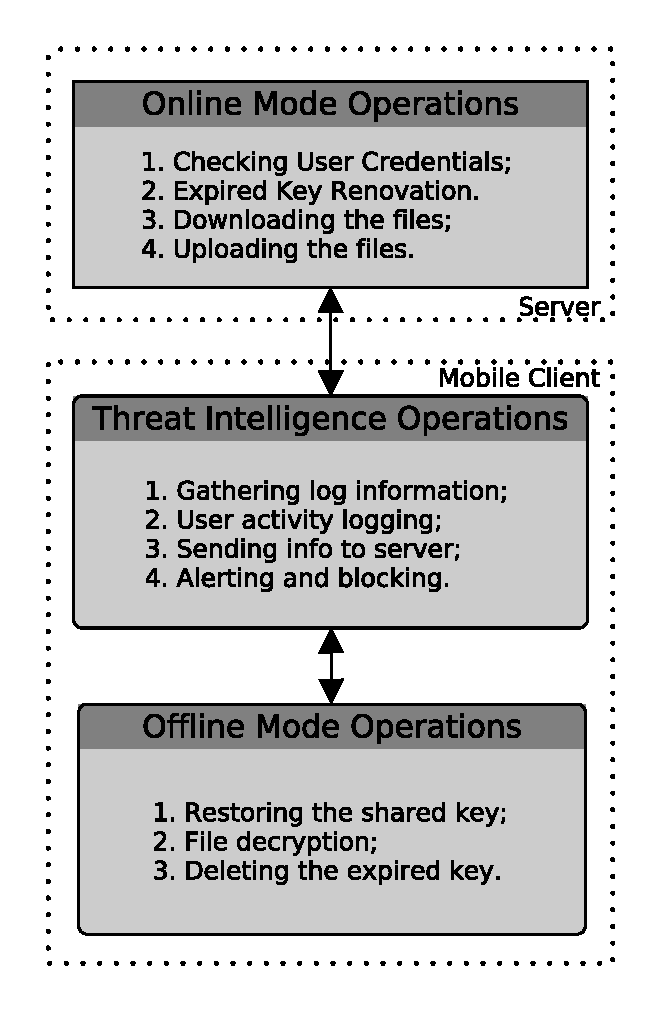
\includegraphics[width=8cm]{figures/fig01.eps}
	\caption{The core set of functions and protocols of the mobile cloud security infrastructure}
	\label{fig:3_01}
\end{figure}

Figure \ref{fig:3_01} describes the mobile client protection both in online and offline mode. In online mode, the client has the possibility to connect to the server and the security of the client is enhanced by the server-backed up mechanisms. On the other hand, in offline mode the client’s security is supported by the standalone mechanisms. Additionally, the mobile client protection is enhanced by the threat intelligence unit providing the constant monitoring and analysis.

Figure \ref{fig:3_02} depicts the client-side protection mechanisms. The client should support 4 subsystems: i) encryption subsystem (\textbf{Online/Offline Cryptography}) that contains the procedures of encryption and decryption; ii) storage subsystem (\textbf{Protected Storage}) that provides the downloaded shares and key storage protection; iii) (\textbf{threat intelligence}) unit that provides the constant monitoring, and iv) the communication subsystem (\textbf{Communication with Server}). In short, all security procedures are connected to 4 groups of operations: file request and receiving; encryption and decryption; file and key storing; monitoring and analysis.

\begin{figure}[h!]
	\centering
	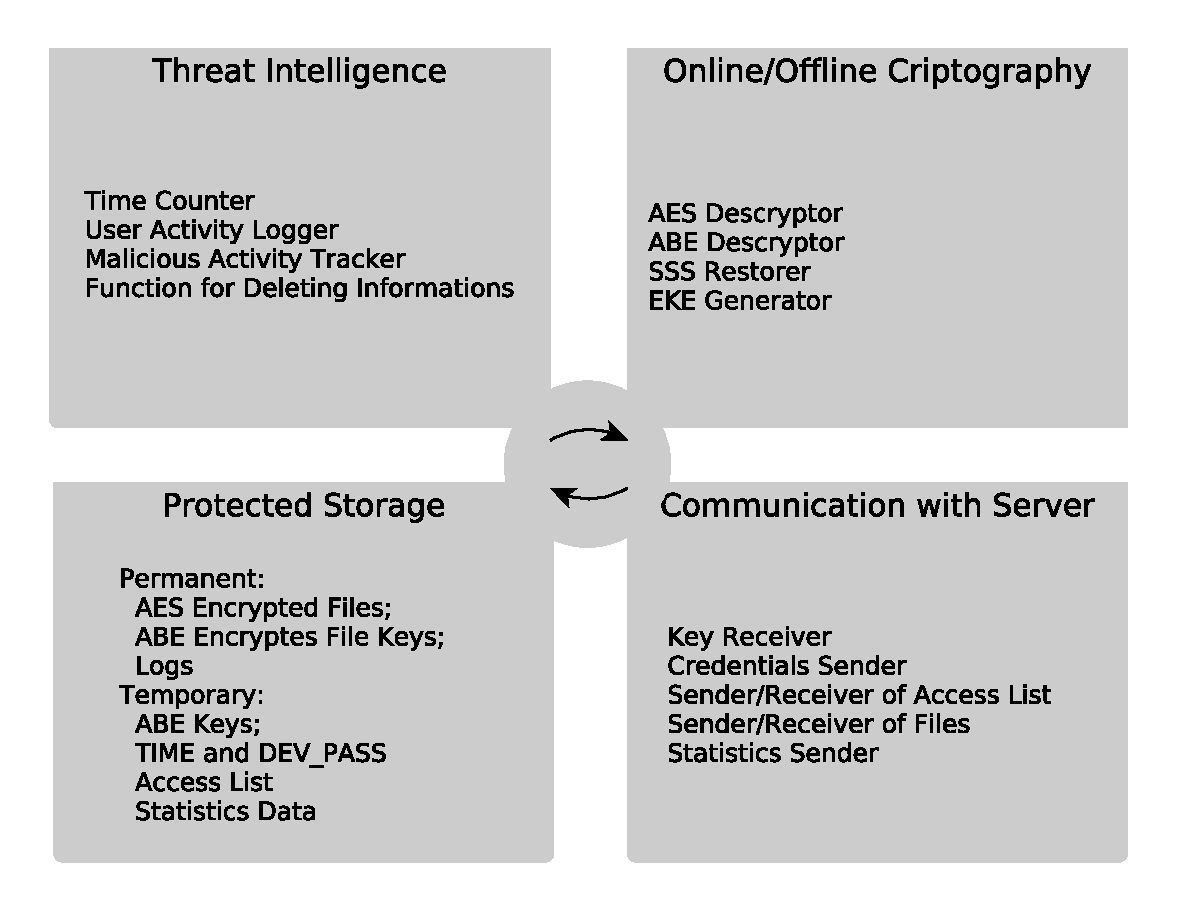
\includegraphics[width=12cm]{figures/fig02.eps}
	\caption{The Client-side Architecture}
	\label{fig:3_02}
\end{figure}

This architecture consists of the modules of cryptographic functions, threat intelligence infrastructure, communication with server and storage. However, this work focus on the threat intelligence infrastructure module for malicious behavior analysis.

The threat intelligence infrastructure takes into account simple actors such as the time counter for the key expiry period, the counter of unsuccessful tries in order to protect from brute force attacks, and MOS-inspired statistics analyzer. Functions such as alerting and deleting the expired key belong to this module as well. These functions are described in Subsection \ref{sec:3_mos}.


\section{The proposed solution for offline mobile security}
\label{sec:3_offline_mode}

This section proposes an approach for the mobile client protection in which the security is supported in offline modes. Currently and to the best of our knowledge, the systems of mobile client protection follow a model where the protected client can operate only when it is connected to the cloud, which is not always convenient for the end-user. The basic principles of the mobile client protection herein proposed are: 

\begin{enumerate}
	\item Optimized communication with the cloud when the mobile client does not need to be constantly connected to the server due to the resource constraint and necessity to secure this communication;
	\item Optimized combination of the security mechanisms so that the mobile client does not need to perform complex computation like encryption and key generation due to its resource constraint;
	\item Behavioral analysis of user's operations on mobile client, which can indicate anomalous or automated activities performed by attackers.
\end{enumerate}

The most important security issues in the proposed model arise when the client goes to the offline mode and the user is still allowed to get the access to the protected SME documents. In this case, the server can neither monitor the user activity nor provide the protection methods. The security should be performed at the mobile client. Additionally, the maximum protection should be provided at the minimum resource cost. 

In the online mode the mobile client uses the secure communication with the server in order to verify the validity of user’s credentials. On the contrary, the offline protection model should be approached independently.

\begin{figure}[h!]
	\centering
	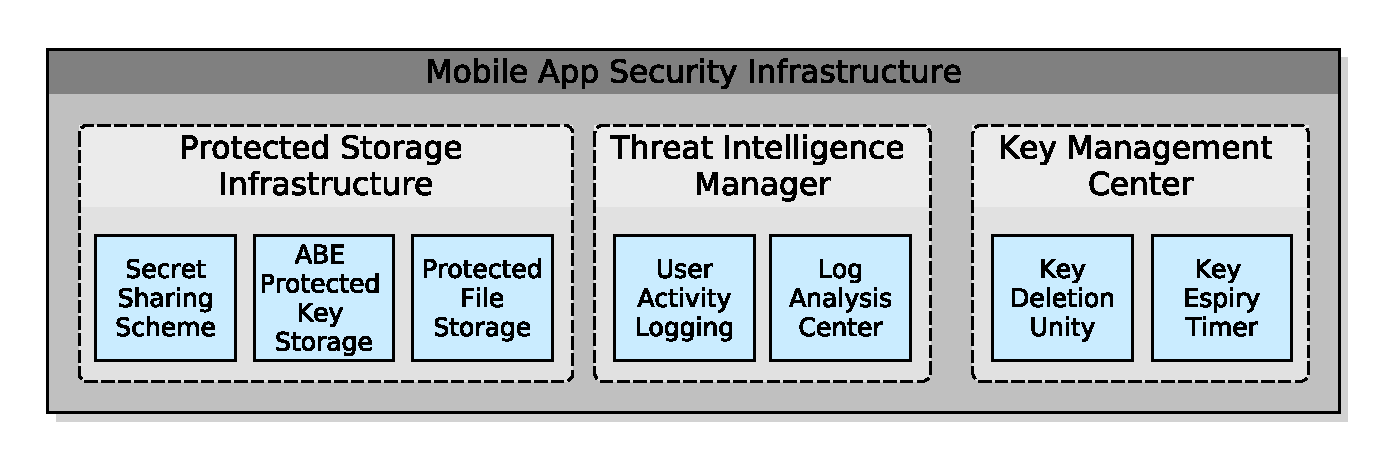
\includegraphics[width=15cm]{figures/fig03.eps}
	\caption{Proposed Architecture for Offline Mobile Security}
	\label{fig:3_03}
\end{figure}

The Figure \ref{fig:3_03} describes the proposed architecture for offline mobile security, showing the modules responsible for securing the mobile client, which includes:

\begin{enumerate}
	\item \textbf{Protected Storage}: the storage is protected with the shared user key and contains the ABE keys giving access to the file keys which allow decrypting the stored files.
	\item \textbf{Threat Intelligence Manager (TIM)}: most attacks incur into significant variation on the legitimate behavior of information systems, or they adopt well-known patterns that can be easily detected by monitoring the system in the case of the offline mode. Signal processing techniques have been successfully applied to anomaly detection \cite{lu2009network, huang2009signal} and have become a solution to a problem of improving detection accuracy, adaptability and computational cost for application on resource-constrained scenarios. Therefore, signal processing can be applied in offline mobile client security, for evaluating anomalies on user's behavior, according to the scenarios in Section \ref{sec:3_results}. Moreover, Model Order Selection (MOS), which is an effective signal processing technique to separate noise components from the principal components, can be applied into anomaly and attack detection \cite{tenorio2013greatest}, to identify and separate malicious behaviors from the legitimate ones. The TIM is an internal module of the mobile client that implements offline anomaly detection through signal processing techniques.
	\item \textbf{Key Management Center}: it includes the functions for maintaining the key expiry period and deleting the expired keys. 
\end{enumerate}


\subsection{Offline Behavioral Analysis}
\label{sec:3_offline_behavioral_analysis}

In the proposed client security architecture, the Threat Intelligence Manager (TIM) is responsible for receiving logged user operations, perform feature extraction, data modeling and malicious behavior analysis in order to identify possible threats, in offline mode. Figure \ref{fig:3_06} depicts the TIM for offline behavioral analysis. 

\begin{figure}[h!]
	\centering
	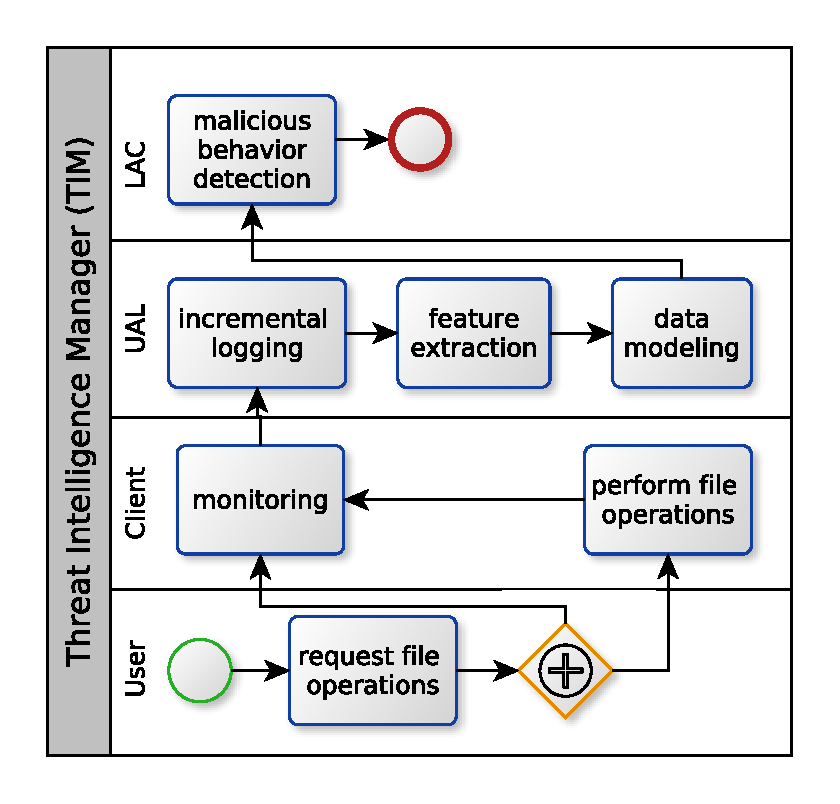
\includegraphics[width=10cm]{figures/fig06.eps}
	\caption{The Threat Intelligence Manager Workflow}
	\label{fig:3_06}
\end{figure}

As depicted in Figure \ref{fig:3_06}, users request operations are logged so that the main features can be monitored in the mobile client. The user behavior, trying or effectively executing operations, shall be incrementally captured and logged, making possible to monitor the main features that can reveal malicious behaviors, as well as to identify unexpected behaviors that can reveal possible threats. Therefore, the user operations are monitored by the client app, which sends the information to the User Activity Logging (UAL). 

The UAL is responsible for the incremental logging of activities of the mobile client, feature extraction and data modeling for malicious behavior detection, through the Log Analysis Center (LAC). As an internal module of the mobile client, the UAL implements monitors of selected events of the application, such as a login attempt or a file decryption, and logs the desired information for further analysis. The logged information shall be decomposed into selected features and modeled as matrices, composed of the number of occurrences of the selected features by its location and by time. The resultant data is submitted to the LAC, for anomaly detection.

The LAC performs the behavioral analysis through eigenvalue analysis and MOS schemes, which identify anomalies on sparse, subtle or abrupt number of user operations. The malicious behavior detection is detail described in \ref{sec:3_mos}.

\section{MOS for Threat Intelligence}
\label{sec:3_mos}
In the context of anomaly-based schemes for attack detection, the proposed behavioral analysis approach applies signal processing techniques, such as Principal Component Analysis and Model Order Selection schemes \cite{tenorio2013greatest}, for automatic detection of attacks or malicious behaviors. 

Model Order Selection is an effective signal processing technique for several applications, allowing separating the only noise components from the principal components applying a rank reduction of the data. 

Applying MOS to the analysis of user operations can be effective in order to reveal the occurrence of malicious behavior during an offline session. MOS for threat intelligence requires that the target features, which can be user operations, should be modeled as a matrix composed by the number of occurrences by location and time, and grouped into $Q$ time frames. Therefore, the framework considers the time variations of the matrix $\mathbf{X}^{(q)} \in \mathbb{R}^{M\times{N}}$, with $q = 1, \ldots, Q$, in order to detect the occurrence of malicious behaviors. For example, one element of $\mathbf{X}^{(q)}$ can represent the number of file readings on folder $m$ during the minute $n$, from file operations logged by the mobile client.

The MOS schemes can rely on sample covariance of zero mean variables (called as \textbf{zero mean covariance} for the sake of simplicity) and sample covariance of zero mean and unitary standard deviation (called as \textbf{zero mean and standardized covariance} for the sake of simplicity) variables, where the former is useful to identify abnormalities caused by large amounts of operations during a period, while the latter is applied to identify anomalies on sparse or subtle number of file operations.

Classical approaches to model order selection require the computation of the sample covariance matrix $\mathbf{\hat{R}}_{yy}^{(q)}$ and of its eigenvalues, obtained from the measurement matrix $\mathbf{X}$ of the zero mean samples given by

\begin{equation}\label{eq:3_eq03}
	\mathbf{y}_{m}^{(q)} = \mathbf{x}_{m}^{(q)} - \bar{\mathbf{x}}_{m}^{(q)}.
\end{equation}

The set of obtained vectors $\mathbf{y}_{m}^{(q)}$ composes the zero mean matrix $\mathbf{Y}^{(q)}$, then the zero mean covariance matrix $\mathbf{\hat{R}}_{yy}^{(q)}$ can be estimated as follows

\begin{equation}\label{eq:3_eq04}
	\mathbf{\hat{R}}_{yy}^{(q)} = \frac{1}{N}\mathbf{Y}^{(q)}\mathbf{Y}^{(q)^{\rm T}},
\end{equation}
where $\mathbf{\hat{R}}_{yy}^{(q)}$ means the estimation of the sample covariance matrix from the measured zero mean matrix $\mathbf{Y}^{(q)}$ over $N$ minutes of the time frame $q$. 

For MOS based on sample covariance of zero mean and unitary standard deviation, in order to identify anomalies with sparse or subtle behavior, it is required, for each variable, to make the standard deviation unitary as follows

\begin{equation}\label{eq:3_eq05}
	\mathbf{z}_{m}^{(q)} = \frac{\mathbf{x}_{m}^{(q)} - \bar{\mathbf{x}}_{m}^{(q)}}{\mathbf{\sigma}_{m}^{(q)}}.
\end{equation}

The set of vectors $\mathbf{z}_{m}^{(q)}$ composes the matrix $\mathbf{Z}^{(q)}$, then the zero mean and standardized covariance matrix $\mathbf{\hat{R}}_{zz}^{(q)}$ can be calculated via 

\begin{equation}\label{eq:3_eq06}
	\mathbf{\hat{R}}_{zz}^{(q)} = \frac{1}{N}\mathbf{Z}^{(q)}\mathbf{Z}^{(q)^{\rm T}}.
\end{equation}

Once the $\mathbf{\hat{R}}_{yy}$ or $\mathbf{\hat{R}}_{zz}$ have been obtained for MOS in order to anomaly detection, for the sake of simplicity, we refer to $\mathbf{\hat{R}}_{yy}$ or $\mathbf{\hat{R}}_{zz}$ as a matrix $\mathbf{C}$. Therefore, the next step of the algorithm is the eigenvalue decomposition (EVD), calculated according to $\mathbf{C}^{(q)} = \mathbf{V}^{(q)}\mathbf{\lambda}^{(q)}\mathbf{V}^{(q)^{\rm T}}$, in order to obtain the vector of eigenvalues $\textbf{e}$, as following:

\begin{equation}\label{eq:3_eq07}
	\mathbf{e}^{(q)} = \rm diag(\mathbf{\lambda}^{(q)}),
\end{equation}

The eigenvalues should be sorted in descending order, as defined by $\lambda_{1}^{(q)} > \lambda_{2}^{(q)} > \lambda_{3}^{(q)} > \cdots > \lambda_{m}^{(q)}$, to make possible the selection of the first eigenvalue in the obtained sequence, represented by $\lambda_{1}^{(q)}$, which is the largest eigenvalue of the data evaluated for attack detection.

The process of obtaining the $\mathbf{X}^{(q)} \in \mathbb{R}^{M\times{N}}$ and the matrix $\mathbf{C}^{(q)}$, finding the largest eigenvalue for each $q$-th time frame, should be repeated until $q = Q$, in order to obtain the largest eigenvalue of all time frames, as presented by 

\begin{equation}\label{eq:3_eq08}
	\mathbf{E} =
	\begin{bmatrix}
		\lambda_1^{(1)} & \lambda_1^{(2)} & \lambda_1^{(3)} & \cdots & \lambda_1^{(Q)} \\
		\lambda_2^{(1)} & \lambda_2^{(2)} & \lambda_2^{(3)} & \cdots & \lambda_2^{(Q)} \\
		\lambda_3^{(1)} & \lambda_3^{(2)} & \lambda_3^{(3)} & \cdots & \lambda_3^{(Q)} \\
		\vdots & \vdots & \ddots & \vdots  \\
		\lambda_m^{(1)} & \lambda_m^{(2)} & \lambda_m^{(3)} & \cdots & \lambda_m^{(Q)} \\
	\end{bmatrix}.
\end{equation}

Since $\lambda_1^{(q)} > \lambda_2^{(q)} > \lambda_3^{(q)} > \cdots > \lambda_{m-1}^{(q)} > \lambda_m^{(q)}$, then the first line of the matrix $\mathbf{E}$ contains the largest eigenvalues of each $q$-th time frame, which is the expected input for MOS schemes and can be expressed as 

\begin{equation}\label{eq:3_eq09}
	\boldsymbol{e}_{\rm max} = \boldsymbol{E}\{:,1\} = [ \lambda_1^{(1)}, \lambda_1^{(2)} \cdots \lambda_1^{(Q)}]
\end{equation}

Once obtained the largest eigenvalues of each $q$-th time frame, it is possible to apply a selected MOS scheme to estimate the model order $\hat{d}$, which is the estimated number of time frames with malicious behavior. Therefore, $\boldsymbol{e}_{\rm max}$ is used as input parameter for MOS schemes, according to the equation

\begin{equation}\label{eq:3_eq10}
	\hat{d} = \textrm{MOS}(\boldsymbol{e}_{\rm max})
\end{equation}

Note that some MOS schemes may also require the amount of time that compose a time frame, such as $\hat{d} = \textrm{MOS}(\boldsymbol{e}_{\rm max}, M)$. For more information about MOS schemes, interested readers are referred to Appendix \ref{apx:a_mos} and to \cite{da2009comparison}.


\section{Results and analysis}
\label{sec:3_results}

This section provides the detailed analysis of the results from the proposed approach regarding security and performance analysis.

\subsection{Security analysis}
\label{sec:3_sec_analysis}
The security analysis of the proposed model was performed from the user behavioral analysis. Two common attack scenarios were analyzed. First, the malicious outsider trying to infect or steal the important files. Second, the malicious expired user trying to steal the important files. 

\subsubsection{Common threat scenarios}
\label{sec:3_common}
This section provides the detailed description of the common scenarios in which the log and behavioral analysis is provided. The behavioral analysis can help to keep the user or administrator informed of the threat and take actions, as well as it can be useful in order to implement threat preventions or reactive actions to avoid threat propagation.

\begin{thm}
	An attacker uses a valid password to perform operations on a bulk of files.
\end{thm}

The session time defines the period when operations can be performed until the next session renewing. During this period, it is still necessary to identify attacks and malicious behavior on file operations, in order to avoid fast attacks to perform unauthorized access to information or data modification. Some attacks present behavioral patterns based on abrupt number of operations, such as the ransomware attack, which is a growing attack \cite{McAfee2015} that blocks the access to valuable resources and requires a payment in order to unblock the content. The access to the resources can be blocked by the attacker through some techniques, when the content is encrypted by the attacker, the ransomware attack can be called cryptoransomware or cryptolocker \cite{kaspersky2014}.

MOS schemes based on zero mean covariance analysis are effective to reveal abrupt changing of behaviors over time \cite{tenorio2013greatest}, making possible to identify intense malicious behaviors on offline mode of mobile clients, such in case of ransomware attack or bulk access to sensitive data.

The large number of operations over time is a well-known pattern of some attacks, due to the efforts on security measures to make the attacks infeasible over time. In this context, the operations can also be evaluated in contrast to the estimated required time for operations done by legitimate behaviors, such as the evaluation of the mean time between operations, highlighting the occurrence of infeasible behaviors in comparison to legitimate user activities.

Sparse or subtle file operations, with low number of operations distributed over different files or directories, during short period of time can indicate anomalies in contrast to the required time for legitimate directory navigation. MOS and zero mean and standardized covariance analysis can be suitable if applied to evaluate the time and location of operations, in order to identify unreachable navigation, if compared to legitimate navigation

The MOS based on zero mean covariance analysis indicates abnormalities caused by large amounts of operations during a period. Subsequently, the eigenvalue analysis highlights massive or concentrated operations over time or folder location, which is evaluated by MOS schemes in order to identify the number of malicious behaviors during the evaluated time.

This threat scenario, where an attacker uses a valid password and session to perform operations on a bulk of files, can have its steps described as:

\begin{enumerate}[label=(\alph*)]
	\item The hacker has access to the mobile client and is able to perform operations;
	\item The session time is valid;
	\item The hacker tries to perform legitimate operations, such as file decryption, encryption, reading, writing or directory navigations;
	\item The mobile client incrementally append each operation attempt time into the logging;
	\item The MOS module evaluates the logging of legitimate operations, applying zero mean and standardized covariance analysis to identify anomalies on sparse or subtle number of file operations, highlighting the occurrence of infeasible behaviors in comparison to legitimate user activities;
	\item The MOS module evaluates the logging of legitimate operations, applying zero mean covariance analysis to identify abnormalities caused by massive operations during the session time.
\end{enumerate}

\begin{thm}
	Usage of expired password to perform unauthorized operations.
\end{thm}

In the offline mode, the session time is used to restrict the operations during a specified period, although it is possible to manipulate the current time in mobile device, to emulate a period in which the session was valid. The log analysis by MOS can deal with this kind of threat, through the incremental logging of the time when each operation was performed, followed by the behavioral evaluation of operations over time. 

The incremental logging assumes that new logged operations shall have equal or bigger time than the last logged operation, the violation of this rule means that the system is out of sync and indicates a malicious behavior. Additionally, a large amount or sparse operation performed at the same time, or during a short period, can indicate the use of backtrack techniques to maintain a valid session during necessary time to perform an attack. Massive, subtle or sparse malicious operation performed during a valid session time can be identified by MOS schemes based on covariance analysis.

Applying MOS to the analysis of the time between user operations can be effective in order to reveal the occurrence of malicious behavior during an offline session. The MOS based on zero mean and standardized covariance analysis identifies anomalies on sparse or subtle variation in the number of file operations, since the eigenvalue analysis highlights the unexpected number of sparse (such as file operations on diverse folders) or subtle operations. Consequently, the result of the eigenvalue analysis is applied to MOS schemes, in order to identify the occurrence of malicious behaviors during the valid session.

The MOS based on zero mean covariance analysis indicates abnormalities caused by large amounts of operations during a period. The eigenvalue analysis based on the zero mean covariance matrix highlights massive or concentrated operations over time or location, which is evaluated by MOS schemes in order to identify the number of malicious behaviors during the evaluated time.

This threat scenario, where the attacker uses expired password to perform unauthorized operations, can have its steps described as:

\begin{enumerate}[label=(\alph*)]
	\item The hacker steals the operating system;
	\item The hacker modifies the time of the operating system to a period when the session was valid;
	\item The hacker has access to the mobile client and is able to perform operations;
	\item The hacker tries to perform legitimate operations, such as file decryption, encryption, reading, writing or directory navigations;
	\item The mobile client incrementally append each operation attempt time into the logging;
	\item The mobile client verifies if one logged time is older than the last operation time. If it is true, the MOS module classifies the evaluated operation as malicious;
	\item The MOS module evaluates the logging of legitimate operations, applying zero mean and standardized covariance analysis to identify anomalies on sparse or subtle number of file operations;
	\item The MOS module evaluates the logging of legitimate operations, applying zero mean covariance analysis to identify abnormalities caused by massive operations during the session time;
\end{enumerate}

\subsubsection{Data Modeling for Behavioral Analysis }
\label{sec:3_data}

MOS schemes are used in order to identify anomalous behavior that can indicate an attack and be used to prevent or avoid attack propagation. Therefore, it is necessary to analyze the data that can be collected from user operations on mobile client, to identify features that can be modeled and submitted to MOS schemes, according to described in Section \ref{sec:3_mos}.

The selected features shall be modeled as matrices which represents a signal superposition containing noise, legitimate and malicious behavior \cite{tenorio2013greatest}, grouped into time frames $\mathbf{X}^{(q)} \in \mathbb{R}^{M\times{N}}$, with $q = 1, 2, 3, \ldots, Q$ , where $M$ defines the decomposition of a selected feature, $N$ defines the time decomposition and represents the number of occurrences of the feature $m$ during the time $n$.

In offline mode, the user is still allowed to get access to operations that do not require communication with the server side. These operations and their selected features shall be incrementally logged by the UAL of the mobile client, in order to be analyzed by the TIM to identify malicious behaviors. 

This work proposes to evaluate the following features, which represents events of the user operating the mobile client.

\paragraph{\textbf{File Access (Time and File System Location)},}i.e. data access to selected files in offline mode, accessing the data stored on the mobile client. The file access feature can be decomposed into more detailed features, which are:

\begin{enumerate}
	\item number of file decryption;
	\item number of decrypted file reading;
	\item number of decrypted file execution. 
\end{enumerate}

Therefore, it is necessary to generate three matrices for the following malicious behaviors analysis: 

\begin{enumerate}[label=(\alph*)]
	\item massive file access, which can reveal data leakage and be identified by MOS schemes based on zero mean covariance analysis; 
	\item low file access into several folders, characterized by sparse operations that can reveal unreachable navigation performed by automated file accesses in order to avoid the massive file access characterization;
	\item Malicious sparse file accesses can be identified by MOS schemes based on zero mean and standardized covariance analysis. 
\end{enumerate}

\paragraph{\textbf{File Update (Time and File System Location)},}i.e. writing operations into selected files in offline mode, writing the data stored on the mobile client. The update feature can be decomposed into:

\begin{enumerate}
	\item number of file encryption;
	\item number of decrypted file writing.
\end{enumerate}

Therefore, it is necessary to generate two matrices for malicious behaviors analysis, such as: 

\begin{enumerate}[label=(\alph*)]
	\item massive file update, which can reveal ransomware or similar attacks and be identified by MOS schemes based on zero mean covariance analysis; 
	\item low number of file update into several folders, characterized by sparse operations that can reveal unreachable navigation performed by automated file accesses in order to avoid the massive file access characterization. Malicious sparse file accesses can be identified by MOS schemes based on zero mean and standardized covariance analysis.
\end{enumerate}

\paragraph{\textbf{File Download (Start Time, End Time and File System Location)},}i.e. download requests in online mode, evaluated by the mobile client. The file download feature shall be modeled as the matrix of number downloads by file location over time, in order to perform malicious behaviors analysis, such as:

\begin{enumerate}
	\item massive data leakage or similar attacks, which can be identified by MOS schemes based on zero mean covariance analysis;
	\item low number of file download from several folders, characterized by sparse operations, which can reveal unreachable navigation performed by automated file download in order to avoid the massive file download characterization. Malicious sparse file download can be identified by MOS schemes based on zero mean and standardized covariance analysis.
\end{enumerate}

\paragraph{\textbf{File Upload (Start Time, End Time and File System Location)},}i.e. upload requests in online mode, evaluated by the mobile client. The file upload feature can reveal attempts of ransomware or similar attacks and be identified by MOS schemes based on covariance analysis. Therefore, it is necessary model the matrix of number uploads by file location over time, in order to perform malicious behaviors analysis, such as:

\begin{enumerate}
	\item massive file upload, similar to ransomware attack, which can be identified by MOS schemes based on zero mean covariance analysis; 
	\item low number of file upload to several folders, characterized by sparse operations, which can reveal unreachable navigation performed by automated file upload in order to avoid the massive file upload characterization. Malicious sparse file upload can be identified by MOS schemes based on zero mean and standardized covariance analysis.
\end{enumerate}

\subsection{Performance analysis}
\label{sec:3_complex}


The proposed concept of mobile client security has been implemented in the Storgrid protected cloud environment \cite{storgrid2016}. Therefore, the approach is correlated with the practical usability requirements: the corporate user continues to use the mobile storage app in offline and does not need to reload the files every time the key is renewed. This methodology can be used in other mobile clients. The common advantage is that the mobile client performs the operations both in the offline and online mode and uses the key expiry to protect the privacy of the corporate data. 

The log analysis of the Log Analysis Center (LAC) has been implemented and evaluated for offline anomaly detection in mobile clients, making it possible to apply anomaly detection techniques in a lightweight fashion, considering low processing requirements for deal with the resource constraints of mobile clients. The evaluation considered the required processing time for anomaly detection from log analysis, measuring the data modeling time through the UAL, the eigenvalue decomposition time and the required time for the EDC MOS scheme execution, which is the scheme that requires less processing capacity and provides more anomaly identification accuracy \cite{da2009comparison,tenorio2013greatest}. 

The experiments were performed in two mobile devices, Galaxy GT-I9300 and Galaxy Tab SM-T800, with variations of log size and window size. The Galaxy GT-I9300 has Quad-core 1.4 GHz Cortex-A9 processor and 1 GB RAM, while the Galaxy Tab SM-T800 has its processing capacity composed by Quad-core 1.9 GHz Cortex-A15 and quad-core 1.3 GHz Cortex-A7, and 3 GB RAM.

Table \ref{tab:3_04} presents the data modeling time and the processing time of eigenvalues decomposition calculations to be applied to anomaly detection from user operation logs of Storgrid mobile client. 

\begin{table*}
	\caption{Data Modeling and Eigenvalue Decomposition Time}
	\scriptsize
	\label{tab:3_04}
	\centering
	\begin{tabular}{|l|l|l|l|l|l|l|l|}
		\hline \rowcolor{Gray} Device	& \begin{tabular}[x]{@{}l@{}}Log Size\\(MB)\end{tabular}	& \begin{tabular}[x]{@{}l@{}}Window\\(min)\end{tabular}	& \begin{tabular}[x]{@{}l@{}}Modeling\\(ms)\end{tabular}	& \begin{tabular}[x]{@{}l@{}}Avg. Eig.\\(ms)\end{tabular}	& \begin{tabular}[x]{@{}l@{}}Std. Eig.\\(ms)\end{tabular}	& \begin{tabular}[x]{@{}l@{}}Eig. Min.\\(ms)\end{tabular}	& \begin{tabular}[x]{@{}l@{}}Eig. Max.\\(ms)\end{tabular}	\\ \hline
		Galaxy GT-I9300	& 6	& 60	& 107	& 209.52	& 18.58	& 183	& 276	\\ \hline
		Galaxy GT-I9300	& 6	& 40	& 115	& 227.26	& 18.13	& 191	& 289	\\ \hline
		Galaxy GT-I9300	& 6	& 20	& 89	& 268.14	& 21.94	& 229	& 315	\\ \hline
		Galaxy GT-I9300	& 6	& 10	& 90	& 347.42	& 24.11	& 304	& 421	\\ \hline
		Galaxy GT-I9300	& 4.1	& 60	& 20	& 60.90	& 15.19	& 37	& 106	\\ \hline
		Galaxy GT-I9300	& 4.1	& 40	& 20	& 68.72	& 15.71	& 43	& 114	\\ \hline
		Galaxy GT-I9300	& 4.1	& 20	& 34	& 89.04	& 16.78	& 54	& 133	\\ \hline
		Galaxy GT-I9300	& 4.1	& 10	& 21	& 117.24	& 14.36	& 96	& 171	\\ \hline
		Galaxy GT-I9300	& 1.4	& 60	& 10	& 159.82	& 15.82	& 125	& 197	\\ \hline
		Galaxy GT-I9300	& 1.4	& 40	& 10	& 168.06	& 15.90	& 139	& 220	\\ \hline
		Galaxy GT-I9300	& 1.4	& 20	& 11	& 204.4	& 20.46	& 176	& 269	\\ \hline
		Galaxy GT-I9300	& 1.4	& 10	& 13	& 259.00	& 21.34	& 220	& 315	\\ \hline
		Galaxy Tab SM-T800	& 6	& 60	& 7	& 59.30	& 6.55	& 54	& 74	\\ \hline
		Galaxy Tab SM-T800	& 6	& 40	& 8	& 62.56	& 7.05	& 56	& 80	\\ \hline
		Galaxy Tab SM-T800	& 6	& 20	& 10	& 73.28	& 8.59	& 65	& 95	\\ \hline
		Galaxy Tab SM-T800	& 6	& 10	& 8	& 93.48	& 9.13	& 83	& 130	\\ \hline
		Galaxy Tab SM-T800	& 4.1	& 60	& 11	& 18.64	& 4.51	& 16	& 38	\\ \hline
		Galaxy Tab SM-T800	& 4.1	& 40	& 11	& 19.64	& 5.12	& 17	& 38	\\ \hline
		Galaxy Tab SM-T800	& 4.1	& 20	& 12	& 25.12	& 5.55	& 21	& 46	\\ \hline
		Galaxy Tab SM-T800	& 4.1	& 10	& 12	& 32.32	& 7.29	& 27	& 55	\\ \hline
		Galaxy Tab SM-T800	& 1.4	& 60	& 4	& 49.08	& 6.01	& 42	& 62	\\ \hline
		Galaxy Tab SM-T800	& 1.4	& 40	& 5	& 51.42	& 7.36	& 44	& 74	\\ \hline
		Galaxy Tab SM-T800	& 1.4	& 20	& 5	& 51.12	& 7.80	& 54	& 91	\\ \hline
		Galaxy Tab SM-T800	& 1.4	& 10	& 7	& 75.24	& 7.71	& 65	& 90	\\ \hline
	\end{tabular}
\end{table*}

The information presented by column are the device model, the log size in megabytes, the window size in minutes, the data modeling time in milliseconds, the average of eigenvalue decomposition time in milliseconds, the standard deviation of eigenvalue decomposition time in milliseconds, the minimum of eigenvalue decomposition time in milliseconds and the maximum of eigenvalue decomposition time in milliseconds.

The results show that the lower window size leads to the larger eigenvalue decomposition time, but the largest eigenvalue decomposition time, which was the maximum of 421 milliseconds with average of 347.42 milliseconds. This result highlights an acceptable speed even for the worst evaluated scenario, which is the case using a Galaxy GT-I9300 for processing 6MB with window size of 10 minutes.

\begin{table*}[!t]
	\caption{EDC MOS scheme processing time for anomaly detection}
	\footnotesize
	\label{tab:3_05}
	\centering
	\begin{tabular}{|l|l|l|l|l|l|l|l|}
		\hline \rowcolor{Gray} Device	& \begin{tabular}[x]{@{}l@{}}Log Size\\(MB)\end{tabular}	& \begin{tabular}[x]{@{}l@{}}Window\\(min)\end{tabular}	& \begin{tabular}[x]{@{}l@{}}Avg. EDC.\\(ms)\end{tabular}	& \begin{tabular}[x]{@{}l@{}}Std. EDC.\\(ms)\end{tabular}	& \begin{tabular}[x]{@{}l@{}}Min. EDC.\\(ms)\end{tabular}	& \begin{tabular}[x]{@{}l@{}}Max. EDC.\\(ms)\end{tabular}	\\ \hline
		Galaxy GT-I9300	& 6	& 60	& 5.27	& 4.04	& 3	& 20	\\ \hline
		Galaxy GT-I9300	& 6	& 40	& 10.78	& 6.37	& 6	& 34	\\ \hline
		Galaxy GT-I9300	& 6	& 20	& 32.62	& 12.44	& 21	& 88	\\ \hline
		Galaxy GT-I9300	& 6	& 10	& 115.08	& 17.45	& 88	& 158	\\ \hline
		Galaxy GT-I9300	& 4.1	& 60	& 5.68	& 4.18	& 3	& 23	\\ \hline
		Galaxy GT-I9300	& 4.1	& 40	& 10.76	& 5.31	& 7	& 27	\\ \hline
		Galaxy GT-I9300	& 4.1	& 20	& 37.58	& 10.30	& 23	& 61	\\ \hline
		Galaxy GT-I9300	& 4.1	& 10	& 125.98	& 18.56	& 101	& 191	\\ \hline
		Galaxy GT-I9300	& 1.4	& 60	& 4.92	& 3.49	& 3	& 17	\\ \hline
		Galaxy GT-I9300	& 1.4	& 40	& 9.00	& 4.23	& 6	& 25	\\ \hline
		Galaxy GT-I9300	& 1.4	& 20	& 30.14	& 9.21	& 19	& 62	\\ \hline
		Galaxy GT-I9300	& 1.4	& 10	& 100.62	& 15.83	& 69	& 163	\\ \hline
		Galaxy Tab SM-T800	& 6	& 60	& 1.84	& 0.65	& 1	& 3	\\ \hline
		Galaxy Tab SM-T800	& 6	& 40	& 3.26	& 1.24	& 2	& 7	\\ \hline
		Galaxy Tab SM-T800	& 6	& 20	& 10.90	& 2.40	& 9	& 21	\\ \hline
		Galaxy Tab SM-T800	& 6	& 10	& 41.86	& 7.33	& 34	& 60	\\ \hline
		Galaxy Tab SM-T800	& 4.1	& 60	& 1.85	& 0.60	& 1	& 3	\\ \hline
		Galaxy Tab SM-T800	& 4.1	& 40	& 3.62	& 1.10	& 2	& 8	\\ \hline
		Galaxy Tab SM-T800	& 4.1	& 20	& 12.04	& 2.79	& 9	& 22	\\ \hline
		Galaxy Tab SM-T800	& 4.1	& 10	& 40.16	& 6.48	& 35	& 60	\\ \hline
		Galaxy Tab SM-T800	& 1.4	& 60	& 1.98	& 0.89	& 1	& 6	\\ \hline
		Galaxy Tab SM-T800	& 1.4	& 40	& 3.30	& 1.16	& 2	& 7	\\ \hline
		Galaxy Tab SM-T800	& 1.4	& 20	& 10.48	& 2.90	& 8	& 21	\\ \hline
		Galaxy Tab SM-T800	& 1.4	& 10	& 34.52	& 4.08	& 30	& 45	\\ \hline
	\end{tabular}
\end{table*}

Table \ref{tab:3_05} presents the processing time of EDC MOS calculations applied to anomaly detection from user operation logs of Storgrid mobile client. Table \ref{tab:3_05} respectively presents the device model, the log size in megabytes, the window size in minutes, the average of EDC calculation time in milliseconds, the standard deviation of EDC calculation time in milliseconds, the minimum of EDC calculation time in milliseconds and the maximum of EDC calculation time in milliseconds.

It is possible to observe that the processing time increases with the window size decreasing, similar to the results for eigenvalue decomposition time. The longest processing time measured is lower than 200 milliseconds, even considering window size of 10 minutes or processing 6 MB of user operation log. This result represents an acceptable processing time for anomaly detection in mobile clients.

\section{Conclusion and future work}
\label{sec:3_conclusion}

An important security issue faced by corporations that use cloud-based systems is how to provide security mechanisms to support offline corporate mobile clients. Once a mobile client releases the connection with the corporate cloud, no security measure implemented in the cloud infrastructure assures the protection of sensitive data stored in the mobile device. Aware of this problem and its importance, this work presented a proposal to address the offline mobile security problem combining a different cryptographic methods. Moreover, this proposed approach also prevents malicious user behavior by applying a MOS-based analytic method. 

As prove of concept, a fully working mobile application was developed to test the proposed security solution and acquired results provide evidence that besides achieving the desired security features, the solution also has positive results in terms of performance. This fact is due to the usage of lightweight operations and the optimized combination of the selected security methods. The proposed approach is a practical application to be used in the corporate mobile environment. It is implemented as a fully working mobile client and can be used for any type of enterprise. Also, part of concept is seed for new security solutions for big data apps. 

Future works in the area can further explore enhancements in the analytics methods as well as to extended the approach to be evaluate multidimensional data through tensor-based analysis.
\chapter{Tensor-based Discriminative Sensing for Fraud Detection}
\label{ch:4_tensor_dl}

\begin{quotation}[]{Paulo Freire}
No one knows it all. No one is ignorant of everything. We all know something. We are all ignorant of something.
\end{quotation}

% \section{Introduction}
% Compressed Sensing | Dictionary Learning | Multidimensional data | Tensor DL and Separable dictionaries

Compressed Sensing (CS) aims to obtain the most relevant information of a dataset, what makes it useful for compression, signal reconstruction, image processing and classification, such as in sparse representation classification (SRC) problems. 

Dictionary learning is related to CS but seeks to obtain compact and meaningful signal representations, known as dictionary, from learning algorithms or models. DL is a signal processing technique for sparse representation of signals as basis vectors, learning the representations from training data, as dictionaries. DL is based on the principle that some observations can be described by a sparse subset of atoms taken from a redundant dictionary, which represents the causes of some observations of the world. The sparse representation in terms of such dictionaries has attracted increased interest for compressive sensing and for solving problems such as denoising, compression, image processing, data decomposition, feature extraction and classification, when the learning includes a class separability criteria in the objective function \cite{tosic2011dictionary, zhang2010discriminative, zhu2016coupled,ravishankar2011mr}. 

There are two major approaches for DL. First is the analytic approach, in which Discrete Cosine Transform basis, wavelets, curvelets and other nonadaptive functions are used as atoms to construct the dictionaries. Second is the learning-based approaches, such as the unsupervised learning for dictionary construction [9] and the online dictionary learning [11], [10], which use machine learning methods to construct the dictionary. 

In the analytic approach, some pre-defined functions are used to construct the dictionary. Curvelets [24], which tracks the shape of the discontinuity set, offers efficient and near-optimal representation of smooth objects. Shearlets [25], which is obtained from dilations, action of translations and shear transformations, has nice geometric properties and mathematical properties for image representation. Bandelets [26], which specifies the geometry as a vector field, is designed to improve the image compression and noise reduction performance. 

In the learning-based approach, machine learning methods are used to construct the dictionary from the training data. The least square error is used by the method of the optimal directions (MOD) [27] to update the dictionary iteratively. While analytic dictionaries permit to capture the global structure of a signal and allow a fast implementation, learned dictionaries often perform better in applications as they are more adapted to the considered class of signals.

In some applications, the data and its dictionary are multidimensional, e.g., when estimating jointly behavior of users in social networks. Computing tensor decompositions of multi-way datasets is particularly useful to extract hidden patterns and structure in multidimensional data analytics problems \cite{kolda2009tensor}. Tensor-based algorithms for DL can improve the performance for cases of multidimensional and separable data, regarding the dictionary identification rating, the required number of training samples and iterations for the optimization problem \cite{roemer2014tensor}. 

In imagery, the numerical burden for (i) learning a dictionary and for (ii) employing the dictionary for reconstruction tasks only allows to deal with relatively small image patches that only capture local image information. Separable dictionaries aims at overcoming these drawbacks by allowing a separable structure on the dictionary throughout the learning process. On the one hand, this permits larger patch-sizes for the learning phase, on the other hand, the dictionary is applied efficiently in reconstruction tasks. 

Multidimensional parameter estimation and learning multidimensional separable dictionaries are growing research problems. The crucial idea about separable dictionaries is to allow the dictionary to have a separable structure, where separable means that the dictionary $\textbf{D}$ is given by the Kronecker product of two smaller dictionaries $\boldsymbol{A}^{(1)} \in \mathbb{R}^{h \times a}$ and $\boldsymbol{A}^{(2)} \in \mathbb{R}^{w \times b}$, for example. Roemer \emph{et al.} \cite{roemer2014tensor} show that the multidimensional dictionary estimation problem can be efficiently formulated in terms of tensors, and that their results outperform existing schemes by exploiting the multilinear structure of the problem.

Considering that big data problems require techniques to deal with multidimensional data in order to make sense of structure and relationship of many dimensions, and also considering that a key challenge to use sparse coding and dictionary learning for classification is how to find proper dictionaries and coefficients that highlight discriminative structure and relationships of one dataset, this work propose a tensor-based DL for fraud detection from imbalanced data, in order to apply the tensor decomposition for DL methods to highlight the discriminative sensing of a fraud detection dataset. 

This chapter is organized as follows. Section \ref{sec:4_motivation} presents one experiment and results that motivate the proposed work. In Section \ref{sec:4_relatedworks}, related works are discussed. Section \ref{sec:4_datamodel} presents the data model and the evaluated datasets. Section \ref{sec:4_proposal} describes the proposed approach for fraud detection from mobile money transactions. Section \ref{sec:2_experimentalresults} discusses the experimental validation and presents the results, and Section \ref{sec:4_conclusion} draws the conclusions and the suggestions for future work.


\section{Motivation}
\label{sec:4_motivation}

Existing DL schemes can be applied to multidimensional analysis and obtain valuable results. However, the performance of tensor-based algorithms for recovering of a known separable dictionary outperform existing schemes when dealing with growing multidimensional datasets.

Considering that DL aims to obtain meaningful dictionaries, it is possible to evaluate DL algorithms by their performance to generate dictionaries that better represent one target data. Therefore, we can compare DL algorithms regarding recovering of a known dictionary. We conduct a evaluation of tensor-based DL algorithms for recovering a known dictionary in order to analyze the gains of tensor-based approaches in comparison to well known algorithms.

\subsection{Data Model and Experiments}
\label{sec:4_motivation_datamodel}

Consider a generic sparse recovery problem of the following form

\begin{equation}\label{eq:4_eq01}
	\boldsymbol{X} = \boldsymbol{A} \cdot \boldsymbol{S} + \boldsymbol{W},
\end{equation}

where $\boldsymbol{X} \in \mathbb{C}^{M \times T}$ represents $T$ consecutive observations from $M$ features, $\boldsymbol{A} \in \mathbb{C}^{M \times N}$ is the overcomplete dictionary where $N \ll T$, $\boldsymbol{S} \in \mathbb{C}^{N \times T}$ represents the sparse coefficient matrix, $\boldsymbol{W} \in \mathbb{C}^{M \times T}$ is the additive noise, and $M < N < T$.

Consider a sparse recovery problem for a separable 2-D dictionary that we can write as

\begin{equation}\label{eq:4_eq02}
	\boldsymbol{X} = (\boldsymbol{A}^{(1)} \otimes \boldsymbol{A}^{(2)}) \cdot \boldsymbol{S} + \boldsymbol{W},
\end{equation}

where $\boldsymbol{A} = (\boldsymbol{A}^{(1)} \otimes \boldsymbol{A}^{(2)})$, $\boldsymbol{A}^{(1)} \in \mathbb{C}^{M_1 \times N_1}$, $\boldsymbol{A}^{(2)} \in \mathbb{C}^{M_2 \times N_2}$, $M = M_1 \times M_2$, and $N = N_1 \times N_2$.

In order to evaluate tensor-based DL algorithms for recovering a known dictionary, we generate two random dictionaries $\boldsymbol{A}^{(1)}$ and $\boldsymbol{A}^{(2)}$ from an i.i.d. zero mean Gaussian random process, and calculate the dictionary $\boldsymbol{A}$ through the Kronecker product, according to 

\begin{equation}\label{eq:4_eq03}
	\boldsymbol{A} = (\boldsymbol{A}^{(1)} \otimes \boldsymbol{A}^{(2)}).
\end{equation}

Therefore, $\boldsymbol{A}$ is the known dictionary that shall be used for recovery evaluation. 

Subsequently, we generate a synthetic data set $\boldsymbol{X}$ using the given dictionary $\boldsymbol{A}$, according to Equation \ref{eq:4_eq01}, where $\boldsymbol{S}$ is a random sparse coefficient matrix for what we assume that each column has $K = 5$ non-zero entries, and $\boldsymbol{W}$ is the additive white gaussian noise. Thus, we estimate the initial $\boldsymbol{\hat{A}}$ dictionary from a normalized subset of $\boldsymbol{X}$ and make the dictionary separable decomposing the approximation of $\boldsymbol{\hat{A}}$ and generating $\boldsymbol{\hat{A}}^{(1)}$ and $\boldsymbol{\hat{A}}^{(2)}$ according to \cite{van1993approximation}. Afterward, we update $\boldsymbol{\hat{A}}$ through 

\begin{equation}\label{eq:4_eq04}
	\boldsymbol{\hat{A}} = (\boldsymbol{\hat{A}}^{(1)} \otimes \boldsymbol{\hat{A}}^{(2)}),
\end{equation}

and use it for DL experiments using MOD \cite{engan1999method}, K-SVD \cite{aharon2006rm}, RLS-DLA \cite{skretting2010recursive}, T-MOD \cite{roemer2014tensor} and K-HOSVD \cite{roemer2014tensor}. Due to its low computational complexity, we employ the Orthogonal Matching Pursuit (OMP) algorithm\cite{davis1997adaptive} for the sparse recovery stage in all the dictionary learning algorithms, assuming that K is known. However, other solver for sparse recovery can be used, such as Basis Pursuit \cite{chen2001atomic}, the LASSO algorithm \cite{tibshirani1996regression} or greedy \cite{davis1997adaptive}.

The final estimated dictionaries $\boldsymbol{\hat{A}}$ recovered by each DL algorithm are compared to the known dictionary $\boldsymbol{A}$, through a measure of the distance between two dictionaries. The recovered dictionary is then compared to the known dictionary, by using the angle between a known atom and a recovered atom as a distance measure. The number of identified atoms is computed by comparing these angles to a limit of $\beta_{lim} = 8.11$ degrees, that corresponds to the case where the inner product of the two compared atoms is equal to 0.99, and where each atom has 2-norm equal to 1.

For this experiments we adopt an additive noise with $snr = 20$ and 100 iterations for dictionary learning. All experiments run 100 trials in order to obtain confident results.

This evaluation extends Roemer \emph{et al.} \cite{roemer2014tensor} including RLS-DLA for comparison, and for adding the evaluation of the degree distribution for atom identification and the evaluation of the atom identification according to the dictionary size variation. Additionally, we conduct a experimental evaluation, while Roemer \emph{et al.} \cite{roemer2014tensor} presents numerical results obtained via Monte Carlo simulations.


\subsection{Results}
\label{sec:4_motivation_results}

Figures \ref{fig:fig1} and \ref{fig:fig2} show the evaluation of tensor-based (K-HOSVD \cite{roemer2014tensor} and T-MOD \cite{roemer2014tensor}) and traditional DL algorithms (RLS-DLA, K-SVD and MOD) for dictionary reconstruction of a multidimensional and separable data. These figures show the distribution of the cumulative atom identification over the degree rates.

Figure \ref{fig:fig1} presents the results for recovering a dictionary of $M=20$ and $N=50$. We see that the RLS-DLA method performs better than other methods, although T-MOD presents the best results for identification of up to 15 atoms of 50. It is possible to observe that T-MOD and K-HOSVD are better than MOD and K-SVD, and that the tensor-based methods outperforms MOD and K-SVD significantly for this experiment. Finally, Figure \ref{fig:fig1} shows that RLS-DLA recovered almost 40 atoms in $\beta_{lim} = 8.11$ degrees, while other methods present results lower results.

\begin{figure}[!htb]
	\centering 
	\includegraphics[width=10cm]{figures/5_20_2000_1000_100.eps}
	\caption{Cumulative atom identification per degree rates. $T=2000$, $M=20$, $N=50$}
	\label{fig:fig1}
\end{figure}

Figure \ref{fig:fig2} presents the results for recovering a dictionary of $M=80$ and $N=30$. It is possible to observe that the tensor-base methods outperform MOD, RLS-DLA and K-SVD in number of identified atoms and the required degrees for identification. Note that MOD performs quite similar to RLS-DLA, while K-SVD is the worst evaluated case for this experiment. Considering the tensor-based methods, T-MOD outperforms K-HOSVD with higher atom identification over lower degrees. The experimental results verify that the tensor-based dictionary learning algorithms are able to identify more dictionary atoms when dealing with larger dictionaries and that they converge faster.

\begin{figure}[!htb]
	\centering 
	\includegraphics[width=10cm]{figures/5_20_2000_24000_100.eps}
	\caption{Cumulative atom identification per degree rates. $T=2000$, $M=80$, $N=300$}
	\label{fig:fig2}
\end{figure}

The results reveals that tensor-based algorithms can perform better for dictionary recovery problems when the dictionary size increases. Since dictionary learning and reconstruction error are usually used for sparse representation classification (SRC) problems, it is possible to suppose that tensor-based algorithms can improve results of classification problems, as well as can extract hidden patterns and structure in multidimensional data analytics problems.

Recent developments in science and technology have enabled the growth and availability of raw data to occur at an explosive rate. This has created an immense opportunity for knowledge discovery and data engineering research to play an essential role in a wide range of applications from daily civilian life to national security. However, the high availability of raw data increases the challenges related to big data analytics and to imbalanced data, which corresponds to data sets exhibiting significant imbalances of classes or rare events of some classes. The fundamental issue with the imbalanced learning problem is the ability of imbalanced data to significantly compromise the performance of most standard learning algorithms

A key challenge to use SC and DL for classification is how to find proper dictionaries and coefficients that highlight discriminative structure and relationships of one dataset. Therefore, we introduce a tensor-based DL method for fraud detection from unbalanced data. Specifically, we apply a sparse representation based classification (SRC) method through learning a tensor-based dictionary and evaluate the reconstruction error for fraud classification. 

In this chapter, we propose a tensor-based sparse representation and dictionary learning technique to analyze mobile money transactions in order to identify frauds. We propose to use tensor-based DL for learning fraudulent and legitimate data separately, and apply the learned dictionaries to reconstruct a test signal and classify it as fraud or legitimate, according to the minimum reconstruction error measured by some metrics.


\section{Related Works}
\label{sec:4_relatedworks}

% Compressed Sensing | Dictionary Learning | Classification | Tensor-Based DL

Compressed sensing (also known as compressive sensing, compressive sampling, or sparse sampling) is a signal processing technique for efficiently acquiring and reconstructing a signal, by finding solutions to undetermined linear systems. This is based on the principle that, through optimization, the sparsity of a signal can be exploited to recover it from far fewer samples than required by the Shannon-Nyquist sampling theorem. 

%There are two conditions under which recovery is possible.[1] The first one is sparsity which requires the signal to be sparse in some domain. The second one is incoherence which is applied through the isometric property which is sufficient for sparse signals.[2][3]. Around 2004, Emmanuel Candès, Terence Tao, and David Donoho proved that given knowledge about a signal's sparsity, the signal may be reconstructed with even fewer samples than the sampling theorem requires.[4][5] This idea is the basis of compressed sensing. 	https://www.wired.com/2008/03/engineers-test-highly-accurate-face-recognition/

Sparse coding is a sparse representation of one data in the form of a linear combination of basic elements. These elements are called atoms and they compose a dictionary. Dictionary learning is a representation learning method which aims at finding a sparse representation of the input data (also known as sparse coding) in the form of a linear combination of basic elements as well as those basic elements themselves. These elements are called atoms and they compose a dictionary. Atoms in the dictionary are not required to be orthogonal, and they may be an over-complete spanning set. This problem setup also allows the dimensionality of the signals being represented to be higher than the one of the signals being observed. The above two properties lead to having seemingly redundant atoms that allow multiple representations of the same signal but also provide an improvement in sparsity and flexibility of the representation.

One of the key principles of dictionary learning is that the dictionary has to be inferred from the input data. The emergence of sparse dictionary learning methods was stimulated by the fact that in signal processing one typically wants to represent the input data using as few components as possible. Before this approach the general practice was to use predefined dictionaries (such as Fourier or wavelet transforms). However, in certain cases a dictionary that is trained to fit the input data can significantly improve the sparsity, which has applications in data decomposition, compression and analysis and has been used in the fields of image denoising and classification, video and audio processing. Sparsity and overcomplete dictionaries have immense applications in image compression, image fusion and inpainting.

MOD \cite{engan1999method} is a DL algorithm that is commonly used for extensions of Least-Squares (LS) type schemes, also known as iterative least squares dictionary learning algorithm (ILS-DLA) \cite{engan2007family}. MOD defines that if we know $\boldsymbol{S}$ in equation \ref{eq:4_eq01}, $\boldsymbol{A}$ can be estimated solving a linear LS problem. Additionally, knowing $\boldsymbol{A}$ we obtain $\boldsymbol{S}$ by solving a sparse recovery problem. MOD iterates between the two steps, starting with an initial guess of $\boldsymbol{A}$, denoted as $\hat{\boldsymbol{A}}$, which can be estimated, generated by previous dictionary learning or generated analytically. Despite - simplicity, the MOD algorithm has been criticized for its slow convergence, which is due to the fact that $\boldsymbol{A}$ and $\boldsymbol{S}$ are updated separately, which may lead to a slow convergence \cite{aharon2006rm}.

K-SVD \cite{aharon2006rm} is a generalization of the K-means algorithm for dictionary learning. After the sparse approximation step, the dictionary update is performed by sequentially updating each column of $\boldsymbol{A}$ using SVD to minimize the approximation error. The update step is hence a generalized K-means algorithm since each patch can be represented by multiple atoms and with different weights. In practice, dictionaries learned with K-SVD
have shown excellent performance in image denoising. 

Most DL algorithms update the dictionary after a batch of training vectors has been processed, usually using the whole set of training vectors as one batch. The training set is used iteratively to gradually improve the dictionary. The approach in RLS-DLA \cite{skretting2010recursive} is a continuous update of the dictionary as each training vector is being processed. The algorithm is based on recursive least squares (RLS) algorithm for adaptive filtering, what makes the algorithm less dependent on the initial dictionary and it improves both convergence properties of RLS-DLA as well as the representation ability of the resulting dictionary. 

Dimensionality reduction can first be achieved by selecting a subset of functions from a large, fixed dictionary that is used for the analysis of particular signals. These functions then determine a subspace of reduced dimension, where classification can be performed by computing the nearest neighbor points among the projected data. A simple method to build such a subspace consists in modifying the sparse approximation methods such that the objective function is augmented with a discrimination term that represents the separability properties of the projection subspace. This kind of approach typically tries to maximize the variance between the active atoms from $\boldsymbol{A}$ that represent signals in different classes. The reduced subspace used for classification is finally formed by the subset of atoms in $\boldsymbol{A}$ whose corresponding coefficients in $\boldsymbol{S}$ are nonzero. The subset selection problem can be interpreted as the inference step in the dictionary learning methods when the objective function is modified to include a discriminative term \cite{tosic2011dictionary}.

An important advantage of redundant dictionaries for classification is that signal analysis can be performed with functions that are likely to match the data characteristics in different classes of signals. Similarly to data approximation problems, data analysis applications can further benefit from dictionary learning methods. The previous section describes subspace selection methods from predefined dictionaries. DL algorithms can improve the classification performance, as it leads to a better adaptation of the dictionary by enforcing sparsity in the representation of data in the different classes. The atoms in a dictionary $\boldsymbol{A}$ that is computed with dictionary learning methods generally capture the most important constitutive components of the signals. They naturally permit to classify the data into the corresponding linear subspace. However, there is no guarantee that the subspace built on a learned dictionary $\boldsymbol{A}$ is truly optimal for classification, as it targets efficient representation but not necessarily class separability \cite{tosic2011dictionary}.

Dictionary learning methods should rather be modified so that they become simultaneously reconstructive and discriminative. The addition of a discriminative term into the dictionary learning algorithms requires supervision, where labels of training data are used to ensure that the data representation is sufficiently different in each class. It can be achieved by modifying the sparse coding step in the learning algorithms, so that it optimizes an objective function that favors the sparsest representation of a given signal and simultaneously the representation that is also the most different from the one of signals in other data classes. The supervised dictionary learning problem can be cast as a mixed formulation that minimizes the average value of the sparse approximation errors over different classes and also enforces discrimination between classes \cite{tosic2011dictionary}.

The use of one learned dictionary for all the data classes leads to a straightforward classification stage where the dictionary vectors and the coefficients in the signal representation are used directly to make classification decisions. Alternatively, one may want to improve the discrimination by building a distinctive projection subspace for each data class. Classification is then performed by selecting the subspace that is the nearest to the test signal, or equivalently the subspace that leads to the best representation of the test signal. A simple way to build adaptive dictionaries for each class is to use the signals in the training set for the class dictionary. Sparsity constraints are then rather applied within the classification process, where the sparsest representation of the test signal determines its class label \cite{tosic2011dictionary}.

Wright \emph{et al.} \cite{wright2009robust} have proposed a face recognition method that uses training face images as dictionaries and an $l_1$ sparse optimization method in the classification stage. The authors show that the recognition task can be successfully accomplished even using random features at first. Furthermore, the algorithm is robust to a certain amount of noise due to the sparsity constraints \cite{tosic2011dictionary}.

It is often preferable, however, to construct adapted dictionaries that can lead to an efficient classification process based on simple subspace projections. The construction of class dictionaries can be performed with learning methods where the sparse coding step in the iterative learning algorithms is modified, so that sparse coding is computed independently within each class. Such a sparse coding stage can be implemented by class-supervised versions of simultaneous pursuit algorithms \cite{tosic2011dictionary}.

Tensor data are typically highly structured, a perfect match for compressive sampling, so that the CS framework relaxes data acquisition requirements, enables compact storage, and facilitates data completion (i.e., inpainting of missing samples due to a faulty sensor or unreliable measurement) \cite{cichocki2015tensor}. Roemer \emph{et al.} \cite{roemer2014tensor} have proposed a tensor-based multidimensional extensions for MOD and K-SVD algorithms, which are respectively T-MOD and K-HOSVD, and show their improved performances numerically, for the dictionary reconstruction problem. 

Considering that tensor-based algorithms can perform better for dictionary recovery problems when the dictionary size increases, according to subsection \ref{sec:4_motivation_results}, we believe that tensor-based DL algorithms can improve the discriminative sensing for classification classification problems. Therefore, we propose use tensor-based DL for learning fraudulent and legitimate data separately, and apply the learned dictionaries to reconstruct a test signal and classify it as fraud or legitimate, according to the minimum reconstruction error measured by some metrics

\section{Data Model}
\label{sec:4_datamodel}

% \subsection{Dataset}
% \label{sec:4_dataset}

We adopt a synthetic financial datasets for fraud detection\footnote{https://www.kaggle.com/ntnu-testimon/paysim1} in order to validate our proposal. This dataset is synthetically generated by  PaySim \cite{lopez2016paysim}, which is a financial simulator that simulates mobile money transactions based on an original dataset and provides a synthetic dataset as an approach to such a problem. PaySim uses aggregated data from the private dataset to generate a synthetic dataset that resembles the normal operation of transactions and injects malicious behavior to later evaluate the performance of fraud detection methods. PaySim simulates mobile money transactions based on a sample of real transactions extracted from one month of financial logs from a mobile money service implemented in an African country. The original logs were provided by a multinational company

The selected dataset is composed by 9 features (variables) and 2.770.408 transactions (observations). It is also provided one label that classifies each transaction as fraudulent or not. As the majority dataset of anomaly or fraud detection, the dataset of mobile money transactions is imbalanced, where the number of fraudulent transactions is 8.213 against 2.762.196 of normal transactions. Therefore, the fraud class represents 0,30 \% of the total transactions. 

For evaluation of the proposed classification approach we adopt a data splitting into training and test data, where the training data has 70 \% of the whole dataset. We denote the training data as $X_r$ and the test data as $X_e$. The dataset can also be divided by normal and fraudulent transactions, where the normal train data is denoted as $X_r^o$ and the fraud train data is denoted as $X_r^f$. The same notation of fraud, normal, train and test is applied to qualify $A$ and $S$.

% \subsection{Tensor-based Model}
% \label{sec:4_tensor_model}

% The Kronecker model (\ref{eq:4_eq02}) can be rewritten in an equivalent tensor form. Applying the algebraic rules for unfoldings of n-mode products \cite{roemer2014tensor} we can rewrite (\ref{eq:4_eq02}) into a "Tucker-2" decomposition, as

% \begin{equation}\label{eq:4_eq04}
% \boldsymbol{\mathcal{X}} = \boldsymbol{\mathcal{S}} \times_1 \boldsymbol{A}^{(1)} \times_2 \boldsymbol{A}^{(2)} + \boldsymbol{\mathcal{W}},
% \end{equation}

% where $\boldsymbol{\mathcal{X}} \in \mathbb{C}^{M_1 \times M_2 \times T}$, $\boldsymbol{\mathcal{S}} \in \mathbb{C}^{N_1 \times N_2 \times T}$, and $\boldsymbol{\mathcal{W}} \in \mathbb{C}^{M_1 \times M_2 \times T}$ are rearranged versions of the matrices $\boldsymbol{X}$, $\boldsymbol{S}$, and $\boldsymbol{W}$ such that $\boldsymbol{X} = [\boldsymbol{\mathcal{X}}]_{(3)}^T$, $\boldsymbol{S} = [\boldsymbol{\mathcal{S}}]_{(3)}^T$, and $\boldsymbol{W} = [\boldsymbol{\mathcal{W}}]_{(3)}^T$, respectively.

% We consider a randomly generated data in order to evaluate the proposed approach, where initially $\boldsymbol{A}^{(1)}$ and $\boldsymbol{A}^{(2)}$ are gaussian distributed and randomly generated, then the dictionary $\boldsymbol{A}$ is obtained. In order to be able to evaluate the dictionary reconstruction, the sparse data $\boldsymbol{\mathcal{X}}$ is generated from the dictionary $\boldsymbol{A}$, which is used for further comparisons. We adopt 20 as the signal-to-noise ratio (snr) and 5 as the sparseness factor of the data $\boldsymbol{\mathcal{X}}$. 

% The dictionary estimation is evaluated by applying the proposed approach to estimate the dictionary $\boldsymbol{A}$ from the sparse data $\boldsymbol{\mathcal{X}}$, according the selected number of sample training and iterations for the optimization problem.


\section{Tensor-based Sparse Representation Classification}
\label{sec:4_proposal}

We propose a Tensor-based Sparse Representation Classification approach to use tensor-based DL for learning fraudulent and legitimate dictionaries separately, and apply the learned dictionaries to reconstruct a test signal and classify it as fraud or legitimate, according to the minimum reconstruction error measured by some metrics.

Our proposal requires supervision, where labels of training data are used to classify each transaction as fraud or normal. The first step is to split the training dataset into fraud and normal classes, and create the data matrices $\boldsymbol{X}_r^f$ and $\boldsymbol{X}_r^o$, respectively. For each data matrix, we randomly select $N$ columns into a matrix and compute its data normalization in order to estimate the initial dictionaries $\boldsymbol{\hat{A}}_r^f$ and $\boldsymbol{\hat{A}}_r^o$. Afterward, we apply the dictionaries and the data matrices to the selected DL algorithms for learning the best dictionaries $\boldsymbol{A}_r^f$ and $\boldsymbol{A}_r^o$ that respectively represents fraud and normal classes as basis vectors.

With the trained dictionaries $\boldsymbol{A}_r^f$ and $\boldsymbol{A}_r^o$ and the test data $\boldsymbol{X}_e$ it is possible to process each transaction of $\boldsymbol{X}_e$, denoted as $\boldsymbol{x}_t$, where $t$ represents the transaction index, in order to compute its sparse coding from fraud and normal dictionaries, generating respectively $\boldsymbol{S}_e^f$ and $\boldsymbol{S}_e^o$. Subsequently, we compute the signal reconstruction for each test transaction $t$, as $\boldsymbol{x}_e^f = \boldsymbol{A}_r^f \cdot \boldsymbol{S}_e^f$ and $\boldsymbol{x}_e^o = \boldsymbol{A}_r^o \cdot \boldsymbol{S}_e^o$. 

Finally, we compare $\boldsymbol{x}_t^f$ and $\boldsymbol{x}_t^o$ to $\boldsymbol{x}_t$ in order to evaluate the reconstruction error and to classify the transaction as fraud or normal according to the minimum reconstruction error from $\boldsymbol{x}_t^f$ and $\boldsymbol{x}_t^o$, respectively. We adopt the cosine similarity to compare the reconstructed signal to the original one. 


\section{Experiments}
\label{sec:4_experiments}

For data analysis of imbalanced classes it is usually applied a data undersample method, where an under sized sample is selected from the original dataset, with similar amount of occurrences for each class of the dataset. This method is efficient for classification algorithm training, but it faces generalization problems when tries to classify new data. 

Considering that fraud or other kind of malicious events are rare when compared to legitimate events, we propose to evaluate our proposal for undersampled data and for the complete dataset, evaluating the results for training using undersample data ans testing with undersample test, as well as using the undersample data for training and the complete testing data to evaluate the classification accuracy.

The approach described in Section \ref{sec:4_proposal} can adopt any DL algorithm, however we propose to evaluate the K-HOSVD in order to analyze how a tensor-based DL algorithm can highlight the discriminative structure and relationships of one dataset. We propose to compare the proposed approach against the Support Vector Machines (SVM) algorithm and against the Logistic Regression (LR) algorithm, using features extracted trough Principal Component Analysis (PCA). 

SVM is one classifier algorithm that has been successfully applied to areas ranging from handwriting recognition to text classification. SVM has also received considerable attention for classifying high-dimensional non-Gaussian data, with applications for anomaly detection. SVMs yield good generalization performance on such problems by directly estimating a decision boundary with maximal separability \cite{akbani2004applying, banerjee2006support}. LR is the most common method used to model binary response data \cite{hilbe2011logistic}, it is useful for situations in where it is necessary to predict the presence or absence of a characteristic, with binary classification, such as in anomaly or fraud detection \cite{bhattacharyya2011data}.

We adopt the area under the Receiver Operating Characteristic (ROC) curve and the area under the Precision-Recall (PR) curve in order to evaluate our approach for fraud detection from a mobile money transaction dataset, and to compare the results against the logistic regression algorithm applied to the same problem. The ROC curve makes use of the proportion of two metrics: true positives rate (TPR) and false positives rate (FPR), which are defined as:

\begin{equation}\label{eq:4_eq04}
	TPR = \frac{TP}{Pc},
\end{equation}

\begin{equation}\label{eq:4_eq05}
	FPR = \frac{FP}{Nc},
\end{equation}

where $TP$ denotes true positive, $Pc$ is the total positive values, $FP$ denotes the false positive and $Nc$ the total negative values.

ROC curves are commonly used to present results for binary decision problems in machine learning. However, when dealing with highly skewed datasets, PR curves give a more informative picture of an algorithm’s performance \cite{davis2006relationship, he2009learning}. The PR curve is defined by plotting Precision Rate (Pr) over the Recall Rate (Rr), which are defined as:

\begin{equation}\label{eq:4_eq06}
	Pr = \frac{TP}{TP + FP},
\end{equation}

\begin{equation}\label{eq:4_eq07}
	Rr = \frac{TP}{TP + FN}.
\end{equation}

PR curves exhibit a strong correspondence to ROC curves, where a curve dominates in ROC space if and only if it dominates in PR space. However, an algorithm that optimizes the Area Under the Curve (AUC) in the ROC space is not guaranteed to optimize the AUC in PR space. Considering that our data is very imbalanced, with many more negatives than positives (frauds) values, we adopt the area under the PR curve for classification evaluation, but we also compute the area under the ROC curve as a secondary classification metric.

Additionally, we perform a cross-validation analysis in order to optimize the parameters $K$ and $N$, evaluating the values of 2, 3 and 5 for $K$ and 10, 20, 40 and 100 for $N$.


\section{Results}
\label{sec:4_results}

Table \ref{tab:4_tab1} presents the results for fraud detection from mobile money transactions through SVM, LR with PCA and the proposed K-HOSVD-based classification.

\begin{table}[h!]
  \centering
  % \footnotesize
  \caption{Results for fraud detection from mobile money transactions} 
  \label{tab:4_tab1}
  \begin{tabular}{ c c c c c }
	\toprule
	\multirow{2}{*}{\textbf{Classifier}}   &\multicolumn{2}{c}{\textbf{undersample/undersample}} &\multicolumn{2}{c}{\textbf{undersample/complete}}\\ 
			\hhline{~----}
			&\textbf{ROC-AUC} &\textbf{PR-AUC} &\textbf{ROC-AUC} &\textbf{PR-AUC}\\
	\midrule
	SVM &0.5039 &0.7493 &0.8496 &0.8497 \\
	LR with PCA &0.9767 &0.9793 &0.5633 &0.0051 \\
	K-HOSVD ($K=3$, $N=40$) &0.8622 &0.8917 &0.8652 &0.4578 \\
    \bottomrule
  \end{tabular}
\end{table}

According to the results, the SVM algorithm presents the best PR-AUC for the scenario that evaluates the generalization performance for fraud detection of imbalanced data. However, the PR-AUC of the SVM algorithm was the worst case for training and testing with undersample data. The LR algorithm applied to PCA data presents the best results for training and testing with undersample data, although its results for the evaluation of the complete testing data presents a very low PR-AUC. 

The proposed Tensor-based Sparse Representation Classification, using K-HOSVD presents higher PR-AUC than SVM for training and testing with undersample data, but its results are worst than LR with PCA for the same scenario. For training the undersample data and test with complete data, the proposed approach presents better PR-AUC than LR with PCA and the best ROC-AUC. Therefore, it is possible to observe that our approach presents average results if compared to two well known and highly adopted classifier algorithms.


% \section{Discussion}
% \undersample{sec:4_Discussion}

%problem of imbalanced data

\section{Conclusion}
\label{sec:4_conclusion}

The results shows how imbalanced data and its instance for fraud detection in mobile money transactions are challenging for classification algorithms, regarding the classification performance for undersampled data and for generalization from undersample data training to complete data testing. 

It is also possible to observe that the proposed tensor-based sparse representation classification, using K-HOSVD, presents average performance and highlights some enhancement possibilities, such as:

\begin{enumerate}
	\item Extend the proposed approach to adopt one dictionary with basis vectors that represent legitimate and fraudulent data, as a concatenation or as a kronecker product, with the classification according to a sparse code comparison;
	\item Extend the proposed approach to adopt discriminative discriminative functions for T-MOD and K-HOSVD;
	\item Extend the evaluation for other DL algorithms.
\end{enumerate}

Tensor-based algorithms face challenges to achieve reasonable processing time to handle large-scale tensor factorizations \cite{de2014distributed}, demanding efforts in order to explore distributed processing techniques for tensor-based analytics of large datasets. We propose as future work a distributed and tensor-based approach for multidimensional dictionary learning in order to obtain better processing time for larger datasets, based on a modification of Almeida and Kibangou's \cite{de2014distributed} approach to use Tucker-2 decomposition.
%%%%%%%%%%%%%%%%%%%%%%%%%%%%%%%%%%%%%%%%%%%%%%%%%%%%%%%%%%%%%%%%%%%%%%%%%%%%%%%%%%%%%%%%%%%%%%%%%%%%%%%%%%%%%%%%%%%%%%%%%%%%%%%%%%%%%%%%%
% na conclusao, evite apresentar os resultados mais fáceis de concluir. bons revisores olham o casamento do que vc escreve no abstract/intro com a conclusao. mantenha coerente. 
% em geral, resultados que sao aparentemente obvios, enfraquecem as outras contribuicoes. p.ex, "Os resultados mostraram que o MapReduce apresenta uma boa solução para utilizar computadores comuns para obter alta capacidade de processamento e lidar com a análise massiva de tráfego de rede." pode ser reformulado ou retirado da conclusao.
\chapter{Conclusion and Future Work}
\label{ch:5_conclusionfuturework}

\begin{quotation}[]{Chico Xavier}
Though nobody can go back and make a new beginning, anyone can start over and make a new ending.
\end{quotation}

% falar sobre uma contextualização de forma bem resumida'

In the context of anomaly-based schemes, this thesis proposed a statistical approach based on signal processing techniques for detection of malicious traffic in computer networks. The proposed technique is based on eigenvalue analysis, model order selection (MOS) and eigen similarity analysis, where MOS and eigenvalue analysis are applied to detect time frames under attack. In addition, we evaluated the accuracy and performance of the proposed framework applied to a experimental scenario and to the DARPA 1998 dataset. 

This thesis also proposes a novel architecture and approach based on user behavior analysis through Model Order Selection (MOS), in order to detect possible threats, and to reduce the risks and the harm of the most common threats. The behavioral analysis can indicate well known malicious behaviors, their variations, as well as novel attacks, which present low or high variance in comparison to legitimate user behaviors. 

Finally, we proposed a fraud detection approach composed by tensor-based dictionary learning for discriminant analysis of a mobile payment dataset.

\section{Conclusion}
\label{sc:conc_conclusion}

This thesis models the network traffic as a signal processing formulation for applying the framework for detection and identification of network attacks, which is based on eigenvalue analysis, model order selection (MOS) and eigen similarity analysis.

The proposed framework is evaluated and the experimental results show that synflood, fraggle and port scan attacks can be detected accurately and with great detail in an automatic and blind fashion, applying signal processing concepts for traffic modeling and through approaches based on MOS and eigen similarity analysis. The main contributions of this thesis were: the extension of an approach based on MOS combined with eigen analysis to blindly detect time frames under network attack; the proposal and evaluation of an eigen similarity based framework to identify details of network attacks, presenting accuracy of timely detection and identification of TCP/UDP ports under attack, as well as presenting acceptable complexity and performance regarding the processing time.

This thesis evaluated the effectiveness of MOS schemes for fraggle attack detection, extending our previous work \cite{tenorio2013greatest} and showing that the analysis of the largest eigenvalues by time frames can be applied to detect the number of port scanning, and flood attacks, but still requiring more information for detailed attack detection. Therefore, we proposed a novel approach for detailed network attack detection, based on eigen similarity analysis.

The incremental individualized approach of eigen similarity analysis, is able to detect low similarity for all evaluated scenarios and types of network attack, while the other approaches present false positives or low sensibility to eigen similarity analyis for network attack detection. Therefore, the incremental individualized approach is able to gradually and incrementally adapt to network traffic changing, preserving the sensibility to identify outliers or anomalies by time or network port, and reducing the occurrence of false positives.

According to the significant similarity difference between legitimate and malicious traffic, it is possible to adopt safe thresholds for flood and port scan detection through eigen similarity analysis.

Considering the offline mobile security context, an important issue faced by corporations that use cloud-based systems is how to provide security mechanisms to support offline corporate mobile clients. Once a mobile client releases the connection with the corporate cloud, no security measure implemented in the cloud infrastructure assures the protection of sensitive data stored in the mobile device. Aware of this problem and its importance, this thesis presented a proposal to address the offline mobile security problem combining a different cryptographic methods. Moreover, this proposed approach also prevents malicious user behavior by applying a MOS-based analytic method. 

As prove of concept, a fully working mobile application was developed to test the proposed security solution and acquired results provide evidence that besides achieving the desired security features, the solution also has positive results in terms of performance. This fact is due to the usage of lightweight operations and the optimized combination of the selected security methods. The proposed approach is a practical application to be used in the corporate mobile environment. It is implemented as a fully working mobile client and can be used for any type of enterprise. Also, part of concept is seed for new security solutions for big data apps. 


\section{Contributions}
\label{sc:conc_contributions}

We attempt to analyse the processing capacity problem of measurement of distributed systems through network traffic analysis, the results of the work presented in this thesis provide the contributions below:

\begin{enumerate}
	\item We proposed an approach based on eigen similarity analysis for extracting detailed information about accurate time and network ports under network attack, and evaluated the accuracy and performance of the proposed framework applied to a experimental scenario and to the DARPA 1998 dataset;
	\item We discussed the computational complexity of the proposed framework and evaluated the required processing time for tested scenarios;
	\item We proposed an architechture and techniques for offline behavioral analysis of a corporate mobile client security architecture;
	\item We discussed the processing time of the proposed framework for mobile devices;
	\item We proposed a tensor-based dictionary learning approach for fraud detection in mobile payment transactions;
	\item We published the following papers reporting our results:
	\begin{enumerate}
		\item T. P. B. Vieira, D. F. Ten\'orio, J. P. C. L. da Costa, E. P. de Freitas, G. Del Galdo, and R. T. de Sousa J\'unior, \textit{Model Order Selection and Eigen Similarity based Framework for Detection and Identication of Network Attacks}. Journal of Networking and Computer Applications (JNCA), Vol 90, Jul 2017, Pages 26–41 \cite{vieira2017model}.
		\item T. Galibus, T. P. B. Vieira, E. P. de Freitas, R. Albuquerque, J. P. C. L. da Costa, R. T. de Sousa Jr, V. Krasnoproshin, A. Zaleski, H. Vissia, and G. del Galdo, \textit{Offline Mode for Corporate Mobile Client Security Architecture}. Mobile Networks and Applications, Springer, Mar 2017, Pages 1-17 \cite{galibus2017offline}.
		\item K. H. C. Ramos, R. T. Sousa Jr, T. P. B. Vieira, and J. P. C. L. da Costa, \textit{Discovering Critical Success Factors for Information Technologies Governance through Bibliometric Analysis of Research Publications in This Domain}. Information (Yamaguchi), 2016 \cite{ramos2016information}.
		\item K. H. C. Ramos, T. P. B. Vieira, J. P. C. L. da Costa, and R. T. Sousa Jr., \textit{ANÁLISE MULTIDIMENSIONAL DE FATORES CRÍTICOS DE SUCESSO EM GOVERNANÇA DE TI NA ADMINISTRAÇÃO PÚBLICA FEDERAL À LUZ DOS DADOS DE CONTROLE EXTERNO}. in Proc. 12th International Conference on Management of Technology and Information Systems (CONTECSI), 2015, São Paulo, Brazil \cite{}.
	\end{enumerate}
\end{enumerate}


\section{Future Work}
\label{sc:conc_futurework}

Because of time constraints imposed on the Ph.D. degree, this thesis addresses some problems, but some problems are still open and others are emerging from current results. Thus, the following issues should be investigated as future work:

\begin{itemize}
	\item Improvements for obtaining better false positive rates, as well as for make the proposed framework able to identify sparse probe attacks or subtle behaviors, such as exfiltration or covert communication, considering the evaluation of a flow-based analysis and novel datasets;
	\item Distributed or parallel processing can also be evaluated to analyze the scalability and processing capacity for monitoring high thoughput network traffic;
	\item Evaluate the application of the proposed approach to different attack types and domains, considering cases that are aware to behavioral analysis;
	\item Explore enhancements in the analytics methods as well as to extended the approach to be used by mobile devices with even more severe resources constraints;
\end{itemize}

\appendix
\chapter{Model Order Selection (MOS)}
\label{sec:a_mos}

The model order selection is a key point in many digital signal processing applications, including radar, sonar, communications, channel modeling, medical imaging, among others. MOS allows analysis of reduced data set, through separating noise components of the main components, for example. Moreover, the model order is crucial for many parameter estimation techniques \cite{da2009comparison}, since the amount of parameters to be estimated depends on the model order.

The model selection procedure chooses the ``best'' model of a finite set of models, according to some criterias \cite{rajan1997model}. Therefore, given some data set, it is chosen a model which was evaluated as the best model to describe the specified data set.

The state of the art regarding estimation techniques of model order based on eigenvalues includes: Akaike's Information Theoretic Criterion - AIC \cite{akaike1974new,wax1985detection}; Minimum Description Length - MDL \cite{barron1998minimum,wax1985detection}; Efficient Detection Criterion - EDC \cite{zhao1986detection}; Stein's Unbiased Risk Estimator - SURE \cite{ulfarsson2008rank}; RADOI \cite{radoi2004new} and Exponential Fitting Test - EFT \cite{grouffaud1996some,quinlan2006model,david2011blind}.

In AIC, MDL and EDC techniques, the information criterion is a function of the geometric mean $g(k)$ and the arithmetic mean $a(k)$ relating to smaller $k$ eigenvalues, where $k$ is a candidate value for the model order $d$ \cite{da2009comparison}.

Basically, the difference between the AIC, MDL and EDC schemes is the penalty function $p(k, N, \alpha)$, so these techniques can be written in general as \cite{da2009comparison}:

\begin{equation}\label{eq:eq1}
  \hat{d} = \argmin\limits_k \hspace{1 mm} J(k), 
\end{equation}

where

\begin{equation}\label{eq:eq2}
  J(k) = -N(\alpha - k) \hspace{1 mm} {\rm log} \hspace{1 mm} (g(k)/a(k)) + p(k,N,\alpha),
\end{equation}

where $\hat{d}$ is an estimate $d$ of the model order, $N$ is the number of samples, $\alpha = M$ and means the number of variables of the problem, and $0 \leqslant k \leqslant min[M, N]$. Penalty functions for AIC, MDL and EDC are given by the Table \ref{tab:tab2}.
%% ???

\begin{table}[h!]
  \centering
  \caption{Penalty functions for the schemes AIC, MDL and EDC}
  \label{tab:tab2}
  \begin{tabular}{*2c}
	\toprule
	\textbf{Scheme} &  \textbf{Penalty function} \\
	\textbf{} &  $p(k,N,\alpha)$ \\
	\midrule
    AIC	& $k(2\alpha - k)$ \\
    MDL	& $0.5k(2\alpha - k) \hspace{1 mm} {\rm log} (N)$ \\
    EDC	& $0.5k(2\alpha - k)\sqrt{N\hspace{1 mm}\rm ln(\rm ln N)}$ \\
    \bottomrule
  \end{tabular}
\end{table}

The Exponential Fitting Test (EFT) can effectively be used in cases where the number of samples $N$ is small. This technique is based on observations of data contaminated only with white noise, where the profile of eigenvalues can be approximated by an exponential decaying \cite{grouffaud1996some}.

Given $\lambda_i$ be the i-th eigenvalue, the exponential model can be expressed by:
\begin{equation}\label{eq:eq3}
  E\{\lambda_i\} = E\{\lambda_1\} \cdot q(\alpha,\beta)^{i-1},
\end{equation}

where $E\{\cdot\} $ is the expectation operator, and it is considered that the eigenvalues are ordered in the that $\lambda_1$ represents the largest eigenvalue. The term $q(\alpha, \beta)$ is defined as:

\begin{equation}\label{eq:eq4}
  q(\alpha,\beta) = \exp\left\{-\sqrt{\frac{30}{\alpha^2 + 2} - \sqrt{\frac{900}{(\alpha^2 + 2)^2} - \frac{720\alpha}{\beta(\alpha^4 + \alpha^2 - 2)}}} \right\},
\end{equation}

where $0 < q(\alpha,\beta) < 1$. According to \cite{quinlan2006model}, if $M \leq N$, then $\beta = N$.
\chapter{Critical Success Factor Analysis Based on Feaure Selection}
\label{ch:2_csf_fs}

\begin{quotation}[]{Paulo Freire}
No one knows it all. No one is ignorant of everything. We all know something. We are all ignorant of something.
\end{quotation}

Critical Success Factor (CSF) is a management term for an element that is necessary for an organization or project to achieve its mission. CSFs represent the principal assets or areas that must be given investments to achieve better results. CSF analysis is one challenger strategic management tool, wich can provide a robust and very practical assessment for strategic planners.

The identification of the most significative information for one problem is referred to as feature selection by the signal processing and data mining areas, as well as it can be formulated as a principal component problem, which is a widely adopted signal processing technique. Feature selection aims to select a subset of relevant information from a larger dataset, in order to improve: data visualization and data understanding, storage requirements, dimensionality, processing time, discriminative sensing, and to overcome overfitting problems to improve prediction and classification performance \cite{chandrashekar2014survey}.

Recursive Feature Elimination (RFE) is a feature selection method for small sample classification problems. RFE seeks to improve generalization performance by recursivelly removing the least significant features whose deletion will have the least effect on training errors, according to the higher variance measured from the features \cite{chen2007enhanced}.

We propose a critical factors analysis based on Principal Compoment Analytis (PCA) and RFE combined with Support Vector Machine (SVM) \cite{hearst1998support}, applied to the survey that evaluates the IT governance of brazilian public organizations, in order to identify the CSF for IT governance of the public sector according to TCU. Resusts show how PCA can make the data discriminative and that SVM is the classifier that best performs and obtains an accuracy of 91.42\% to learn and classify according to TCU's IT governance evaluation of brazilian public sector. Finally, SVM is used to highlight the more significant features identified by RFE, wich are limilar to CSFs previsously identified by a qualitative analysis of the same datased.

\section{Related Works}
\label{sec:relatedworks}

...

\section{Data Model}
\label{sec:datamodel}

This section presents details of the experimental scenario and describes the dataset model used to evaluate our proposal. Subsection \ref{sec:DataCollection} describes the environment and scenario adopted in order to reproduce flood and probe attacks. Subsection \ref{sec:ModelingData} presents how network traffic can be modeled as signal superposition. Subsection \ref{sec:SynfloodFraggleandPortscan} details the traffic of synflood, fraggle and port scan attacks, and Subsection \ref{sec:DarpaDataset} discusses the use of the DARPA dataset for evaluation of the proposed approach.

\section{Discriminative...}
\label{sec:prop_getv}

In this section we evaluate the PCA for data visualization and identification of critical factors of the evaluated dataset. Futhermore, we propose a 

\subsection{Principal Component Analysis}

PCA is a statistical technique commonly used for dimensionality reduction. It uses an orthogonal transformation to convert a set of correlated variables into a set of linearly uncorrelated variables, where the first principal components have the largest variance. PCA is a common technique for finding patterns in data of high dimension and for highlighting its discrinative characteristics and strucutres, throught an orthogonal basis transformation into new basis, by diagonalizing the centered covariance matrix of a data set {Xk E RNlk = 1, ... ,f}, defined by C = ((Xi - (Xk))(Xi - (Xk))T). The coordinates in the Eigenvector basis are called principal components. The size of an Eigenvalue >. corresponding to an Eigenvector v of C equals the amount of variance in the direction of v. PCA is usually used for signal denoising, blind source separation, data compression, data visualization, feature extraction and dimensionality reduction, where a reduced number of features is extrated retaining as much information as possible \cite{jolliffe1986principal}.

describe PCA matematically here? acho que talvez seja melhor fazer uma descricao mais alto nível e voltar depois se sobrar tempo

descrever cmo os dados são aplicados ao pca e apresentar os resultados obtidos

A Figura 1 mostra geometricamente a ACP de duas variáveis X1 e X2. A nuvem de pontos representa o diagrama de espalhamento destas duas variáveis. Conforme explicado, o primeiro passo é o cálculo da matriz de variância-covariância e em seguida se aplica a EVD. Verifica-se que a CP1, denominado CP principal (com a maior variância), é ortogonal à segunda CP (CP2 com a menor variância). Note que as duas variáveis são perpendiculares porque as variáveis obtidas pela ACP são independentes. Logo, após a aplicação da ACP, ao invés de representar os dados por meio de duas variáveis correlacionadas X1 e X2, eles podem ser representados por duas variáveis independentes Y1 e Y2. Dada a elevada correlação entre X1 e X2, verifica-se que as duas variáveis X1 e X2 podem ser aproximadas por uma única variável Y1 na Figura 1.

Figura 1 – Representação e Rotação do Componente Principal
Fonte: Desenvolvido pelos autores

A Figura 1 reforça a ideia da ACP cujo objetivo inicial é a identificação de planos e linhas que representem um conjunto de pontos em um espaço com um número menor de variáveis tendo em vista as possíveis correlações que podem existir entre as variáveis originais.
Assim, para o método da estatística multivariada ACP utilizar todas variáveis, separa-se a informação útil da informação redundante (Finkler, 2003). Ressalta-se que a ACP é um dos primeiros passos para outras análises multivariadas, sendo um dos métodos mais comuns empregados na análise de informações (Sabin, Ferrão e Furtado, 2004; Silva et al.,2012).

\subsection{Suport Vector Machines}

SVM é um método supervisionado de aprendizagem de máquina, não probabilístico, baseado na teoria de aprendizagem estatística, usado para classificação, regressão e detecção de padrões. MVS pode ser aplicado por meio de dois passos: o primeiro passo é o treinamento de um modelo a partir de um determinado conjunto de dados; o segundo consiste em estimar a classificação de dados a partir da aplicação do modelo treinado. 
Quando aplicado para classificação, MVS busca a identificação de um hiperplano que separa os dados em classes distintas, por meio de uma margem máxima entre duas classes de dados. Desta forma, um conjunto de dados é linearmente separável se for possível dividir seus dados em duas classes, por meio um hiperplano, conforme na figura a seguir. 

Figura 2 – Separação Linear por Margem Máxima

Dado um conjunto de dados previamente classificados, (xi, yi), xi ∈ Rn, yi ∈ {1, −1}, i = 1, . . . , l, um classificador linear pode ser definido por: wT ⋅ x + b = 0, desta forma o hiperplano ótimo é definido pelos valores ótimos do vetor de pesos wi e do bias bi, de forma que wT ⋅ x + b = 1 e wT ⋅ x + b = -1 representam respectivamente os vetores de suporte positivos e negativos, que são os pontos próximos à margem do hiperplano ideal. A margem máxima, entre os vetores de suporte, é definida por:

As funções de kernel têm o objetivo de projetar os vetores de variáveis de um conjunto de dados em um espaço de maior dimensão, para a classificação de classes originalmente apresentadas em espaços não separáveis linearmente. Com o aumento da dimensão, aumenta a probabilidade desses dados poderem ser linearmente separáveis. 
% Uma função kernel K(xi, xj) = φ(xi) T φ(xj) pode ser usada para treinar a MVS. Uma MVS linear tem φ(x) = x, assim uma função kernel linear pode ser representada por K(xi, xj) = xTi xj.
Foi adotada a estratégia "um contra um" (Knerr, Personnaz e Dreyfus, 1990), para a utilização de MVS para a classificação de muitas classes. Esta estratégia consiste em construir uma máquina vetor de suporte para cada par de classes. Para um problema com c classes, c(c-1)/2 MVSs são treinados para classificar as classes entre as c classes possíveis.

\subsection{Recursive Feature Elimination}

Dado um algoritmo de classificação, que possa estimar pesos para as variáveis de um conjunto de dados, o objetivo da Eliminação Recursiva de Variáveis (ERV), do inglês Recursive Feature Elimination (RFE) (Guyon, 2002), é selecionar variáveis por meio da redução recursiva da quantidade de variáveis, eliminando recursivamente as variáveis de menor peso para classificação por meio do algoritmo adotado. 
Primeiramente, um modelo é treinado, utilizando o conjunto de dados inicial e o algoritmo selecionado, durante o treinamento são atribuídos pesos para cada variável, representando a importância de cada variável para a classificação. Em seguida, as variáveis com menor peso são eliminadas do conjunto de dados. Este processo, de treinamento, ordenamento de variáveis e eliminação de variáveis menos importantes, é repetido recursivamente até a obtenção do número desejado de variáveis, ou até a satisfação de alguma condição, como um limiar de taxa de erro de um algoritmo de classificação.
As variáveis com maiores pesos apresentam maior influência na classificação (Guyon, 2002). Desta forma, se um algoritmo de classificação apresenta boa acurácia, as variáveis com maiores pesos representam as variáveis que apresentam maior influência para a classificação.
MVS-ERV (Guyon, 2002) é uma aplicação da ERV utilizando os pesos obtidos por meio do treinamento utilizando MVS como algoritmo de classificação, para identificar as variáveis mais importantes para predições de classificação e eliminar recursivamente as variáveis que menos influenciam na classificação.

\section{Experiments and Results}
\label{sec:experimentalresults}

\subsection{Análise das componentes principais}

Para a análise eficiente da matriz original  é relevante separar as informações úteis das redundantes. Segundo Johnson e Wichern (1992), há vários instrumentos para essa finalidade, mas a ACP é a que melhor desempenha este papel. 
Uma vez calculados os autovalores da matriz original, temos um resultado que mostra que aproximadamente 70\% da variabilidade dos dados é explicado por 51 componentes principais. O critério para a escolha desses fatores foi o de identificar os autovalores que possuem variância acumulada em torno de 70\% (Mardia, 1979). Tal valor também será utilizado nesta pesquisa (Quadro 7). 

 Quadro 7 – Autovalores  Ordem dos autovalores  Autovalores da variância explicada Autovalores acumulados da variância explicada acumulada
Fonte: Dados da Pesquisa

Depois da extração dos autovalores e percentual da variância explicada, é decidida a quantidade de fatores a serem retirados para análise. Para isso, o Gráfico 1 em que o total de autovalores está no eixo das ordenadas e os autovalores  no eixo das abscissas, auxilia na identificação. Esse gráfico consiste no ranking dos autovalores (eixo x), relacionado com o valor de cada autovalor (eixo y). Verifica-se que uma queda menos acentuada ocorreu entre o quarto e o quinto autovalor e analisando-se os autovalores superiores a 2, observa-se que pode-se considerar até o vigésimo valor já que a partir daí os valores dos autovalores sucessivos são praticamente constantes.
 
Gráfico 1 – Ranking dos autovalores
Fonte: Dados da pesquisa

Visando encontrar os planos fatoriais realizou-se uma rotação dos eixos, onde as cargas fatoriais mais elevadas são as responsáveis pelas denominações das componentes e são estatisticamente significativas. As rotações de eixos melhor expressam a dispersão de dados. No modelo fatorial final, as variáveis das medidas estão maximizadas e as relações entre dimensões suavizadas (Vicini, 2005).
Para esta análise buscam-se valores que possuem significância maior que 0,7, mostrando que a correlação entre as variáveis está de moderada a forte (Vicini, 2005). Essa identificação não seria possível sem a rotação dos eixos, possibilitando assim a melhor visualização das variáveis mais significativas em cada componente. Tal rotação mantem os eixos perpendiculares entre si, ou seja, ortogonais e a variabilidade do sistema não é alterada, apenas as coordenadas dos eixos são rotacionadas e a inércia do sistema fica inalterada. 
A partir dos valores obtidos pela rotação das componentes principais, podem-se obter valores com significância maior que 0,7. Logo, foi possível a identificação das variáveis significantes de cada componente principal.
Para visualização desses fatores foi utilizado o gráfico de dispersão (Gráfico 2). O Gráfico 2 mostra a caixa de seleção de variáveis e comandos para ACP em que se utilizam os fatores 1 e 2, eixo x e eixo y respectivamente. O objetivo deste gráfico é fazer os planos principais com a nuvem de pontos dos indivíduos, no caso as 349 instituições, destacando o posicionamento das respostas das instituições classificadas pelo iGovTI. Tal gráfico se baseia na rotação dos componentes principais. Para a elaboração do Gráfico 2 apenas os  e  foram utilizados.
 
Gráfico 2 – Relação entre os  e  
Fonte: Dados da pesquisa

No Gráfico 2, para analisar apenas a , projetam-se os pontos sobre o eixo da e se tem três grupos (V, II e I). O mesmo processo se aplica a analise da . Assim, observam-se três grupos (V, IV e III). Para cada grupo se seleciona apenas uma variável representativa, o restante é desconsiderado, uma vez que cada grupo significa correlação.
Para o grupo I, tomam-se as variáveis Q16d, Q16e e Q16f que são descorrelacionadas, já no grupo II a questão Q16g é questão selecionada. Ambos os grupos não apresentam FCS. Essas questões denotadas Q16, referem-se a Subdimensão 1.6 (A Alta Administração Utilizou Informações Fornecidas pela Auditoria Interna). Tal subdimensão verifica a participação da auditoria interna das instituições para o preenchimento do questionário. 
% Já no grupo III, que não tem FCS, a variável Q53_Relev é a selecionada; precedidas do grupo IV que também não apresenta FCS. Ressalta-se que ambas as questões apuram a relevância de determinado item. Pela análise ACP, o grupo V mostra as questões que não são representadas pelas  e , é justamente este grupo que contem os FCS.
Depois, buscou-se por meio da análise das ,  e a identificação de FCS (Gráfico 3). O Gráfico 3 mostra a análise dessas componentes principais que revela a existência de três grupos. 

Gráfico 3 – Relação entre os ,  e 
Fonte: Dados da pesquisa

A análise do Gráfico 3 mostra revela a existência de três grupos (VI, VII e VIII). O grupo I contém a variável Q51l que corresponde a FCS e o grupo II também mostra FCS, a variável Q23b.
Na identificação das variáveis significativas das primeiras 20 componentes principais, com os autovalores superiores a 1, as questões que mais contribuem são Q16b (para responder às questões do grupo 2. Estratégias e planos), Q16c (para responder às questões do grupo 3. Informação e conhecimento), Q16d (para responder às questões do grupo 4. Pessoas), Q16e (para responder às questões do grupo 5. Processos) e Q16f (para responder às questões do grupo 6. Resultados da gestão), todas da dimensão “Governança corporativa e de TI, a alta administração utilizou informações fornecidas pela auditoria interna (ou instância equivalente)”. Nota-se que as variáveis Q16, citadas anteriormente, fazem parte do grupo I do Gráfico 2. Ao total foram identificadas 29 variáveis dos 20 primeiras componentes principais (autovalores maiores que 1) das variáveis com significância maior que 0,7. O Quadro 8 mostra quais são essas variáveis significativas. 

Quadro 8 – Variáveis com alta significância CP1 a CP20
Fonte: Dados da pesquisa

No Quadro 8, verificou-se as variáveis que são FCS, de acordo com resultado da pesquisa apresentada na Subseção 4.1. Das 30 questões apenas 5 são FCS, de acordo com classificação obtida por meio de pesquisa qualitativa, quais sejam: Q12c (designou representantes de todas as áreas relevantes para o negócio institucional para compor o Comitê de TI); Q23b (a instituição aprovou e  publicou PDTI interna e externamente); Q51l (gestão de configuração de ativos); Q53e (formalizou a política corporativa de segurança da informação); Q57h (os pagamentos são feitos em função da mensuração objetiva dos resultados entregues e aceitos.
Ainda no Quadro 8, chama-se atenção as ,  e. Nelas constam variáveis com valor positivo ou negativo. Tal fato significa que quanto maior for a resposta de uma questão menor será a da outra. Frisa-se que isto só vale para questões que estejam em uma mesma variável ACP. Caso as questões tenham sinais diferentes (i.e. os elementos dos autovetores), mas em ACP diferentes o sinal positivo e negativo não importa. 
A análise das categorias (Quadro 5) relacionadas às variáveis revela: Q53e referente à Categoria Processos de Gestão de Serviços de TI em Desenho do Serviço que mostrou porcentual igual a 53,85\%; Q57h se liga à Categoria Gestão de Contratos que teve porcentual de 38,46\%; Q23b se vincula à Categoria PDTI que teve 38,46\%. A variável Q51l se relaciona à Categoria Processos de Gestão de Serviços de TI em Transição de Serviços com 19,23\%.
Devido ao baixo percentual de 16,66\% de identificação de FCS do Quadro 8, realizou-se a análise das variáveis que completam as 51 componentes principais, referentes aos 51 autovalores do Quadro 7. Nesta identificação, foram identificadas 33 variáveis, sendo que 8 são FCS, 24,24\% (Quadro 9). Somando os totais obtidos pelo Quadro 8 e pelo se tem, 20,63\% de variáveis que são FCS.

Quadro 9 – Variáveis com alta significância CP 21 a CP 51
Fonte: Dados da pesquisa

Já o Gráfico 4 mostra a caixa de seleção de variáveis e comandos para ACP em que se utilizam os fatores 1 e 2, eixo x e eixo y respectivamente. O objetivo deste gráfico é fazer os planos principais com a nuvem de pontos dos indivíduos, no caso as 349 instituições.  


Gráfico 4 – Dados brutos da pesquisa
Fonte: Dados da pesquisa

O Gráfico 4 representa a relação entre os 2 principais componentes, que representam as questões ou variáveis com maiores autovalores, assim cada ponto representa a relação entre uma instituição e seus 2 principais componentes obtidos por meio de ACP. Cada ponto deste gráfico representa a classificação da instituição em relação a sua classificação no iGovTI de 2012. A partir do resultado apresentado no gráfico 4 é possível identificar um padrão formado pela localização dos componentes principais das organizações com maior índice, onde as organizações com maior iGovTI tiveram valores relativamente semelhantes para seus 2 componentes principais, entretanto ainda não é possível obter uma separação clara entre os resultados. Fazendo-se um corte no eixo das abcissas, a partir do ponto (-8,8, 0), destacam-se 23 instituições à esquerda desse ponto (Quadro 5). 

Gráfico 5 – Destaque de corte nas instituições 
Fonte: Dados da pesquisa

Dessas instituições, 22, são consideradas pelo TCU como aprimoradas, ou seja, 95,65\%. Apenas a instituição 346 é avaliada como intermediária.
Após a análise ACP, verifica-se que a mesma não é útil para a análise da Hipótese 2. Para responder a essa hipótese, é necessária a execução dos algoritmos de classificação da Subseção 4.4 e da Subseção 4.5.

\subsection{Máquinas de Vetores de Suporte}

Para prever a classificação de uma instituição de acordo com suas respostas para as questões do questionário iGovTI, foram avaliados algoritmos de classificação que pudessem apresentar acurácia para a classificação de organizações de acordo com o iGovTI. Uma vez encontrado um algoritmo capaz desta classificação, é possível utilizar o algoritmo selecionado em conjunto com técnicas de feature selection para identificar as questões mais relevantes para a classificação da instituição de acordo com o iGovTI.
Assim, para a definição do algoritmo de classificação foram realizados testes em 21 algoritmos, a seguir é apresentada uma listagem dos algoritmos avaliados e a taxa de acerto de classificação obtida: 
1. KNN: 0.714286
2. ElasticNet: 0.155336
3. ElasticNetCV: 0.831531
4. LassoCV: 0.827440
5. LassoLarsIC: 0.713763
6. LinearRegression: 0.360878
7. LogisticRegression: 0.771429
8. OrthogonalMatchingPursuit: 0.769630
9. PassiveAggressiveClassifier: 0.800000
10. PassiveAggressiveRegressor: 0.852184
11. Perceptron: 0.800000
12. Ridge: 0.529922
13. RidgeClassifier: 0.657143
14. RidgeClassifierCV: 0.742857
15. RidgeCV: 0.750149
16. SGDClassifier: 0.828571
17. MultinomialNB: 0.742857
18. lda.LDA: 0.628571
19. SVM.SVR: 0.826885
20. SVM.SVC: 0.914286
21. SVM.LinearSVC: 0.714286
22. O algoritmo que obteve maior sucesso para classificação foi o SVC, que é uma implementação de Máquina de Vetores de Suporte aplicado para a classificação. SVC apresentou uma taxa de acerto de 91,4\%. Para a avaliação dos algoritmos, utilizamos uma metodologia que divide os dados dos questionários pelo iGovTI entre questões que serão utilizadas para aprendizado do algoritmo e questões que serão utilizadas para comparativo de predições. Para treinar o algoritmo utilizou-se 90\% dos dados e os 10\% restantes foram utilizados para avaliar a eficiência de classificação dos algoritmos, comparando a taxa de acerto entre as predições feitas e os valores reais de classificações de organizações pelo iGovTI. 
23. Uma vez identificado um algoritmo capaz de efetuar a classificação desejada, o próximo passo é identificar as variáveis mais relevantes para esta classificação. Para isso, será utilizado o algoritmo ERV. 
24. 
4.5 Eliminação Recursiva de Variáveis
25. 
26. A ERV pode usar vários algoritmos de classificação como critério de seleção das variáveis mais importantes, escolhemos o algoritmo SVC por ele ter apresentado maior acurácia entre os algoritmos de classificação avaliados. Ainda é necessário definir o quantitativo de variáveis mais importantes a serem selecionadas. A partir da pesquisa de identificação por meio de entrevistas na APF, identificou-se 54 variáveis consideradas FCS, este critério foi utilizado para determinar o quantitativo de variáveis mais importantes para a classificação.
27. Assim, aplicaram-se o algoritmo ERV utilizando o SVC como critério para a seleção das variáveis mais importantes para a classificação, selecionando as 54 variáveis que correspondem aos FCS levantados nas entrevistas com os executivos de TI. Os resultados mostraram que 69,9\% das variáveis foram classificadas da mesma forma que os FCS identificados anteriormente (Quadro 10) por meio de pesquisa qualitativa.

\section{Conclusion}

support vector machines (SVMs) which have been shown to generalize well even for small sample classification[8].

\bibliographystyle{natbib}
\addcontentsline{toc}{chapter}{Bibliography}
\bibliography{references}

\clearpage
\addappheadtotoc

\end{document}